
%NDSS
%\documentclass[conference]{IEEEtran}
%\pagestyle{plain}
%CHES
%CHES
\documentclass[submission]{iacrtrans}

\newif\ifdraft
%\drafttrue
%\usepackage{appendix}
\usepackage{graphicx}
%\usepackage{adjustbox}
%\usepackage{enumitem}
%\usepackage[small]{caption} 
\usepackage{amsmath,amsthm,amssymb}
\usepackage{mathtools}
\usepackage{mathrsfs}
\usepackage{xspace}
\usepackage{url}
%\usepackage{subfig}
%\usepackage[compact]{titlesec}
%\usepackage{tikz}
%\usepackage{float}
%\usepackage{subfig}
\usepackage{listings}
\usepackage[ruled,linesnumbered,vlined]{algorithm2e}
\usepackage{rotating}
\usepackage{longtable}
\usepackage{balance}
%\usepackage{mathtools}
%\usepackage{array}
%\usepackage{booktabs}
\usepackage{multirow, bigdelim}
\usepackage{cite}
\usepackage{hyphenat}
\usepackage{adjustbox}
%\usepackage[graphicx]{realboxes}
%\usepackage{rotating}

%% Compacting 
%%
%\usepackage[
%all=normal,floats=tight
%,paragraphs=tight
%,wordspacing=tight
%,mathspacing=tight
%,mathdisplays=tight
%]{savetrees}
%\usepackage[compact]{titlesec}


\lstset{
  basicstyle=\ttfamily,
  %numbers=left,
  %numberstyle=\tiny,
  columns=fullflexible,
  showstringspaces=false,
  commentstyle=\color{gray}\upshape
}

\lstdefinelanguage{XML}
{
  morestring=[b]",
  morestring=[s]{>}{<},
  morecomment=[s]{<?}{?>},
  stringstyle=\color{black},
  basicstyle={\scriptsize\ttfamily\bfseries\color{black}},
  identifierstyle=\color{darkblue},
  keywordstyle=\color{blue},
  morekeywords={RegEx,Tag,Type,Input}
}
\renewcommand\lstlistingname{Specification}

\usepackage{color}
\definecolor{gray}{rgb}{0.4,0.4,0.4}
\definecolor{darkblue}{rgb}{0.0,0.0,0.6}
\definecolor{cyan}{rgb}{0.0,0.6,0.6}

\newcommand{\red}[1]{\textcolor{red}{#1}} 

\newcommand{\dy}[1]{\textcolor{blue}{DY: #1}} 
\newcommand{\ad}[1]{\textcolor{red}{Aritra: #1}}
\newcommand{\srdjan}[1]{\textcolor{brown}{Srdjan: #1}}
\newcommand{\todo}[1]{\textcolor{red}{TODO: #1}}
\newcommand{\tocite}{\textcolor{blue}{[cite]}}
\newcommand{\blue}[1]{\textcolor{blue}{#1}}

%\widowpenalty 200000
%\clubpenalty 200000
%\usepackage[compact]{titlesec}

\newcommand{\name}{\textsc{IntegriKey}\xspace}
\newcommand{\tool}{\textsc{IntegriTool}\xspace}
%\newcommand{\tool}{\name}
\newcommand{\device}{\textsc{Bridge}\xspace}
\newcommand{\server}{\textsc{Server}\xspace}

\newcommand{\toolname}{\name\xspace}
\newcommand{\credential}{$\mathcal{C}_S$\xspace}
\newcommand{\credentialServer}[1]{$\mathcal{C}_{#1}$\xspace}
\newcommand{\serverside}{\name tool\xspace}

\newcommand{\usb}{USB\xspace}
\newcommand{\bluetooth}{Bluetooth\xspace}
\newcommand{\webusb}{WebUSB\xspace}
\newcommand{\html}{HTML\xspace}
\newcommand{\webbt}{WebBluetooth\xspace}
\newcommand{\sensitive}{$\mathcal{F}_s$\xspace}
\newcommand{\insensitive}{$\mathcal{F}_p$\xspace}
\newcommand{\redir}{$\mathcal{S}_{redir}$\xspace}
\newcommand{\http}{HTTP\xspace}
\newcommand{\https}{HTTPS\xspace}
\newcommand{\tls}{TLS\xspace}
\newcommand{\ssl}{\texttt{SSl}\xspace}
\newcommand{\onSelect}{\texttt{onSelect()}\xspace}

%\newcommand{\myparagraph}[1]{{\scshape \bfseries #1.}}
%\newcommand{\myparagraph}[1]{\noindent{\textbf{#1.}}}
\newcommand{\myparagraph}[1]{\paragraph{#1.}}

\newcommand{\webrtc}{\texttt{WebRTC}\xspace}
\newcommand{\js}{JavaScript\xspace}
\newcommand{\relay}{$\mathcal{S}_{relay}$\xspace}
\newcommand{\messenger}{$\mathcal{S}_{messenger}$\xspace}
\newcommand{\serial}{\texttt{serial}\xspace}
\newcommand{\String}{\texttt{string}\xspace}
\newcommand{\integer}{\texttt{integer}\xspace}
\newcommand{\float}{\texttt{float}\xspace}
\newcommand{\menu}{\texttt{menu}\xspace}
\newcommand{\radio}{\texttt{radio button}\xspace}
\newcommand{\Boolean}{\texttt{boolean}\xspace}
\newcommand{\Date}{\texttt{date}\xspace}
\newcommand{\Menu}{\texttt{menu}\xspace}
\newcommand{\Time}{\texttt{time}\xspace}
\newcommand{\mytab}{~~~}
\newcommand{\java}{\textsc{Java}\xspace}

\definecolor{Gray}{gray}{0.85}
\definecolor{LightCyan}{rgb}{0.88,1,1}

\newcommand\MyLBrace[2]{%
  \left.\rule{0pt}{#1}\right\}\text{#2}}

%\newcounter{myExampleCounter}
%\setcounter{myExampleCounter}{-1} % Start with -1.
%\refstepcounter{myExampleCounter}


\newcounter{para}
\newcommand\mypara{\par\refstepcounter{para}\thepara.\space}
\newcommand{\myparapara}[1]{\mypara\textbf{{#1.}}\xspace}

%\newcommand{\redCircle}{$\otimes$}
%\newcommand{\greenCircle}[2][black,fill=white]{\tikz[baseline=-0.5ex]\draw[#1,radius=3pt]
%(0,0) circle ;}
%\newcommand{\yellowCircle}[2][black,fill=black]{\tikz[baseline=-0.5ex]\draw[#1,radius=3pt]
%(0,0) circle ;}

\DeclareGraphicsExtensions{.pdf,.jpeg,.png,.jpg}

%\hyphenation{Integri-Key}

% \newcommand{\redCircle}[][red,fill=red]{\tikz[baseline=-0.5ex]\draw[#1,radius=3pt]
% (0,0) circle ;}
% \newcommand{\greenCircle}[2][green,fill=green]{\tikz[baseline=-0.5ex]\draw[#1,radius=3pt]
% (0,0) circle ;}
% \newcommand{\yellowCircle}[2][red,fill=yellow]{\tikz[baseline=-0.5ex]\draw[#1,radius=3pt]
% (0,0) circle ;}

%------------------------------------------------------------------------------
%                                Space savers.
%------------------------------------------------------------------------------

% This mylist environment indents items, and saves less space than the above.
\newcounter{myctr}
\newenvironment{mylist}{\begin{list}{\arabic{myctr})}
{\usecounter{myctr}
\setlength{\topsep}{1mm}\setlength{\itemsep}{0.5mm}
\setlength{\parsep}{0.5mm}
\setlength{\itemindent}{0mm}\setlength{\partopsep}{0mm}
\setlength{\labelwidth}{-2mm}
\setlength{\leftmargin}{1mm}}}{\end{list}}

\newcounter{myctrA}
\newenvironment{mylistAlph}{\begin{list}{\textbf{\Alph{myctrA}})}
{\usecounter{myctrA}
\setlength{\topsep}{1mm}\setlength{\itemsep}{0.5mm}
\setlength{\parsep}{0.5mm}
\setlength{\itemindent}{0mm}\setlength{\partopsep}{0mm}
\setlength{\labelwidth}{-2mm}
\setlength{\leftmargin}{0.5mm}}}{\end{list}}

% Space saving List environment for itemizing.
\newenvironment{mybullet}{\begin{list}{$\bullet$}
{\setlength{\topsep}{1mm}\setlength{\itemsep}{0.5mm}
\setlength{\parsep}{0.5mm}
\setlength{\itemindent}{4mm}\setlength{\partopsep}{0mm}
\setlength{\labelwidth}{-2mm}
\setlength{\leftmargin}{2mm}}}{\end{list}}


\graphicspath{{images/}}

\begin{document}

\title{\name: Root-of-Trust for IO \\ in Compromised Platforms}

\author{
    \IEEEauthorblockN{Aritra Dhar}
    \IEEEauthorblockA{ETH Zurich \\
    \small{aritra.dhar@inf.ethz.ch}}
    \and
    \IEEEauthorblockN{Enis Ulqinaku}
    \IEEEauthorblockA{ETH Zurich \\ \small{enis.ulqinaku@inf.ethz.ch}}
    \and
    \IEEEauthorblockN{Kari Kostiainen}
    \IEEEauthorblockA{ETH Zurich \\ \small{kari.kostiainen@inf.ethz.ch}}
    \and
    \IEEEauthorblockN{Srdjan Capkun}
    \IEEEauthorblockA{ETH Zurich \\ \small{srdjan.capkun.inf.ethz.ch}}
}


\IEEEoverridecommandlockouts
\makeatletter\def\@IEEEpubidpullup{6.5\baselineskip}\makeatother
\IEEEpubid{\parbox{\columnwidth}{
    Network and Distributed Systems Security (NDSS) Symposium 2020\\
    23-26 February 2020, San Diego, CA, USA\\
    ISBN 1-891562-61-4\\
    https://dx.doi.org/10.14722/ndss.2020.24112\\
    www.ndss-symposium.org
}
\hspace{\columnsep}\makebox[\columnwidth]{}}

\maketitle

\begin{abstract}
 

Security and safety-critical remote applications such as e-voting, online banking, industrial control systems and medical devices rely upon user interaction that is typically performed through web applications. Trusted path to such remote systems is critical in the presence of an attacker that controls the user's computer. Such an attacker can observe and modify any IO data without being detected by the user or the server. We investigate the security of previous research proposals and observe several drawbacks that make them vulnerable. Based on these observations we identify novel requirements for secure IO operation in the presence of a compromised host.
  
As a solution, we propose \name, a system that ensures IO integrity using a trusted low-TCB device that sits between the attacker-controlled host and the IO devices. \name intercepts the display signal and user inputs from the keyboard and mouse, and overlays secure UI on top of the HDMI frames generated by the untrusted host. The guiding design principles of \name are: (i) integrity of user input and output cannot be considered separately, (ii) all user input modalities need to be protected simultaneously, and (iii) integrity protection should not rely on error prone user tasks like checking the presence of security indicators. By following these guidelines, \name achieves strong protection for IO integrity. We also propose an extension of \name for IO confidentiality, implement a plug-and-play prototype, and evaluate its performance. 


\end{abstract}



\section{Introduction}
\label{sec:intro}

Web-based interfaces are very prevalent to remotely configure safety-critical systems such as remote PLCs~\cite{controlbyweb,webplc,koyo} or medical devices~\cite{medicalDevice}, and other security-sensitive applications such as online payments, e-voting, etc. The high complexity of modern operating systems, software, and hardware components has shown that computer systems largely remain vulnerable to attacks. A compromised computer threatens the integrity and the confidentiality of any interaction between the user and a remote server. It can easily observe and/or manipulate the sensitive IO data exchanged between the user and the remote server, or even trick the user to perform unintended actions. 

The recent introduction of trusted computing architectures like Intel's SGX has enabled secure computations and secure data storage on otherwise untrusted computing platforms. However, such architectures do not directly enable secure user interaction because IO operations are handled by the operating system. Additionally, the recent microarchitectural attacks have shown that execution environments inside enclaves, like the one provided by SGX, can be compromised as well.


\emph{Trusted path} provides a secure channel between the user (specifically human interface device - HID) and the end-point, which is typically a trustworthy application running on the host. Trusted path ensures that user inputs reach the intended application unmodified, and all the outputs presented to the user are generated by the legitimate application. Trusted path to the local host is a well-researched area where many solutions focus on using trusted software components such as a trusted hypervisor. Zhou et al.~\cite{zhou2012building} proposed a generic trusted path on $x86$ systems with a pure hypervisor-based design. SGXIO~\cite{weiser2017sgxio} employs both a hypervisor and Intel SGX. However, hypervisors are hard to deploy, have a large TCB, and are impractical in real-world scenarios as most of the existing verified hypervisors offer a minimal set of features. 


Trusted external devices are another way to realize secure IO between a user and a remote server. Transaction confirmation devices~\cite{filyanov2011uni,weigold2011secure} allow the user to review her input data on a trusted device that is physically separated from the untrusted host. These approaches suffer from poor usability, security issues due to user habituation and are only limited to simple inputs. In Section~\ref{sec:problemStatement:existingSolution}, we provide a more detailed discussion on the security and the usability of transaction confirmation devices. Bump in the Ether~\cite{McCPerRei2006} and IntegriKey~\cite{integrikey} use external embedded devices to sign input parameters. However, such solutions do not support output integrity; hence, the attacker can execute UI manipulation attacks to trick the user into providing incorrect inputs. %Trusted overlay-based approach~\cite{brandon2017trusted} uses a trusted FPGA to overlay UI elements such as a PIN entry screen on the LCD where the user can safely enter passwords. \red{The approach has several drawbacks - i) lack of support for UI elements apart from text field, ii) there is no way for the user to distinguish attacker-rendered UI from the trusted overlaid UI, iii) lack of mouse support, and iv) lack of integration with applications such as browsers.}


Fidelius~\cite{Fidelius} combines the previous ideas of Bump in the Ether and trusted overlay to protect keyboard inputs from a compromised browser using external devices and a \js interpreter that runs inside an SGX enclave. Fidelius maintains overlays on display, specifically on the input text boxes to hide sensitive user inputs from the browser. We investigate the security of Fidelius and discover several issues. Fidelius imposes a high cognitive load to the users as they need to monitor continuously different security indicators (two LED lights and the status bar on the screen) to guarantee the integrity and confidentiality of the input. Furthermore, the attacker can manipulate labels of the UI elements to trick the user into providing incorrect input. 
The lack of mouse support, which may appear only as functional limitation, exposes Fidelius to early form submission attacks. The host can emulate a mouse click on the submit button before the user completes all fields of a form.
%Not supporting mouse, may appear only as a functional limitation, but it exposes Fidelius to early form submission attack where the host can emulate a mouse click on the submit button while the user is in the process of typing into a text field. 
This allows the attacker to perform an early form submission with incomplete input - a violation of input integrity. Fidelius is also vulnerable to microarchitectural attacks on SGX enclaves~\cite{van2018foreshadow} that extract attestation keys and relay attacks~\cite{dhar2018proximitee} that redirects all user data to the attacker's platform.

The drawbacks of the existing systems show that ensuring the integrity and confidentiality of the IO in the presence of an untrusted host is a non-trivial problem and requires a comprehensive solution. All of the previous trusted path solutions neither protect both input and output simultaneously, nor do they consider different modalities of input. We discuss such drawbacks in details, along with some of the relevant solutions in Section~\ref{sec:problemStatement:existingSolution}.

 
\subsection{Our solution} 

The shortcomings of the existing literature provide the groundwork of our system named \name.
\name is built on the following observations: i) input integrity is possible only when both input and output integrity are ensured simultaneously, ii) all the input modalities are needed to be protected as they influence each other, and iii) high cognitive load results in user habituation errors. \name uses a trusted low-TCB auxiliary device that we call \device which works as a mediator between all user IO devices and the untrusted host. Instead of implementing a separate network interface, the \device uses the host as an untrusted transport - reducing attack surface.  
%\red{\device does not communicate with the trusted remote server directly. Instead, the \device uses the host as an untrusted transport.}

\myparagraph{Integrity} \name ensures \emph{output integrity} by sending an encoded UI to the host that only the \device can overlay on a part of the screen. The overlay is possible as the \device intercepts the display signal between the host and the monitor. The overlay generated by the \device ensures that the host cannot manipulate any output information on that overlaid part of the screen; hence, it can not trick the user. \device supports a subset of HTML5 UI elements that are frequently used in the majority of web applications. The \device focuses user attention on the overlaid part of the screen by dimming out the rest (also known as the lightbox technique which is one of the possible ways to focus user attention) when the user moves the mouse pointer on the overlaid UI. By doing so, \name aids the user to be more attentive to the security-critical UI on the screen. Note that \name does not require any change in the user interaction for IO integrity. Only the input devices that are connected to the \device can interact with the overlaid UI elements, making them completely isolated from the untrusted host. All the inputs are signed by the \device and sent to the remote server - ensuring input integrity.

\myparagraph{Confidentiality} \name provides IO confidentiality as i) all the input to the \device is encrypted and signed, and ii) the overlay information sent from the remote server is encrypted and can only be decrypted by the \device. However, the user needs to perform a small task such as triggering a secure attention sequence (SAS), or looking for a secret image, security indicator etc. to distinguish the trusted overlay.


\myparagraph{Deployment} \device is a fully plug-and-play device that is compatible with any host system regardless of their architecture or OS and does not require the user to install any software on the host. Note that our realization of \name uses an external device. However, the current system architecture can be modified, e.g., \device can be integrated into the graphics processor. 

\subsection{Our contributions} In summary, we make the following contributions:


\begin{enumerate}
  \item \textbf{Identification of IO security requirements:} We identify new requirements for trusted path based on the drawbacks of the existing literature: i) unless both output and input integrity are secured simultaneously, it is impossible to achieve any of the two, and ii) without protecting the integrity of all the modalities of inputs, none could be achieved (Section~\ref{sec:problemStatement:existingSolution}).
  
   
  \item \textbf{System for IO integrity:} We describe the design of \name, a system that provides a remote trusted path from the server to the user, in an attacker-controlled environment. The design of \name leverages a small, low-TCB auxiliary device that acts as a \emph{root-of-trust} for the IO. \name ensures the integrity of the UI, specifically the integrity of mouse pointer and keyboard input. \name is further designed to avoid user habituation (Sections~\ref{sec:approach_protection} and \ref{sec:protection}).
  
  \item \textbf{System for IO confidentiality:} We also describe an extension of \name that provides IO confidentiality, where user needs to execute an operation like SAS to identify the trusted overlay on the display (Section~\ref{sec:confidentiality}).
  
   
  \item \textbf{Implementation and evaluation:} We also implement a prototype of \name and evaluate its performance (Sections~\ref{sec:prototype}, and~\ref{sec:eval_protection}).
\end{enumerate}


\subsection{Organization of this chapter} The organization of this chapter is as the following. Section~\ref{sec:problemStatementProtection} provides the detailed motivation, problem statement, state-of-the-art and the goals of this chapter. Section~\ref{sec:approach_protection} provides the system \& attacker model, challenges and a brief overview of our solution. We discussed the technical details of \name in Section~\ref{sec:protection}. Section~\ref{sec:securityAnalysis_protection} provides in-depth security analysis of \name. Section~\ref{sec:prototype} and~\ref{sec:eval_protection} provide details of \name prototype implementation and corresponding evaluation. Finally, Section~\ref{sec:relatedWorks} and~\ref{sec:conclusionProtection} provides the related research works and concludes this chapter respectively.

%%!TEX root =  ../paper.tex
\section{SGX Background}
\label{sec:background}

Intel SGX is a TEE architecture that isolates application enclaves from all other software running on the system, including the privileged OS~\cite{sgxexplained}. Enclave's data is encrypted and integrity protected whenever it is moved outside the CPU chip. The untrusted OS is responsible for the enclave creation and its initialization actions are recorded securely inside the CPU, creating a \emph{measurement} that captures the enclave's code. Enclaves can perform local attestation, which allows one enclave to ask the CPU to generate a signed report that includes its measurement. Another enclave on the same platform can verify the validity of the report without interacting with any other external services. Enclaves can \emph{seal} data to disk, which  allows them to securely store confidential data such  that only the same enclave running in the same CPU will be able to retrieve it later.


\subsection{Remote Attestation}
\label{sec:background:attestation}

Remote attestation enables an external verifier to check whether a specific enclave has been correctly instantiated in a SGX protected environment. In the following, we describe the two main classes of remote attestation supported by Intel: i) ``enhanced privacy ID'' (EPID) attestation~\cite{epid_attestation}, and ii) the recently introduced ``data center attestation primitives'' (DCAP)~\cite{DCAP}.

\parasaverL
\myparagraph{EPID attestation.}
The EPID remote attestation is an interactive protocol between three parties: the remote verifier; the attested SGX platform; and the Intel Attestation Service (IAS), an online service operated by Intel. 
Each SGX platform includes a system service called \emph{Quoting Enclave} (QE) that has exclusive access to an attestation key. The remote verifier sends a random challenge to the attested platform, which replies with a QUOTE structure, capturing the enclave's measurement from its creation, signed with the attestation key. The verifier can then send the QUOTE to the IAS that verifies its signature and correctness, checks that the attestation key has not been revoked, and in case of successful attestation signs the QUOTE. 

The attestation key used by the QE is part of a group signature scheme called EPID that supports two signature modes: random base mode and name base mode, also called ``linkable'' mode. Both signature modes do not uniquely identify the processor to the IAS; but only a group, like a particular processor manufacturing batch. The difference between them is that the linkable signature mode allows to check whether two attestation requests came from the same CPU. 

\parasaverL
\myparagraph{DCAP attestation.} Whereas the EPID attestation variant requires connectivity to an Intel-operated attestation service, and is limited to pre-defined signature algorithms, the main goal of the DCAP attestation variant is to enable corporations to run their own local attestation services with freely chosen signature types. To achieve this, each SGX platforms is, at the time of manufacturing, equipped with a unique \emph{Platform Provisioning ID} (PPID) and \emph{Provisioning Certification Key} (PCK). Intel also provides a trusted \emph{Provisioning Certification Enclave} (PCE) that acts as a local CA and certifies custom Quoting Enclaves that can use freely-chosen attestation services and signatures.

DCAP attestation requires a trusted enrollment phase, where the enrolled SGX platform sends its PPID (in encrypted format) to a local corporate key management system that obtains a PCK certificate for the enrolled platform from an Intel-operated DCAP service. After that, the custom Quoting Enclave can create a new attestation key that is certified by the PCE enclave on the same platform. The certified attestation key can then be delivered to the corporate key management system that verifies it using the previously obtained PCK certificate. Once such enrollment phase is complete, the custom QE can sign attestation statements that can be verified by a local corporate attestation service without contacting Intel.



\subsection{Side-Channel Leakage}
\label{sec:background:attacks}

Recent research has demonstrated that the SGX architecture is susceptible to side-channel leakage. Secret-dependent data and code access patterns can be observed by monitoring shared physical resources such as CPU caches~\cite{sgxcache,gotzfried2017cache,moghimi2017cachezoom} or the branch prediction unit~\cite{lee2017inferring}. The OS can also infer enclave's execution control flow or data accesses by monitoring page fault events~\cite{xu2015controlled}. Many such attacks can be addressed by hardening the enclave's code, e.g., using cryptographic implementations where the data or code access patterns are independent of the key.

The recently discovered system vulnerabilities Spectre~\cite{Kocher2018spectre} and Meltdown~\cite{Lipp2018meltdown} allow application-level code to read memory content of privileged processes across separation boundaries by exploiting subtle side-effects of transient execution. The Foreshadow attack~\cite{foreshadow-usenix18} demonstrates how to extract SGX attestation keys from processors by leveraging the Meltdown vulnerability. 

\parasaverL
\myparagraph{Microcode updates.}
During manufacturing, each SGX processor is equipped with hardware keys. When SGX software is installed on the CPU for the first time, the platform runs a provisioning protocol with Intel. In this protocol, the platform uses one of the hardware keys to demonstrates that it is a genuine Intel CPU running a specific microcode version and it then then joins a matching EPID group and obtains an attestation key~\cite{epid_attestation} (or a signing key for the PCE enclave). 

Microcode patches issued by Intel can be installed to processors that are affected by known vulnerabilities such as the above mentioned Foreshadow attack. When a new microcode version is installed, the processor repeats the provisioning procedure and joins a new group that corresponds to the updated microcode version and obtains a new attestation key which allows IAS to distinguish attestation signatures that originate from patched processors from attestation signatures made by unpatched processors~\cite{epid_attestation}.
\section{Problem Statement}
\label{sec:problemStatementProtection}

In this section, we motivate our work to ensure the integrity and confidentiality of IO data between the user and the remote servers. We also analyze existing research works that tackle the relevant problem. We explain how these works lack a proper solution and report the observations we derive from them. Lastly, we present the required security properties of \name that we obtain from the observations.

\subsection{Motivation: Secure IO with Remote Safety-critical System}

A user communicates with a remote server through a \emph{host} system that is typically a standard PC (specifically $x86$ architecture), which gives the host access to the raw IO data that is exchanged between the user and the remote server. The host consists of large and complex system software such as the operating system, device drivers, applications such as a browser, and a diverse set of hardware components that expose the host to a large attack surface. Due to cost and convenience, general-purpose PCs are prevalent in many safety-critical application domains such as industrial plants and hospitals. For example, the WannaCry ransomware incident showed that NHS hospitals relied on Windows XP platforms~\cite{berry_2017,field_wannacry_2018}. 

An adversary that controls the user's host can alter user intentions, i.e., it can perform arbitrary actions on behalf of the user, modify the input parameters, or show wrong information to the user. Such an adversary is very powerful and difficult to be detected or prevented by a remote server. Hence, existing defense standards for web UI are ineffective as the browser is untrusted also. The consequences of such attacks might be severe when applications that control remote safety-critical systems are targeted. 
The attacker can pass the wrong input to a remote safety-critical system such as a medical device, power plant, etc., or leak sensitive information such as credentials for e-banking, candidate preference in the e-voting, etc.




\subsection{Analysis of Existing and Strawman Solutions}
\label{sec:problemStatement:existingSolution}

There are two broad categories of existing solutions that address the problem of trusted paths for IO devices in the presence of a compromised host, as illustrated in Figure~\ref{fig:relatedWorksTree}. \textbf{A.} Solutions where unprotected user interaction first happens and then a trusted component (transaction confirmation device) is used to ensure input integrity. \textbf{B.}~Solutions where a trusted component captures the user's input/output and then securely mediates them to the destination. The trusted component can be a hypervisor, or external hardware, etc. %Table~\ref{tab:relatedWorks} provides a comprehensive analysis is trusted path literature.

\myparagraph{A. Transaction confirmation devices} Filyanov et al. ~\cite{filyanov2011uni} proposed a transaction confirmation device that requires the user to use a separate device to confirm the input parameters. Systems such as ZTIC~\cite{weigold2011secure} use an external device with display and smartcard attachment to ensure the integrity of the user inputs. Android OS also provides a similar mechanism to confirm protected transactions~\cite{android_confirm}. 
However, these approaches suffer from three significant drawbacks: i) the risk of \emph{user habituation} -- users confirming transactions without looking to the actual data~\cite{anderson2016warning},
ii) \emph{usability} -- interacting with a small device can be cumbersome, and iii) only \emph{simple UI} can be supported -- transaction confirmation is not suitable for complex interaction, rather than simple text-based inputs.


\begin{figure}[t]
\small
    \centering
    \begin{tikzpicture}[
solved/.style={rectangle,draw,fill=purple!40, rounded corners, align=center},
not/.style={rectangle, fill=white, align=center},
neutral/.style={rectangle, draw, rounded corners, align=center, fill=black!5}
]]
  \node[not](empty) {};
    \node[neutral, right=3cm of empty](root) {Trusted path}
    child { node[neutral, xshift=-70pt, yshift=15pt] (tc) {\textbf{A.} Transaction confirmation Device}}  
    child { node[neutral, right=10pt of tc] (td) {\textbf{B.} Trusted intermediary}       
     child { node[neutral, yshift=5pt, xshift=-60pt] (hv) {\textbf{B1.} Hypervisor-based}} 
     child { node[neutral, right=10pt of hv] (hw) {\textbf{B2.} External HW}}
     child { node[neutral, right=10pt of hw] (tee) {\textbf{B3.} System TEE}}
    } ; 
      
    
    \node[below=0cm of tee](vbutton) {VButton~\cite{li2018vbutton}}; 
     \node[below=0cm of vbutton] {TruZ-Droid~\cite{ying2018truz}}; 
    \node[below=0cm of hw](gurdion) {\textbf{\name}};
    \node[below=0cm of tc] {Uni-dir~\cite{filyanov2011uni}};
    \node[below=0cm of hv](os) {Overshadow~\cite{Overshadow}};
    \node[below=0cm of os] {SGXIO~\cite{weiser2017sgxio}};
    \node[below=0cm of gurdion] {Fidelius~\cite{Fidelius}};
    
    \end{tikzpicture}
    
   \caption[Existing trusted path solutions]{\textbf{Existing trusted path solutions.} Here, we classify some of the existing trusted path works, including our proposal in this chapter.}

     \label{fig:relatedWorksTree}
\end{figure}


\myparagraph{B1. Trusted hypervisor-based solutions} Trusted hypervisors and secure micro-kernels are also alternatives to achieve a Trusted path. Zhou et al.~\cite{zhou2012building} proposed a generic trusted path on $x86$ systems in pure hypervisor-based design. SGXIO~\cite{weiser2017sgxio} combines a TEE and a hypervisor to mitigate the shortcomings of TEEs like SGX (e.g., OS controls the IO operations). Nevertheless, solutions based on hypervisors require a large TCB. Formally verified hypervisors offer limited functionalities, therefore making them impractical for average users. One can also argue that a hypervisor that provides a rich set of functionalities has a code size comparable to an actual OS. Also, systems employing TEEs such as Intel SGX open up new attack surfaces that can be exploited by microarchitectural attacks~\cite{van2018foreshadow}.


\myparagraph{B2. External hardware-based solutions} Several existing works propose a trusted path that utilizes an external trusted device. IntegriKey~\cite{integrikey} uses a trusted external device that contains a small program that signs all user inputs and sends the signed input to the remote server. The device works as a second factor for input integrity as the remote server verifies if the signed input matches the input sent by the browser running on the untrusted host. However, as the external device is completely oblivious to the display information that the untrusted host renders, IntegriKey and similar systems that do not consider output integrity are vulnerable to UI manipulation attacks. For example, assume that the user's intended input to a textbox is $100$. She types the correct value, but the host maliciously renders $10$ on the screen by not showing the last zero. Thinking that she might have mistyped, the user types another $0$ that makes the recorded input from the user $1000$. This attack violates input integrity as the host can now submit $1000$ to the remote server as a valid input, although it does not represent the user's intention. 


\begin{mybox}[colback=white]{Observation 1}
The lack of output integrity -- \emph{the render of user inputs on the screen} -- compromises input integrity.
\end{mybox}

\begin{figure}[t]
\centering
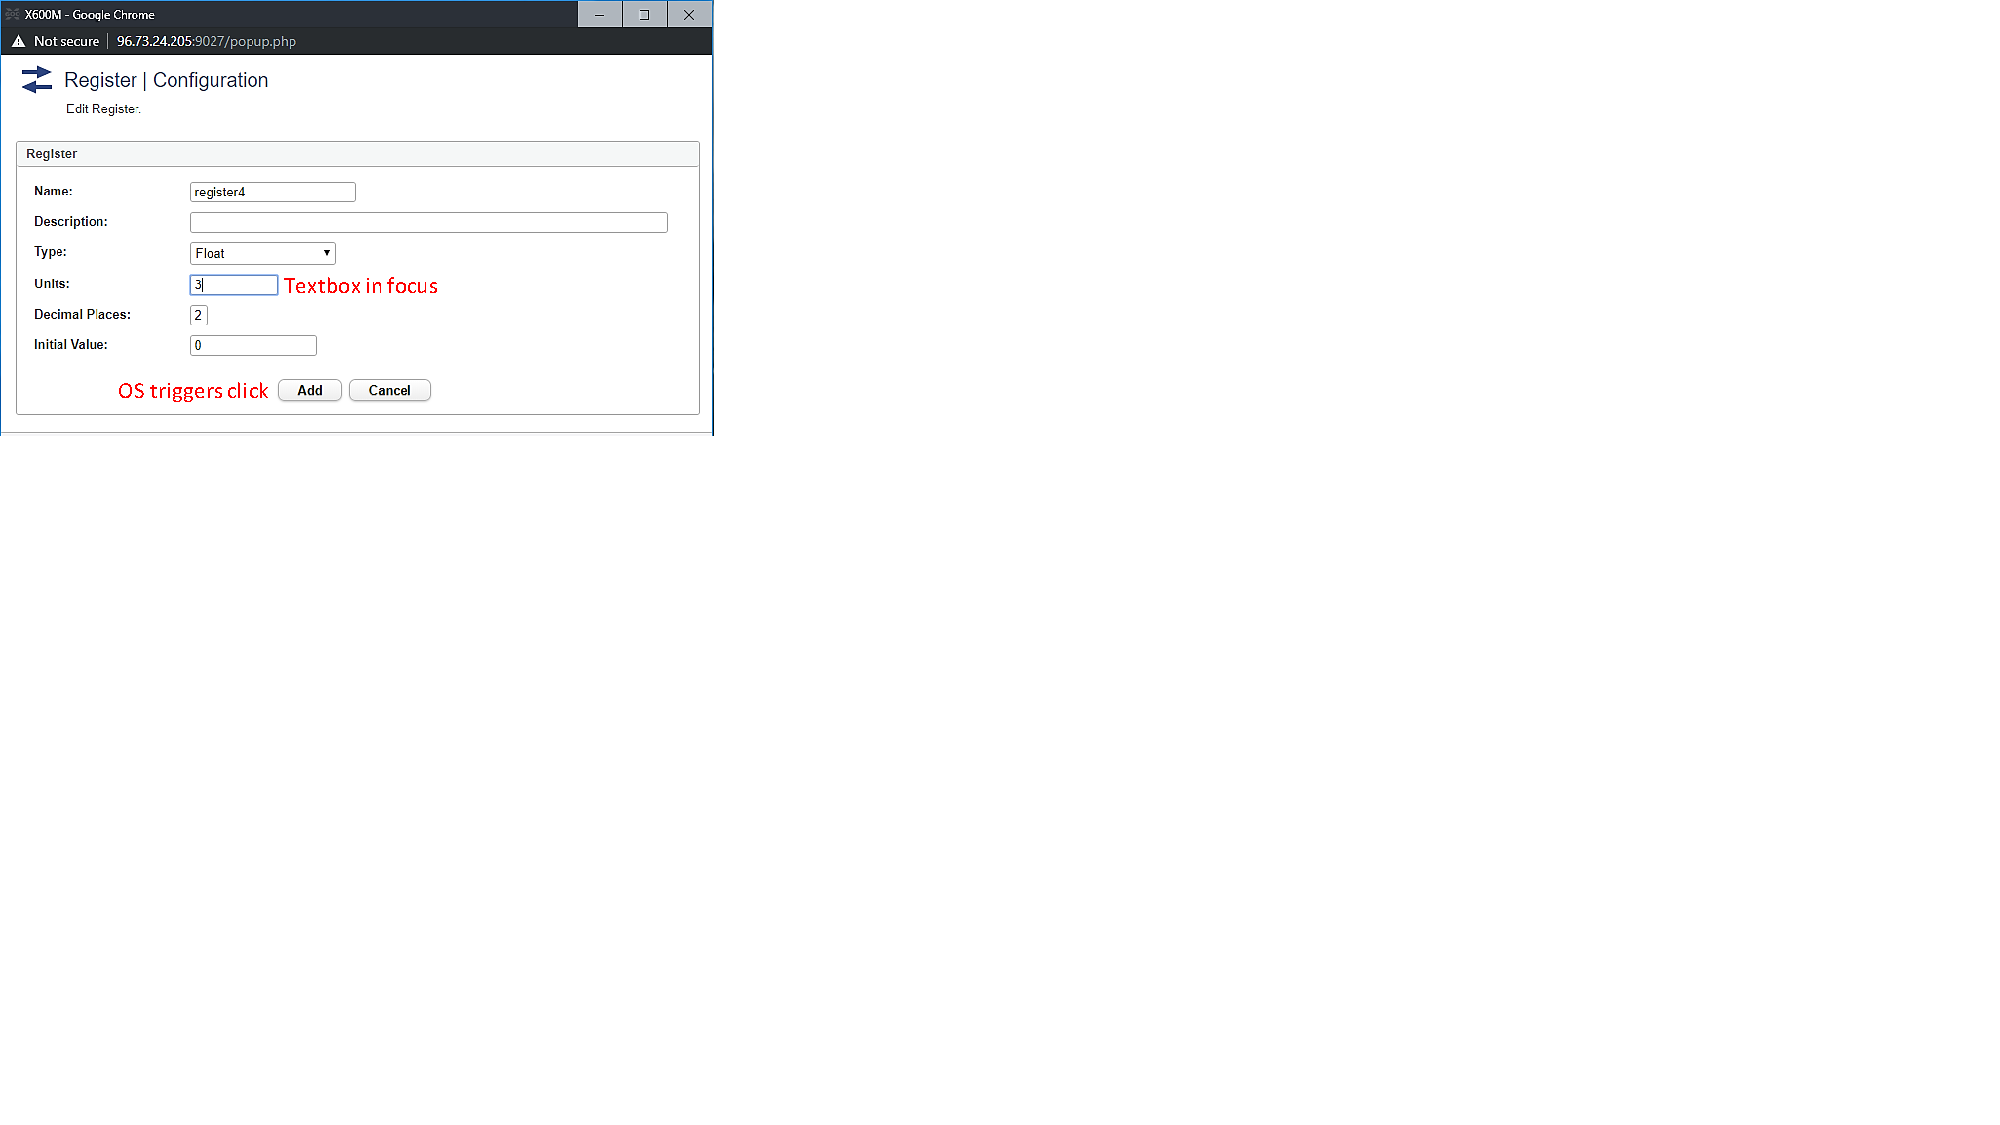
\includegraphics[trim={0 11.5cm 21.8cm 0}, clip, width=0.8\linewidth]{chapters/ProtectIOn/images/earlyFormSubmission.pdf}
\caption[Early form submission attacks]{\textbf{Early form submission attack} is possible on Fidelius~\cite{Fidelius}. The user selects and edits the field \emph{Units} while the OS triggers \emph{add} button, causing misconfiguration of a remote safety-critical PLC (Control by Web X-600M~\cite{controlbyweb}).}
\label{fig:clickJack}
\centering 
\end{figure}

Fidelius~\cite{Fidelius} addresses the problem with output integrity by rendering overlays using an external trusted device. Fidelius uses the trusted external device and Intel SGX to create a secure channel between the user IO devices and a remote server. The device intercepts user keystrokes and does not deliver any event to the untrusted host when the user types to secured text fields. Additionally, Fidelius renders an overlay with the user inputs on the screen, which is inaccessible by the host. This way, the untrusted host does not have access to raw inputs while the user sees them rendered on the screen as usual.
%provides secure input and display for the character-based device - keyboard. It uses overlays on the text fields to hide the keyboard input from the compromised host so that the input is only visible to the user. 
A small, trusted bar on display is also overlaid by the device that shows the remote server's identity and the text field that is currently selected. 
However, we observe a number of security and functional issues in Fidelius that we explain in the following. 

The overlay contains only the render of the user inputs into text fields, but the rest of the screen is rendered by the untrusted host.
This allows an attacker to modify the instructions on the UI, such as changing the input unit (typically described in the label of a text field) that could result in an incorrect input. This problem could be mitigated if the trusted bar includes the legitimate labels of the text fields also, although it would significantly increase the cognitive load to users.

%Fidelius solely relies on the static overlay bar and the LEDs on the external device to ensure the integrity and confidentiality of the input. 
Fidelius already introduces a high cognitive load to users as they need to monitor multiple security indicators simultaneously before filling up one text field. Previous research works~\cite{egelman2008you,sobey2008exploring, anderson2016warning} have shown that systems that require users to observe multiple security indicators %that require the users to observe multiple markers on the screen (and also on an external device) 
do not guarantee security in practice.
Also, in specific scenarios, even the training to properly explain these indicators to users could be a significant drawback for a real deployment.


\begin{mybox}[colback=white]{Observation 2}
If the \emph{protected output} is provided out-of-context, users are more likely not to verify it. Therefore input integrity can be violated.
\end{mybox}

%\noindent\emph{$\rightarrow$ Observation 2}: If the \emph{protected output} is provided out-of-context, users are more likely not to verify it. Therefore input integrity can be violated.


Fidelius does not consider the integrity of the mouse pointer and its interaction with UI elements, which broadens the attack surface. The lack of mouse support may appear to be a functional limitation, but it has non-trivial security issues.
The OS can arbitrarily trigger a mouse click on the submit button of a form while the user is typing and therefore send incomplete data to the server - early form submission attack.
This attack could cause the misconfiguration of a remote system, as illustrated in Figure~\ref{fig:clickJack}. Early form submission may appear to be similar to clickJacking attack, but the fundamental difference between them is that in clickjacking, the browser and OS are considered to be trusted. An untrusted OS can simply issue mouse clicks.

Moreover, Fidelius is also vulnerable to clickjacking attacks where the attacker can spawn a fake mouse pointer and trick the user into following it while the real mouse pointer is on a sensitive text field protected by the system. This allows the attacker to fool the user into providing (possibly incorrect) input while the user thinks that she is interacting with a non-sensitive text field. To prevent such attacks, the user has to look at the security indicators continuously even when she is not doing any security-sensitive task, which is a very strong assumption. 
Thus, not supporting the mouse causes the integrity violation of the keyboard input also.


\begin{mybox}[colback=white]{Observation 3}
If not \emph{all the modalities of inputs} are secured simultaneously, none of them can be fully secured.
\end{mybox}

%\noindent\emph{$\rightarrow$ Observation 3:} If not \emph{all the modalities of inputs} are secured simultaneously, none of them can be fully secured.


Finally, the design of Fidelius~\cite{Fidelius} is strictly limited to text-based fields only. As Fidelius does not provide output integrity of the forms, it cannot provide confidentiality to other UI elements such as radio buttons, drop-down menus, sliders, etc.
Microarchitectural attacks on Intel SGX~\cite{van2018foreshadow} increase the attack surface of the system significantly.


\myparagraph{B3. System TEE-based solutions} VButton~\cite{li2018vbutton} uses ARM TrustZone (TZ) to render UI buttons and receive user input from them securely. This is possible on mobile devices because the TZ architecture support flags on the system bus indicate whether an IO device like a touchscreen communicates with a trusted TZ application or the untrusted OS. Such solutions are infeasible for us because of the two following reasons. I) Secure communication between IO peripherals and TEE applications (like SGX enclaves) is not supported in the x86 architecture -- a similar system in x86 would require changes to the system architecture, TEE architecture, and IO devices. II) such solutions require TEE-aware applications and do not work with current browsers. Our goal is to design a solution that can be deployed on current x86 architecture and used with existing popular browsers.

\myparagraph{Strawman solution: Capturing screenshot} This strawman solution uses a trusted device that takes a screenshot when the user executes an action, e.g., mouse click to submit a form. The device then signs the snapshot and transmits it to the server along with the signed input. The remote server verifies the signature and then uses image/text analysis to extract the information from the UI elements such as labels on buttons or markers of a slider, etc. Therefore, the server would detect if the host has manipulated UI elements when presented to the user.

This method is vulnerable to attacks because it does not capture the spatio-temporal user context. This implies that the attacker may show some spatial information on the screen to influence the user that the snapshot may not capture. Furthermore, taking a full-screen snapshot could also reveal private information of the user from other applications. Similarly, taking a snapshot does not guarantee that a specific UI has been presented on the screen, as the attacker may render the legitimate UI shortly before the device captures the snapshot.
One way to mitigate this problem is to capture a video of user interaction. But such a method requires the host to send large amounts of data to the server, while the server should support video processing for different browsers, which is both time and CPU-intensive. Lastly, adversarial machine learning techniques~\cite{eykholt2017robust,sitawarin2018rogue} make the image/text recognition techniques insecure against advanced adversaries.


\subsection{Requirements of Security and Functional Properties}
\label{sec:problemStatement:goals}

We can summarize the above-discussed limitations of previous solutions as the following requirements for our solution:

\myparagraph{R1. Inter-dependency between input and output} 
The first and second observations from the existing solutions show that the output and input security depend on each other, and they should be considered together. Otherwise, the attacker can manipulate the output to influence the user input.

\myparagraph{R2. Inter-dependency between all input modalities} 
Existing web interfaces allow users to complete forms using different modalities for user input, namely the keyboard, the mouse, and the touchpad. The third observation shows that a secure system should simultaneously protect all user input modalities to achieve input integrity (against early-form submission and clickjacking).


\myparagraph{R3a. No cognitive load for IO integrity} 
A system that protects IO operations should introduce minimal or no cognitive load to its users for input integrity.
The system should guarantee the output integrity of the legitimate information necessary to complete a form and avoid asking the user to interact with an external device or monitor security indicators out-of-context.


\myparagraph{R3b. User attention for IO confidentiality} Preserving the confidentiality of user inputs against a compromised host is a challenging task because the host can trick the user into revealing her inputs when the system is not active. Therefore, requiring users to perform a small action, e.g., press a key before entering confidential inputs, is a valid tradeoff between usability and security.


\myparagraph{R4. Small trust assumptions and deployability} 
Our goal is to provide a rich set of IO and security features with minimal trust assumptions that do not rely on a trusted OS, specialized hypervisor, or TEEs such as Intel SGX. Preferably, the solution should be easy to set up for users, i.e., plug-and-play, and integrate well with the existing infrastructure.  

\section{System Overview \& Main Techniques}
\label{sec:approach_protection}

\begin{figure}[t]
\centering
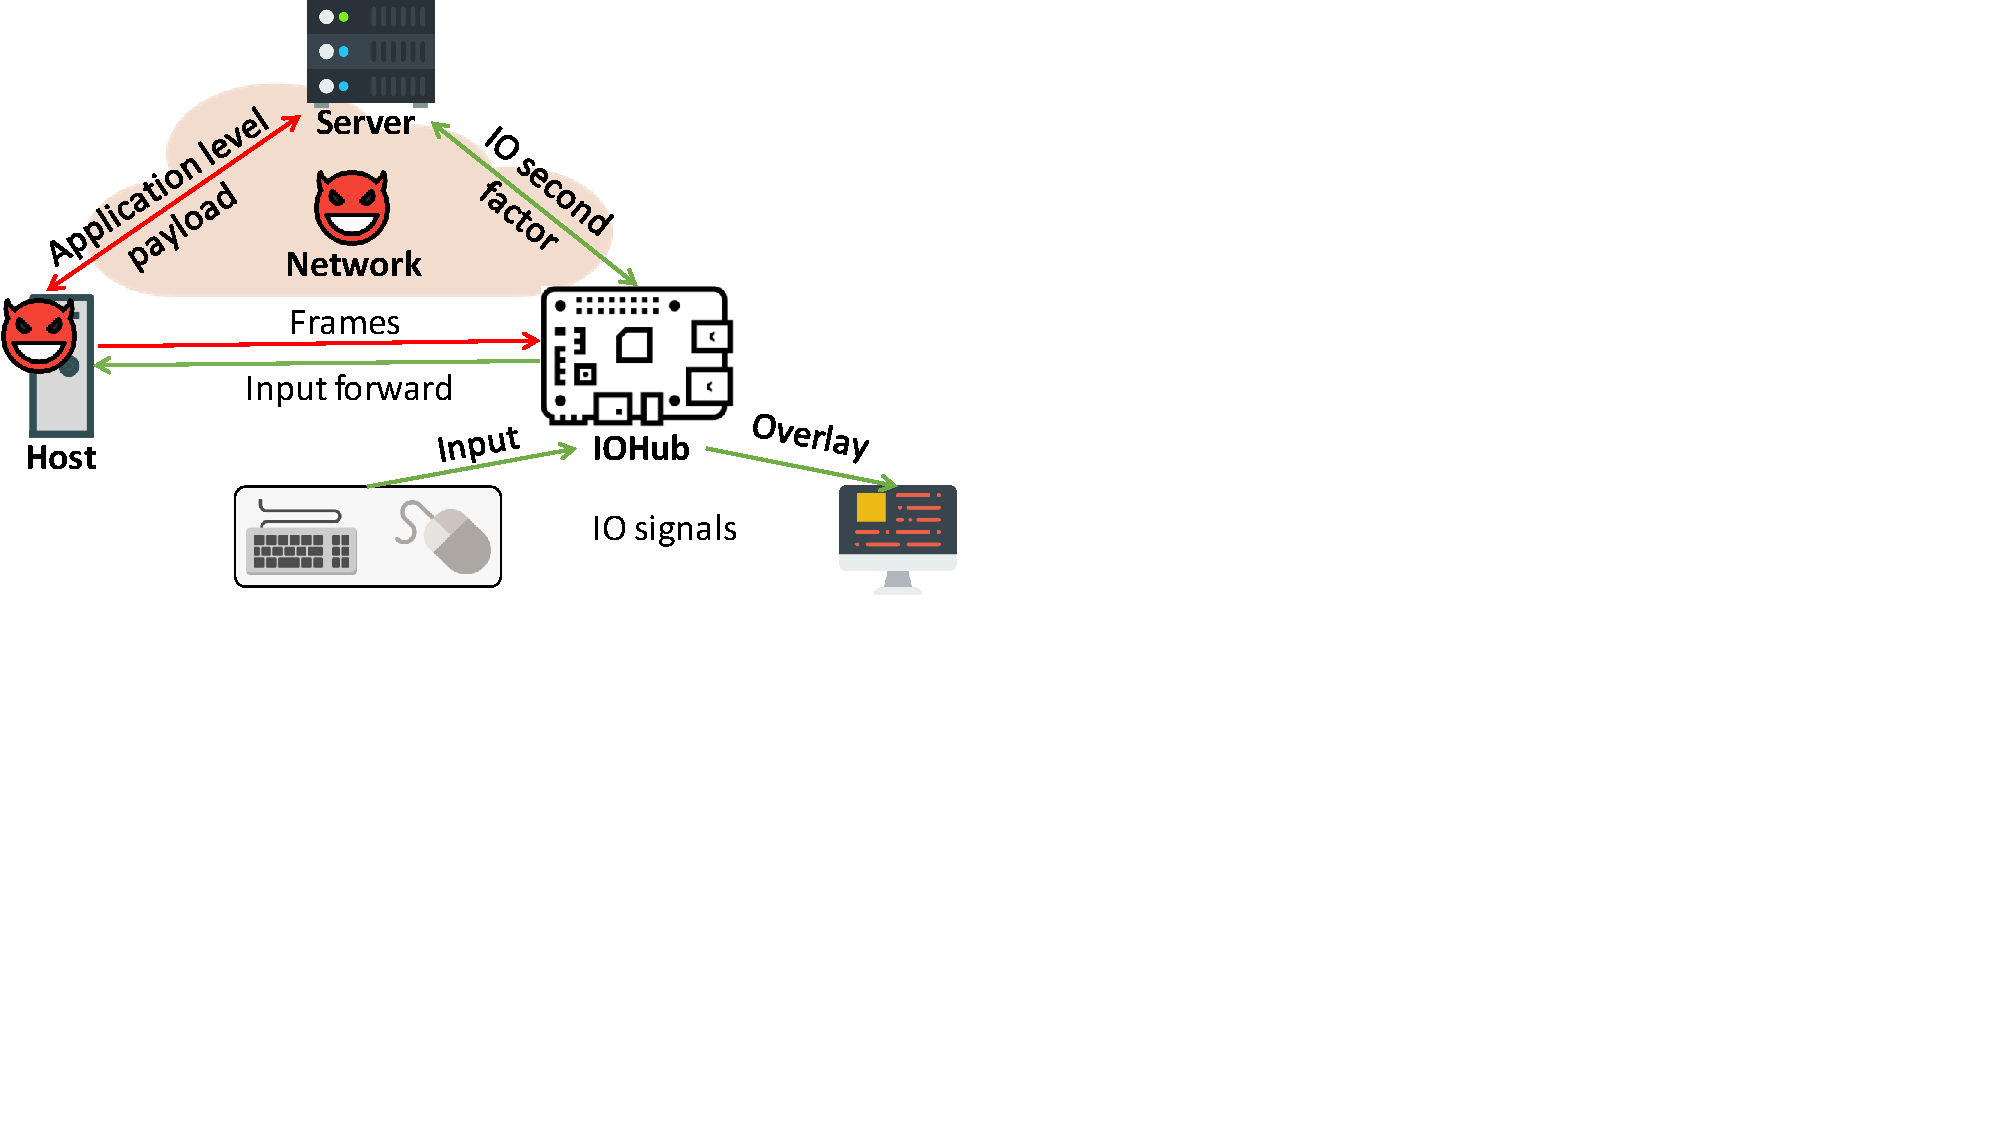
\includegraphics[trim={0 8.5cm 17cm 0}, clip, width=0.8\linewidth]{chapters/ProtectIOn/images/approachOverview.pdf}
\caption[High-level approach overview of \name]{\textbf{High-level approach overview of our solution.}  The \device connects the trusted IO devices and the attacker-controlled host.}
\label{fig:approachOverview}
\centering
\end{figure}



In this section, we present an overview of our solution: \name. On the high-level, \name uses the concept of the \emph{bump in the wire} (such as bump in the ether~\cite{McCPerRei2006}) to provide integrity and confidentiality to the user IO{}s between the IO devices and the remote server. \name achieves this by utilizing a trusted embedded device as a mediator between all the IO devices and the untrusted host. Hence, our approach falls into the category \textbf{B2} (external HW) in Figure~\ref{fig:relatedWorksTree}. We call this trusted intermediary \device. 


\subsection{System and Attacker Model}
\label{sec:approach:systemAttackerModel}

We consider a typical scenario where the user wants to interact with a trusted remote web server via an attacker-controlled host. The model is depicted in Figure~\ref{fig:approachOverview}, which shows the untrusted host, the remote server, and the user IO devices. We only assume that the monitor, keyboard, mouse (in a word all the IO devices that we need to protect from the malicious host), and the \device are trusted. One benefit of an external trusted device is that regulations may prevent modifications of systems such as medical devices. However, retrofitting them with external devices, such as the IOHub, is usually possible.

The \device works as a mediator between all the IO devices and the host. Note that the \device has no network capability to communicate with the server directly, instead it relies on the host and uses it as an untrusted transport. We also assume that the \device comes with preloaded certificates and keys that allow the \device to verify the signatures signed by the server and sign data such as the user input.

\myparagraph{Deployment options}
There are several possible ways to deploy the \name system. Here we outline two example cases. The first example deployment is one where a service provider, like a bank issues a \device device to each of its customers. In such a deployment, the issued \device is intended to be used with a single application like a web-based online banking application, and it is pre-configured with the public key certificate of that application server (e.g., online banking server). The pre-installed certificate allows the \device to verify messages signed by the correct application server. The service provider (i.e., the issuer of the \device) can ask what OS the customer uses and configure OS-specific settings like the used SAS value to the issued device (see Section~\ref{sec:confidentiality:SAS} for details). 

In another example deployment, the \device is issued by a third-party vendor, and it is intended to be used to protect the user interaction of various security-critical online services. In such a deployment, the \device can be pre-configured with the public key of its issuer and a white-list of trusted application server certificates. The issuer of the device can issue authenticated updates to the white-list after its deployment if needed.

\myparagraph{Attacker model and capabilities} Our attacker model assumes that the host (OS, installed applications, and hardware) and the network are attacker-controlled. The attacker can intercept, and arbitrarily manipulate (such as create, drop, or modify) the user IO data between the user and the remote server. Furthermore, we assume that the attacker can not break the physical security of the \device (more discussion in Section~\ref{sec:securityAnalysis:device}).
 


\subsection{High-level Description of the System}

\begin{figure}[t]
\centering
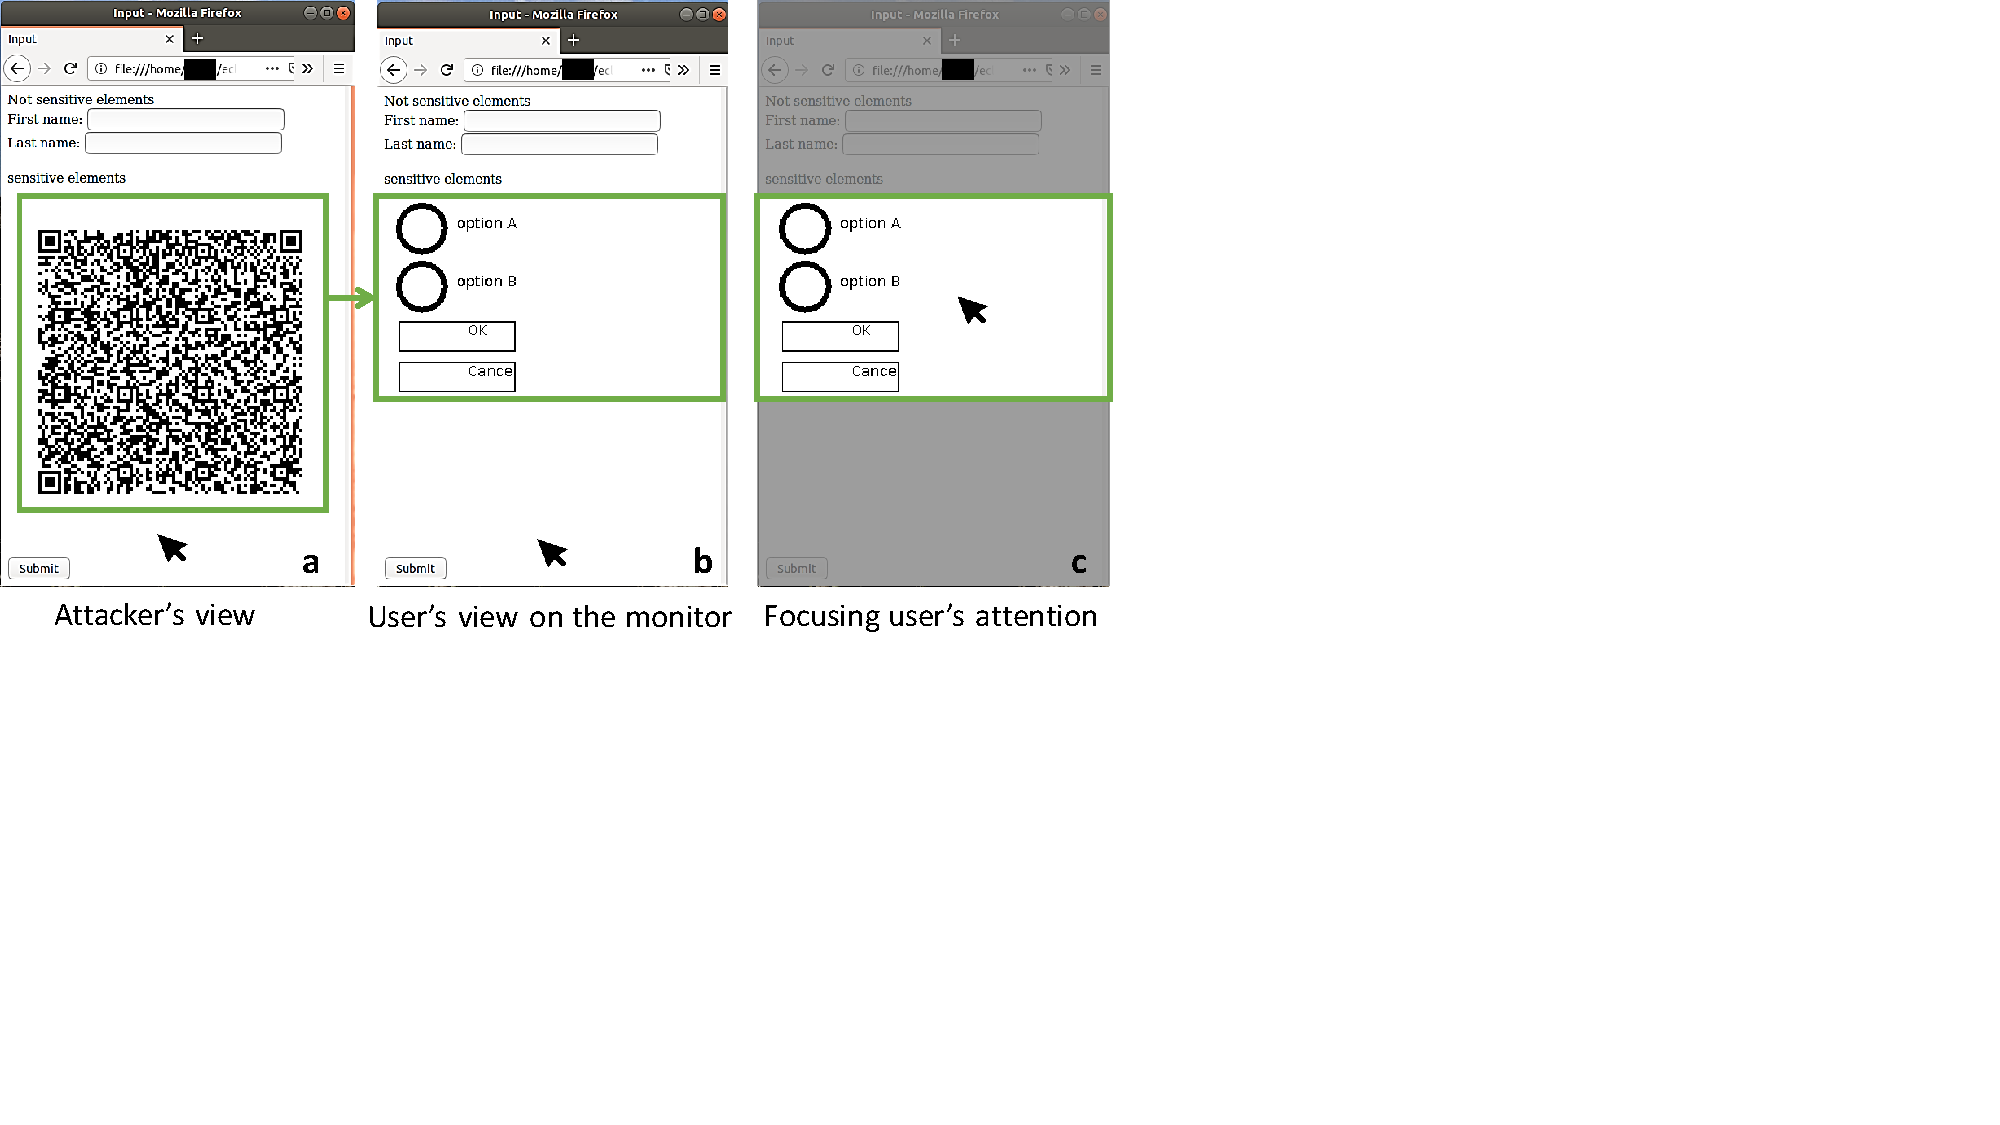
\includegraphics[trim={0 8cm 15cm 0}, clip, width=\linewidth]{chapters/ProtectIOn/images/overlayScreenShot_new.pdf}
\caption[\name's high-level approach for UI overlays]{\textbf{\name's high-level approach for UI overlays} shows that the \device generates UI overlay to protect IO integrity and confidentiality. a) The attacker only sees the non-protected UI elements, and the protected form is encrypted and encoded (in our case, the \device could decode a QR code and decrypt). b) shows the \device generated form overlay that is hidden from the host. The protected part of the screen provides integrity and confidentiality of all user IO. c) shows that the \device dims out (lightbox) the rest of the screen when the user moves her mouse pointer over the protected region to focus user attention.}

\label{fig:screenshot_1}
\end{figure}

\name is built upon the security requirements and functional properties that are described in Section~\ref{sec:problemStatement:goals}.
\device is active only when the user visits sensitive web applications that require \name security.
Initially, the remote server signs and delivers the sensitive UI elements to the host in a format that is understandable by \device. Next, the host transfers the sensitive UI to \device, and the \device verifies the signature to prevent manipulations by the host. As seen in a running example depicted in Figure~\ref{fig:screenshot_1}, the \device then renders the UI with sensitive elements into an overlay on top of the HDMI frame received from the host. Note that the host cannot access or modify the overlay generated by the \device. Also, the overlay covers only a part of the screen, allowing the other feature-rich content on the webpage to run unmodified. Therefore, this ensures that sensitive UI elements are presented to the user as expected by the remote server -- \emph{output integrity}. For the overlay, we use QR-codes to transfer data from the host to the device because we avoid using extra software/hardware for a separate channel, and it is easy to visualize.

When the user interacts (types or moves the pointer) with the overlay, \device does not forward any event from the keyboard or the mouse to the host. The interaction is maintained solely by \device, which renders on-screen user inputs and therefore offers a user experience that is identical to a typical one as if the \device is not present. The user clicks on the \emph{submit} button triggers the submission procedure, which consists of the \device signing the user inputs and sending it to the server. Note that the text fields of the form and the \emph{submit} button are inside the overlay, which is inaccessible by the host, hence the attacker cannot execute the early form submission or clickjacking attacks. Finally, the server verifies the signature of \device to guarantee that the host has not altered the data. Therefore, the \device ensures \emph{input integrity} for all \emph{modalities} of input.

For integrity guarantees, \name uses well-known user attention focusing mechanisms. Unlike systems like Fidelius, these mechanisms do not introduce any cognitive load to the users as \name does not rely on multiple security indicators. Mechanisms such as lightbox aid the user to distinguish the \device overlay on the screen from the rest. Thus, the untrusted host cannot trick the user into following malicious instructions when the user interacts with sensitive UI elements. In the case where confidentiality is required, the user manually triggers SAS, using a well-known sequences of keys such as \emph{Ctrl+Alt+Del} that highlights the sensitive UIs using mechanisms such as lightbox (see Section~\ref{sec:confidentiality:SAS} for details). For confidentiality, the host cannot observe the overlay and user input as they are encrypted by the TLS key between the \device and the server.


\begin{figure*}[t]
\centering
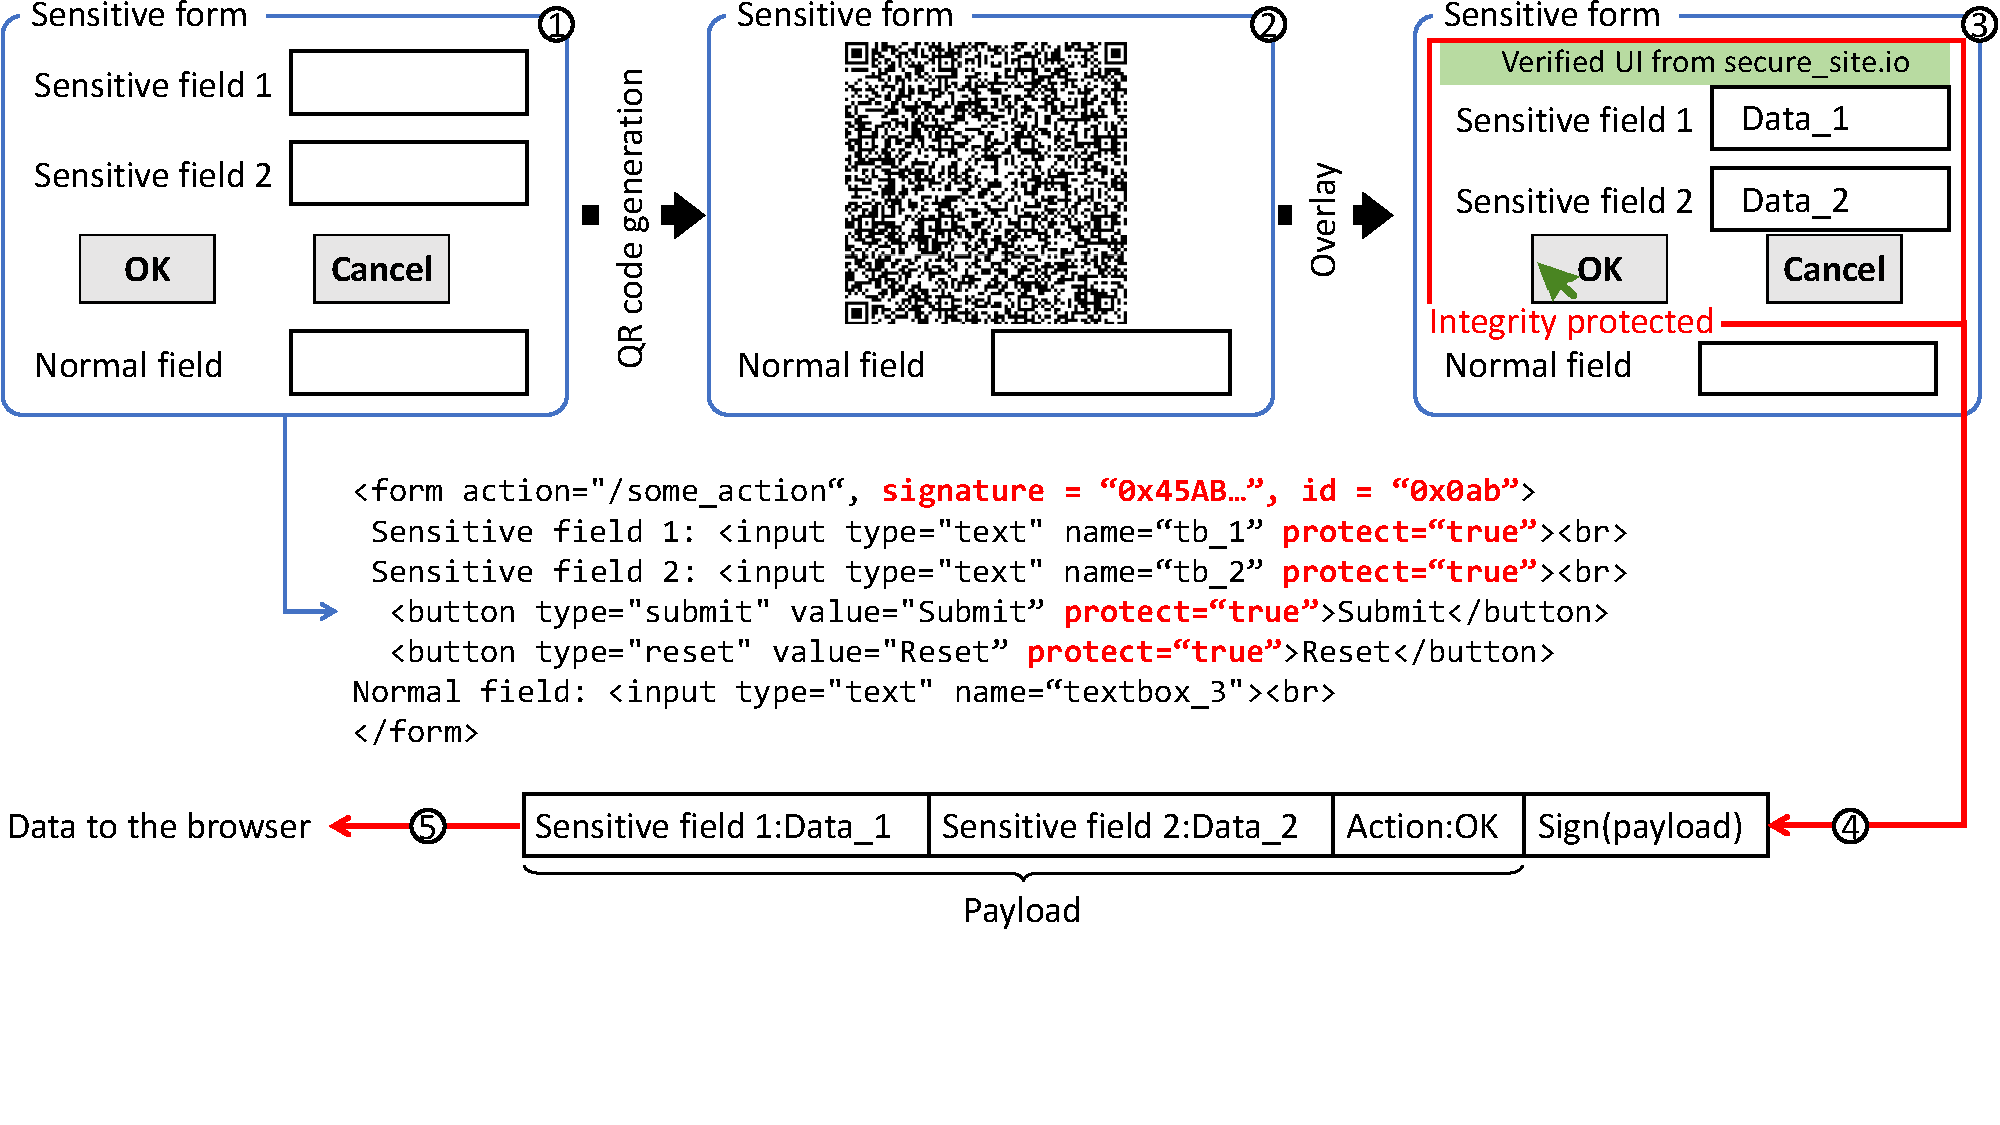
\includegraphics[trim={0 4cm 0 0}, clip, width=\linewidth]{chapters/ProtectIOn/images/formTransform.pdf}
\caption[Transformation of UI elements: HTML $\rightarrow$ encoded specification $\rightarrow$ \device generated UI overlay]{\textbf{Transformation of UI elements: HTML $\rightarrow$ encoded specification $\rightarrow$ \device generated UI overlay.} \one The actual webpage and the corresponding \html source shows the UI elements that requires integrity protection. \two These UI elements are transformed into an encoded UI specification (our \name prototype uses QR code that encodes a UI specification, e.g., Specification~\ref{snippet:UISpecification}) by the \name JS. The QR code. \three AThe QR code decoded and overlaid on the HDMI stream by the \device. \four Upon the user's action on the overlaid UI elements, the device signs all the input data. \five The \device sends these signed input data them to the remote server. Note that the intermediate QR code transformation (\two) is not visible by the user.}
\spacesave
\label{fig:transformation}
\end{figure*}

\section{\name for IO Integrity}
\label{sec:protection}



\lstset{language=JSON, frame=tb, caption=\textbf{Protected UI specification language.} The UI specification shows the JSON formatted UI specification that is generated from the \html source provided in the UI illustrated in Figure~\ref{fig:transformation}., label=snippet:UISpecification, firstnumber =1}

\begin{figure}[t]
\scriptsize
\begin{lstlisting}[mathescape=true]
{ "formId": "form1", "formName": "form1",
  "domain": "secure_site.io",
  "size": "400*400", "SAS": "5:LB",
  "ui": [{"id":"textbox_1", "type":"textbox", 
      "label":"Sensitive field 1",
    "text":"secret data 1",
    "RE":(A-Z)*.(A-Z)*},
    {"id":"textbox_2", "type":"textbox",
    "label":"Sensitive field2 ",
    "text":"secret data 2"},
    {"id":"b1", "type":"button",
    "label":"OK", "trigger":"true"},    
    {"id":"b2", "type":"button",
    "label":"Cancel", "trigger":"false"}],
  "signature": "0x45AB...", "id": "0x0ab.."}
\end{lstlisting}

\end{figure}

%In this section, we provide the technical details of \name for the integrity protection of IO devices. 
In this section, we provide the technical details of \name that guarantees the integrity of IO operations.


\subsection{\device Overlay of UI Elements}
\label{sec:systemDesign:transformation}

As we explained in the previous sections, both output and input integrity are necessary to be protected to achieve any of them. \name ensures output integrity by isolating a part of the display that cannot be observed or modified by the untrusted host. \device intercepts the HDMI frame from the host and injects a render of the sensitive UI on the screen. The overlay provides output integrity because it restrains the attacker from drawing on top of it to trick the user into providing incorrect inputs. 

Our goal is to minimize the TCB, and thus the \device does not run a browser, i.e., it cannot interpret or render HTML, \js, etc. Given this constraint, one strawman solution could be sending UI bitmaps from the server to the \device, and the \device could send back the mouse click and the corresponding location. \device could download these pre-generated form bitmaps from the server, and such a solution would handle static forms, but not for dynamic forms. Downloading all possible form bitmaps would be prohibitively expensive.

To achieve a more generic and efficient solution, we follow a different approach. The \device comes with a small interpreter routine that is similar to render engines of browsers in functionality, but drastically smaller in size because it only renders a limited number of HTML5 UI elements according to their position, dimension, and label. The interpreter routine reads a given specification and renders the respective UI. The specification is a simple \emph{JSON} file that defines how the content of the overlay should be rendered, e.g., number of elements, order, types, and labels.  

The process of rendering the overlay on the screen has two phases: (i) convert the existing sensitive form to specification, and (ii) specification to overlay.

\myparagraph{(i) Secure form $\rightarrow$ Specification} The W3C UI security policy~\cite{w3c_spec} recommends developers to annotate the security-critical UI elements of a page to protect them against malicious JS running on the browser. We use a similar technique by asking developers to manually annotate the sensitive elements in the HTML code (as \emph{protect=``true''} attribute). Then For every request, the \name server-side component parses the HTML source, adds a random identifier (\texttt{id}) to the \texttt{form} element, signs it, add the \texttt{signature} to the \texttt{form} and then delivers it to the user's browser. The \texttt{id} serves as session identification to prevent the attacker from re-submitting an old input data from the user. On the host-side, \name JS parses the tagged HTML source and produces a specification that can be interpreted by the \device.  An example of a specification is presented in~Specification~\ref{snippet:UISpecification}. In our implementation, the \name JS encodes the specification in a QR code. \red{(\#5)We choose QR codes to encode UIs as it is one of many robust ways to encode data on a visual channel such as HDMI stream.} Figure~\ref{fig:transformation} shows the transformation between the step \one and \two. The step \two is processed by \device in the next phase and is not visible to the user.


%We further optimize this process that does not require to add the UI specifications into the HTML sources. The developers include small JavaScript code: \name JS to their sources. \name JS has the same functionally as the server-side code that parses the HTML code and outputs the specification. Note the specification generation process is deterministic, hence, given identical HTML sources, both server and the \name \js generate identical UI specifications. Note that \name JS runs on the browser and is not trusted in our system model. We illustrate the method of UI transformation in Figure~\ref{fig:transformation}. 


\myparagraph{(ii) Specification $\rightarrow$ Overlay} \device performs the next phase, which starts with the detection of the encoded specification (QR-code) in the HDMI frames. Then the \device validates the signature, renders the overlay according to the specifications, and presents it to the user.  The \device overlay is depicted in \three in Figure~\ref{fig:transformation}, which is the final UI shown to the user. Note that the user does not see the QR code as it gets decoded and overlaid by the \device on the fly.

\device uses the specification to determine the particular UI element that the user interacts with. When the user clicks on a text field, \device allows the user to type input to it. UI elements in the overlay take inputs only from input devices (mouse and keyboard). Therefore a malicious host cannot inject or modify any input of the user.

\subsection{Focusing User Attention}
\label{sec:systemDesign:userAttention}

In the previous section, we explain how \name provides output integrity for the overlay generated by the \device. However, the attacker can show fake information to the user on the untrusted part of the display space that may potentially influence her inputs. An advanced adversary could craft malicious directions and present to the user as part of the overlay.

To mitigate these attacks, we employ techniques that are proposed against similar threats in the context of browser-based security. The goal of these techniques is to focus user attention on the sensitive UI elements she is interacting with. Huang et al.~\cite{huang2012clickjacking} proposes two main techniques that are shown to be effective and can easily be adopted by the \device.  The first technique is called Lightbox, and it dims out the non-overlaid part of the screen, which is generated by the untrusted host. The second technique consists of freezing display frames from the host when the user enters into the overlaid UI. This way, a malicious host cannot grab the user's attention by showing an animation or exploiting other tricks.
Lightbox offers more security guarantees because it blocks the untrusted screen completely, but is more intrusive to the user. While freezing is less intrusive but does not remove potential malicious information from the screen.

Lightbox mitigates the attacks presented above. The paper shows that the Lightbox and freezing are effective in $98\%$ and $97\%$ of the time (baseline: $69\%$ effectiveness when no protection is provided), respectively, making them suitable candidates for \name. For more details of the user study, refer to Table 2 in~\cite{huang2012clickjacking}. We assume that a similar result should be expected in \name due to the similarity of the application space (web applications). \device uses Lightbox as the default technique, but depending on the specific form, the developers can select the appropriate technique.

When the focusing mechanism (e.g., LightBox) is active, the user can still interact with the UI elements and browser button outside the secure UI elements as the \device does not control those. Browser back button does not influence the state of the overlaid UI as long as it does not remove/change the QR code on the web page.


\myparagraph{\bfseries Automated activation} The technique to focus user attention (dimming out or freezing the non-overlaid part of the screen) is triggered automatically in specific situations: The user moves the mouse pointer over the overlaid UI, or the user starts typing into a sensitive UI element. 
%e.g., when the user moves her mouse pointer over the overlaid UI, or start moving the mouse after a brief pause (like 5 seconds). 
The advantage of the automated trigger is that the user does not need to remember to activate the mechanism. Hence the system is resilient from user habituation and does not require the user to monitor security indicators actively or perform specific actions. Note that the automated activation provides security to user IO data \emph{only} when the integrity of the data is considered.

\subsection{Continuous Tracking of Mouse Pointer in the HDMI Frame}
\label{sec:systemDesign:analysis}


\begin{figure}[t]
\centering
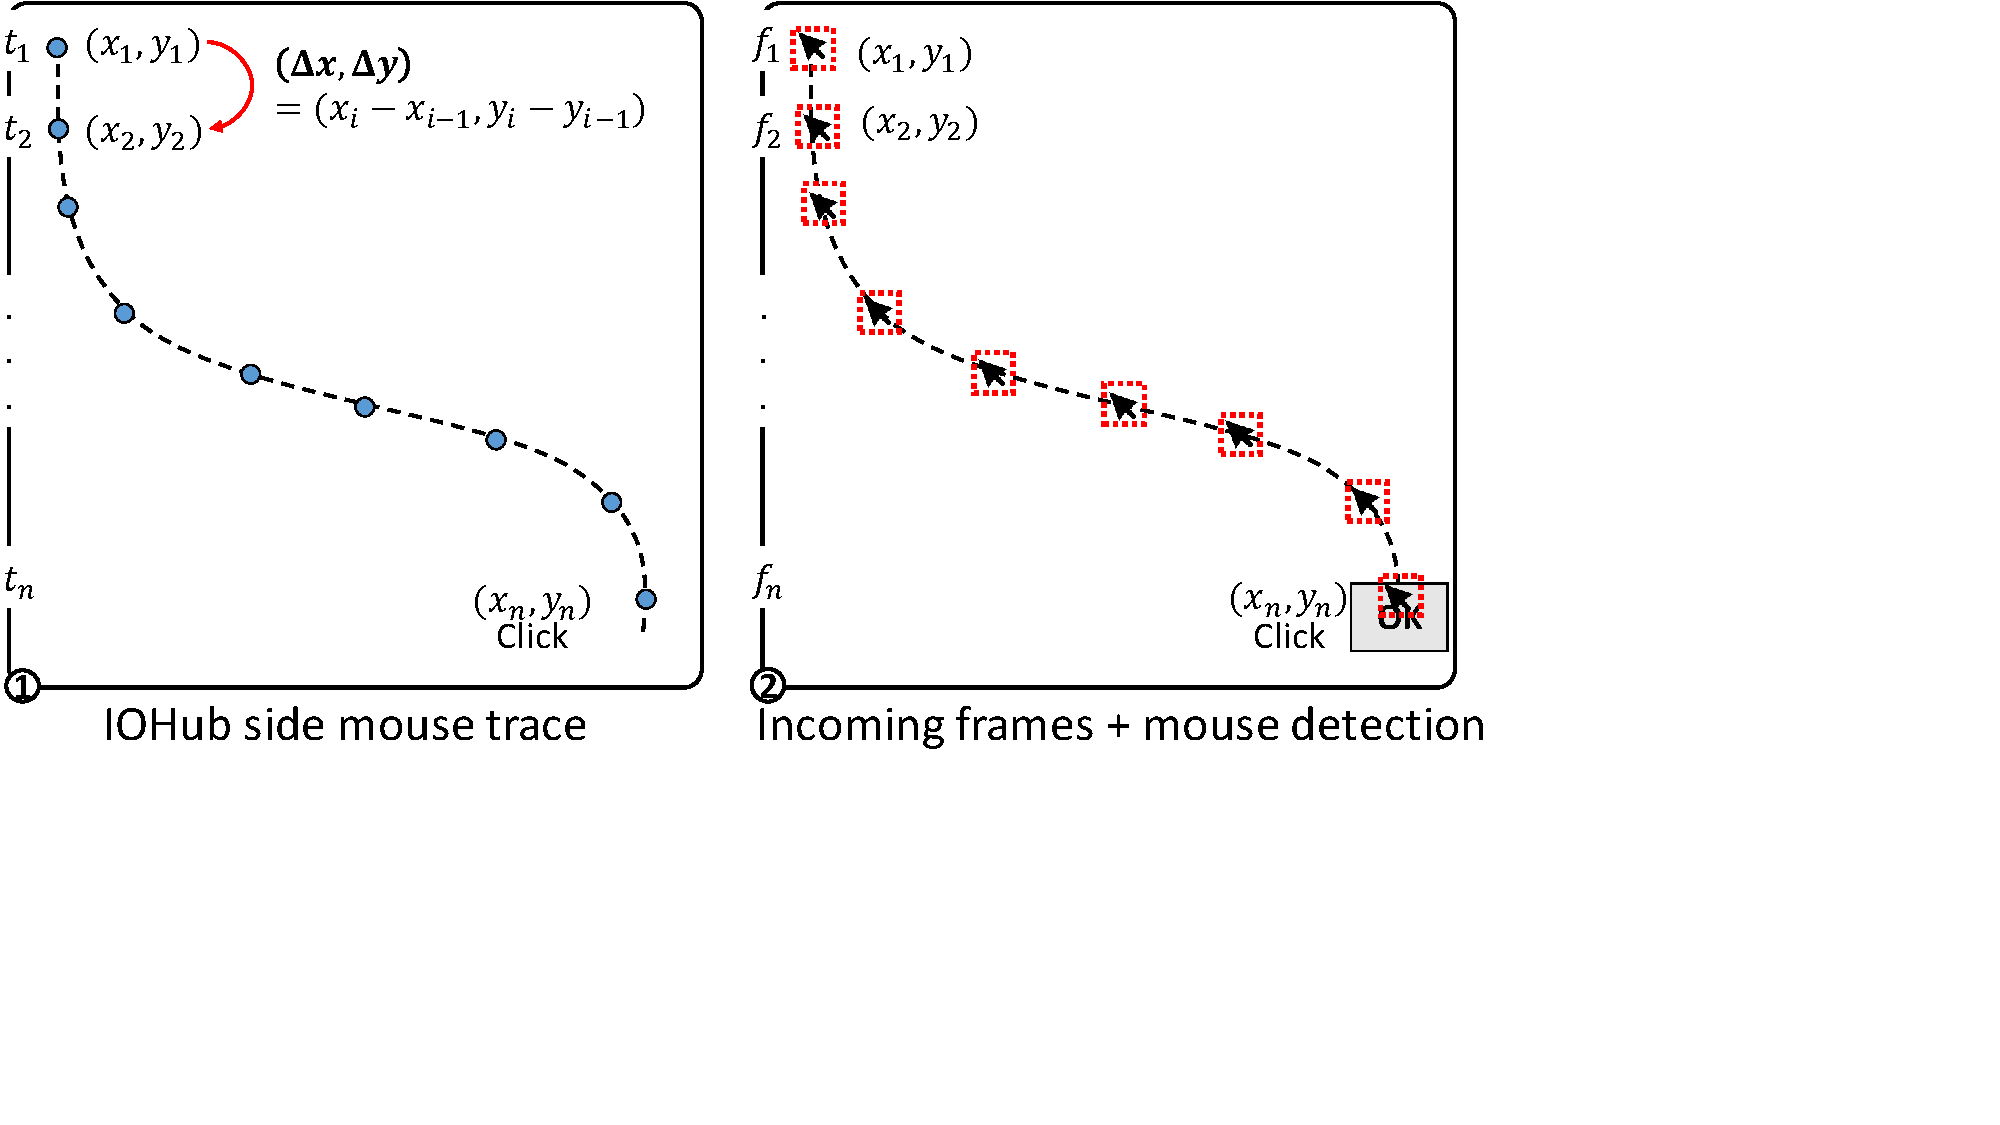
\includegraphics[trim={0 5.2cm 8cm 0}, clip, width=0.9\linewidth]{chapters/ProtectIOn/images/mouseAnalysis.pdf}
\caption[\name Pointer tracking]{\textbf{Pointer tracking.} \one The \device captures the raw mouse events ($\Delta x, \Delta y$) from the mouse that is attached to the \device. \two The \device captures the frames from the HDMI channel and checks into the designated pixel position $(x_i + \Delta x, y_i + \Delta y)$ if there exists a pointer. $t_1, t_2,\ldots t_n$ are the time instances when the \device receives the mouse data. $f_1, f_2,\ldots f_n$ are the corresponding HDMI frames that the \device intercepts.}
\spacesave
\label{fig:mouseAnalysis}
\centering
\end{figure}


The triggering of the focusing mechanism poses a challenging task to \name because the \device does not know the exact position of the mouse pointer. We cannot rely on the compromised host to communicate the pointer position reliably to \device. Furthermore, the host's pointer is not visible when the user interacts with the overlay rendered by the \device as the \device always draws on top of the HDMI frames of the host. 
%To address this issue, \name continuously tracks the host's mouse pointer from the HDMI frame (using shape detection) as it has access to both the HDMI channel and the raw mouse data.

\device could employ image analysis over the frame received from the host to learn the pointer position. However, we avoid this method because image analysis is time-consuming and vulnerable to adversarial images. In our approach, the \device intercepts mouse events and HDMI frames, so it can track the pointer based on mouse data and correlate it with the actual position in the HDMI frame (using shape detection in a small area). Then, the \device overlays a mouse pointer that is prominent and easy to follow by the user. 

A malicious host can still show a fake pointer to trick the user into following it, but when the focusing mechanism is active (the user interacting with sensitive elements), only the pointer overlaid by \device is visible. This way, the pointer tracking and the pointer overlay address three major challenges: i) both the \device and the user have the same sense of the pointer position, ii) \device precisely knows when to trigger the focusing mechanism, and iii) the user can interact with the overlaid UI seamlessly. 


\subsubsection{\bfseries Calibration}\label{sec:systemDesign:analysis:calibration} When the user connects the \device for the first time after booting up, the \device performs an automated calibration to find the pointer. The \device simulates the mouse and pushes the pointer to the top-right corner of the screen. Then the \device searches the pointer at this position in the HDMI frames
%If the \device is successful in finding the mouse pointer, 
and starts tracking the pointer afterward. Note, that at any point, if the \device loses track of the mouse pointer, the \emph{calibration} process is repeated the first moment the user visits a website that employs \name.
%user can recalibrate it by reinitializing the \device.

\subsubsection{\bfseries Pointer detection} The \device ensures pointer integrity by tracking the mouse movements using the raw data from the mouse and the HDMI frame.  Figure~\ref{fig:mouseAnalysis} illustrates the main idea: 

\begin{enumerate}
\item[]\one Shows raw mouse data that notify the displacement events $(\Delta x, \Delta y)$ over $x$ and $y$ axis which are fired over time series $t_1,\ldots, t_n$. Note that the initial pointer position is known to the \device from calibration phase where $(x_0, y_0) = (0, 0)$.  
\item[]\two Shows the HDMI frames $f_1,\ldots f_n$ where the \device expects the mouse pointer to be found. For efficiency, the \device only scans a small portion of the HDMI frames ($200 \times 200$ square pixels) that is enough to cover a mouse pointer. Since the operating system can treat mouse movements slightly different according to their algorithm, this step serves to adjust the position difference.
%\device checks if there exists a mouse inside this square or not. \red{In case there exists a mouse cursor, the \device allows further user interactions; otherwise, it stops all the communications and shows an error on display.}
\end{enumerate}


\subsubsection{\bfseries Overlay of the mouse pointer} The \device draws a mouse pointer overlay on top of the actual mouse pointer. The host mouse pointer is neither visible on top of the overlay nor it can interact with the \device's overlay. The overlaid mouse pointer is visible on top of the overlay, and it offers the same user experience as the host-rendered mouse pointer.


\subsubsection{\bfseries Coping with the disappearing pointer} Many OS offer a feature where the mouse pointer disappears from the screen when the user types in a text editor/browser. When the user moves her mouse, the cursor appears again in the same position where it disappeared in the first place. From the \device's perspective, it is hard to distinguish between this case and the attacker deliberately removing the mouse pointer from the screen. To handle this case, the \device listens to all the keyboard inputs -- the keyboard is also connected to the \device. Therefore, when the \device gets a keystroke event, it expects the cursor to disappear from the screen. Then, \device continues tracking the pointer from the moment that the mouse sends events  - this way, the \device ensures the consistency of the pointer position.  


\subsubsection{\bfseries Handling different mouse cursors} The \device is preloaded with template images of the mouse pointer for detection. For our \name prototype implementation, we use the default cursors provided by the Ubuntu OS. This allows the \device to identify the cursor when it changes on the screen, e.g., from pointer to a hand when the user hovers the pointer over a link on the browser. 

 
\subsubsection{\bfseries Handling mouse acceleration} The \device uses the default mouse acceleration parameters of \emph{libinput} to cope with the pointer acceleration. As the \device emulates itself as a keyboard, at the time of initialization, the \device sends a command to the host to set the default acceleration. In case the host changes the mouse acceleration, the \device will fail to detect the mouse in the HDMI stream. We consider this case as a denial of service.

\subsubsection{\bfseries Entering/exiting secure mode with keyboard} In our implementation of \name, entering and exiting the secure mode is performed by moving the mouse pointer into or out of the protected UI area (sensitive web form). 
%But similar could be done with the keyboard also.
This could similarly be done with the keyboard.
The user could use the \emph{TAB} button that selects the QR code (that is an image on the webpage) on the browser. When the QR code is selected, \name JavaScript triggers a change in the JSON specification that is encoded in the QR code. E.g., the specification contains a parameter named \emph{selected} that defines if the user is inside the secure mode or not. By changing this parameter, the \name JavaScript signals the \device that the user is currently in the secure mode. While inside the secure mode, the \device handles the \emph{TAB} signal from the keyboard, allowing the user to switch UI elements within the secure UI. When the user reaches at the end of the secure UI, the device returns control back to the \name JavaScript when the user presses \emph{TAB}.


\begin{figure}[t]
\centering
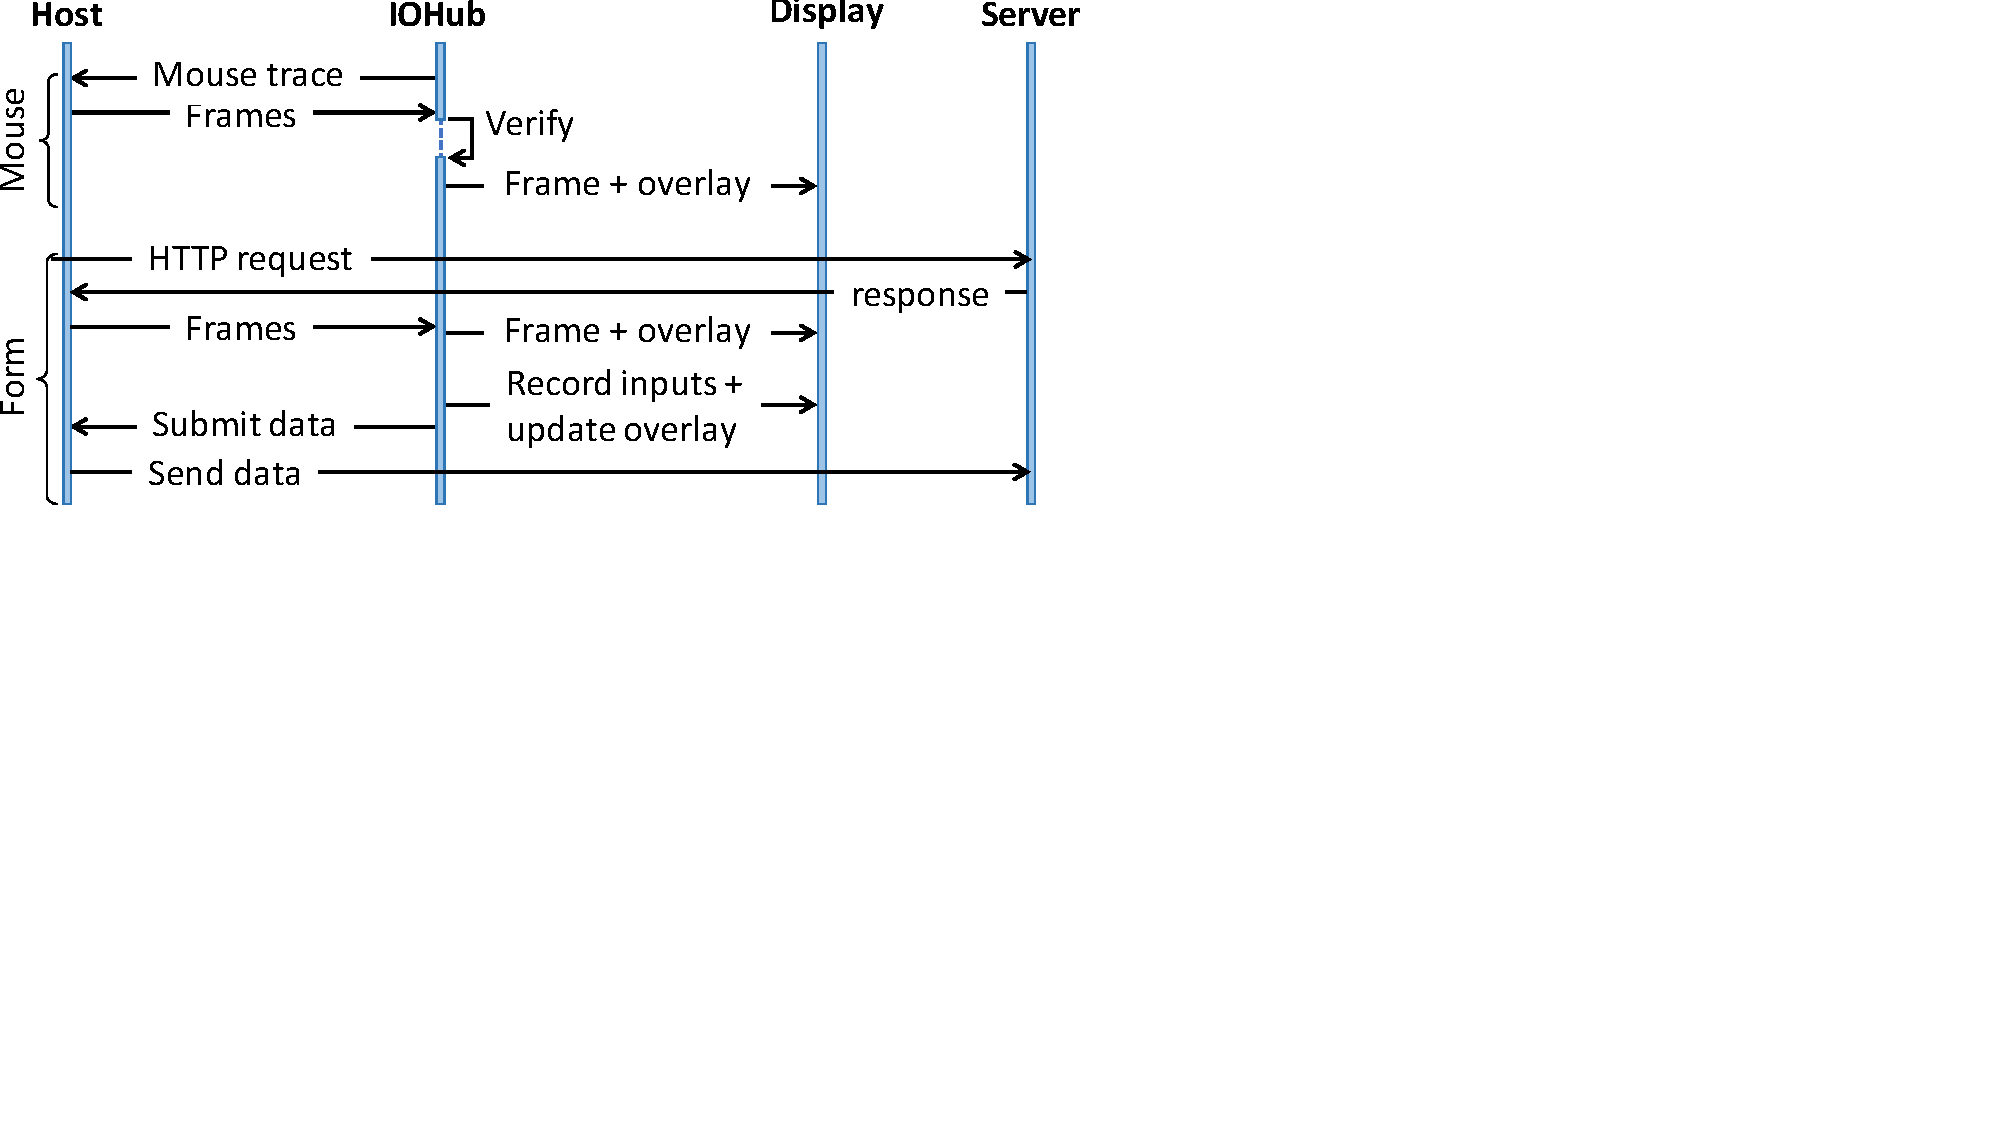
\includegraphics[trim={0 9.5cm 15cm 0}, clip, width=0.85\linewidth]{chapters/ProtectIOn/images/SequencDiagram.pdf}
\caption[Flow of the \name main protocol]{\textbf{Flow of the \name main protocol.} The figure shows the sequence of events for two example scenarios: mouse movement and filling up a web-form.}
\spacesave
\label{fig:sequence}
\centering
\end{figure}


\subsection{Protected User Interaction}
\label{sec:systemDesign:commit}

When the user finishes providing her input via input devices (mouse and keyboard), the \device sends these values (with signature to ensure integrity) to the remote server. Sending these signed input values to the server requires an upstream channel from the \device to the server. 


\subsubsection{Upstream channel}\label{sec:systemDesign:commit:upload} 
The data from the \device to the remote server is transmitted using the \name JavaScript snippet as a helper. 
%The \name JavaScript snippet uses a hidden text field to accept data coming from the \device. 
The \device emulates itself as a composite human interface device (HID) when it is connected to the host. The \device emulates keystrokes that transmit encoded data to the \name JavaScript snippet, which then forwards them to the remote server.


\subsubsection{Sending input data} Figure~\ref{fig:sequence} depicts the user interactions in a sequence diagram. The user input transmission procedure is illustrated in Figure~\ref{fig:transformation}. This has two phases: \emph{record} and \emph{transmit} as described in the following:

\begin{enumerate}
\item \textbf{Record.} After the UI elements are correctly overlaid on the screen, the users can interact with these UI elements. The user interaction with the overlaid UI element is no different than a standard UI. The UI specification encodes the behavior of all generated UI elements, making the \device aware of the semantics of the UI objects. E.g., when a user selects a text box and types on with her keyboard, the \device intercepts all keystrokes and renders the characters on the overlay.
When user enters input data in the rendered overlay UI elements (such as textbox, button, slider, radio button, etc.), the \device records that in a (key, value) pair where the key is the identifier of the UI element (\emph{id} in Specification~\ref{snippet:UISpecification}) and the value is the user provided value. The \emph{type} of the UI elements determines what information to record. For example, the \device records all keystrokes when a textbox is selected, the value corresponding to the position of the slider is recorded when the user interacts with a slider, etc. One example of the recording of the input data corresponding to the UI illustrated in Figure~\ref{fig:transformation} and Specification~\ref{snippet:UISpecification} is: 
\begin{align*}
Record = & (tb\_1, Data\_1);(tb\_2,Data\_2)
\end{align*}

\item \textbf{Transmit.} In the transmit phase, the \device waits for the user to select a UI element that has a \emph{trigger} capability, e.g., a submit button on a web-form. A trigger element can change the state of the overlaid form, e.g., submit the data of the form to the remote server or reset it. More details are provided in the implementation of \name in Section~\ref{sec:prototype:impl:qr}. When the user clicks the \emph{OK} button, the device signs $Record$ with its embedded private key. One such signed packet is also illustrated in Figure~\ref{fig:transformation}. The \device sends the signed packet to the remote server using the upstream channel.
\end{enumerate} 

%\subsubsection{\bfseries Server-side verification} \label{sec:systemDesign:commit:verification}
Upon receiving the signed input data from the \device, the remote accepts the input if the signature verification is successful. Note, if an input field is annotated as \texttt{protect=``true''}, the server does not accept any input without the \device signature. This prevents the attacker-controlled host to submit data. 


\subsubsection{Changing browser tabs or browsers}
The \device supports multiple browsing tabs across multiple browsers. The UI specification contains \emph{formId} and \emph{domain} that works as the unique identifier for a specific form served from a specific web server. The \device can maintain multiple parallel TLS connection to web servers. Depending on the observed \emph{formId} and \emph{domain} (refer to Specification~\ref{snippet:UISpecification}), the device retrieves the data that is entered by the user. This way even if the user switches tabs, the \device can still allow editing the forms across tabs.


\subsubsection{Input validation} Input validation, i.e., checking the input against a recommended input policy (e.g., regular expression) is one of the most widely used JavaScript functionalities, and it is a critical part of input integrity. The remote server sends the regular expression in the UI specification (\emph{RE} in Specification~\ref{snippet:UISpecification}) that the \device uses to validate the user input.

%\myparagraph{Sequence of Events} In the previous sections, we explain the basic components of \name. Here we summarize the overall flow of the system. The sequence diagram of \name is illustrated in Figure~\ref{fig:sequence} that shows snapshots of two example sequences: mouse movement and filling up a web-form.


\subsubsection{Fallback for legacy clients} \name is backward-compatible with the clients who do not use the \device. This is achieved by the remote server by showing a QR code briefly on the screen when the user visits the \name-enabled webpage. The \device intercepts the QR code and sends a signal to the server about its presence. In the absence of the \device, the remote server does not send the \name JS to the host that acts as a communication channel between the \device and the remote server. Note that the fallback mechanism is application-specific, and the service provider could decide if the fallback is detrimental to security.


\section{\name for IO Confidentiality}
\label{sec:confidentiality}


In the previous sections, we describe how the \name \js and the \device together ensure the integrity of the IO. We now augment the design of \name to achieve IO confidentiality alongside the IO integrity. One of the major components for achieving IO confidentiality is to establish a secure channel (i.e., a \tls channel) between the remote server and the \device. \tls ensures that the untrusted host does not read or modify any data exchanged between the user and the remote server.


\subsection{IO Operations}
\label{sec:confidentiality:io}

\lstset{language=HTML, frame=tb, caption=\textbf{Example HTML form showing encrypted UI specification. } HTML page from the remote server that contains the encrypted UI specification for IO confidentiality. , label = snippet:encryptedHTML, firstnumber =1}
\begin{figure}[t]
\small
\begin{lstlisting}[mathescape=true]
<form action="/some_action">
  Text box 1:<br>
  <input type="text" name="text_box_1">
  <br> text box 2:<br>
  <input type="text" name="text_box_2">
  <encrypted_qr><!-encrypted UI specification->
  0x4a5c4... </encrypted_qr>
  <script> [JS outputs QR code that encodes 
  encrypted specification] </script>
</form> 
\end{lstlisting}

\end{figure}



%After the server and the \device establish the \tls channel, \name is ready to provide IO confidentiality.

\subsection{Establishing TLS} The \device and the server create TLS using the public certificates. The TLS uses the emulated keystroke streams and HDMI as the upstream and downstream channels, respectively, as described in Section~\ref{sec:systemDesign}. Implementation details are provided in Section~\ref{sec:prototype:impl:tls}. 


\subsection{Output confidentiality} Output confidentiality ensures that information sent from the remote server and the visual render of the user's input is hidden from the host. To enable output confidentiality, the UI overlay mechanism that is described in Section~\ref{sec:systemDesign:transformation} is modified slightly. The difference is that the specification is not generated in the host side, but rather in the server.
%Here we \name does not require \name JS to transform all the UI elements to QR code specification. 
A small server-side module that is very similar to \name JS transforms the UI elements to the UI specification (one example is provided in Specification~\ref{snippet:UISpecification}) and encrypts it with the \tls session key. 
The encrypted specification is delivered to the client browser inside the \texttt{<encrypted\_qr>} tag in the HTML file which is then encoded (as a QR-code) by the \name JS. The \device decodes the QR code from the intercepted HDMI frames, decrypts the specification and renders the overlay accordingly. One example is provided in the HTML Snippet~\ref{snippet:encryptedHTML} with the corresponding UI illustrated in Figure~\ref{fig:activityPrivacy}. 
%The \texttt{<encrypted>} tag contains the encrypted UI specification from the server. The \name JS (inside \texttt{<script>} tag) encodes this encrypted UI specification to a QR code.
This feature of \name allows the remote server to send securely private information to the user in the presence of a compromised host, e.g., bank account statements, or any other confidential message. 


\subsection{Input Confidentiality} When the user enters her mouse pointer into the overlaid UI area, the \device stops transmitting any mouse or keyboard event to the host, making it completely oblivious of any mouse movement or keystroke during that time. 
However, the user can still see her inputs on the screen as the \device renders the plaintext character on the overlaid UI elements, therefore making them visible only to the user.
Likewise, when the user selects a UI element, for example, a radio button that is shown in Figure~\ref{fig:activityPrivacy}, the \device stores the selected value in the recorded data.
On form submission, \device encrypts the recorded data with the \tls key and sends them to the remote server.
%encrypts, signs the packets and sends it to the remote server making the input commands/values hidden from the attacker-controlled host.  

\begin{figure}[t]
\centering
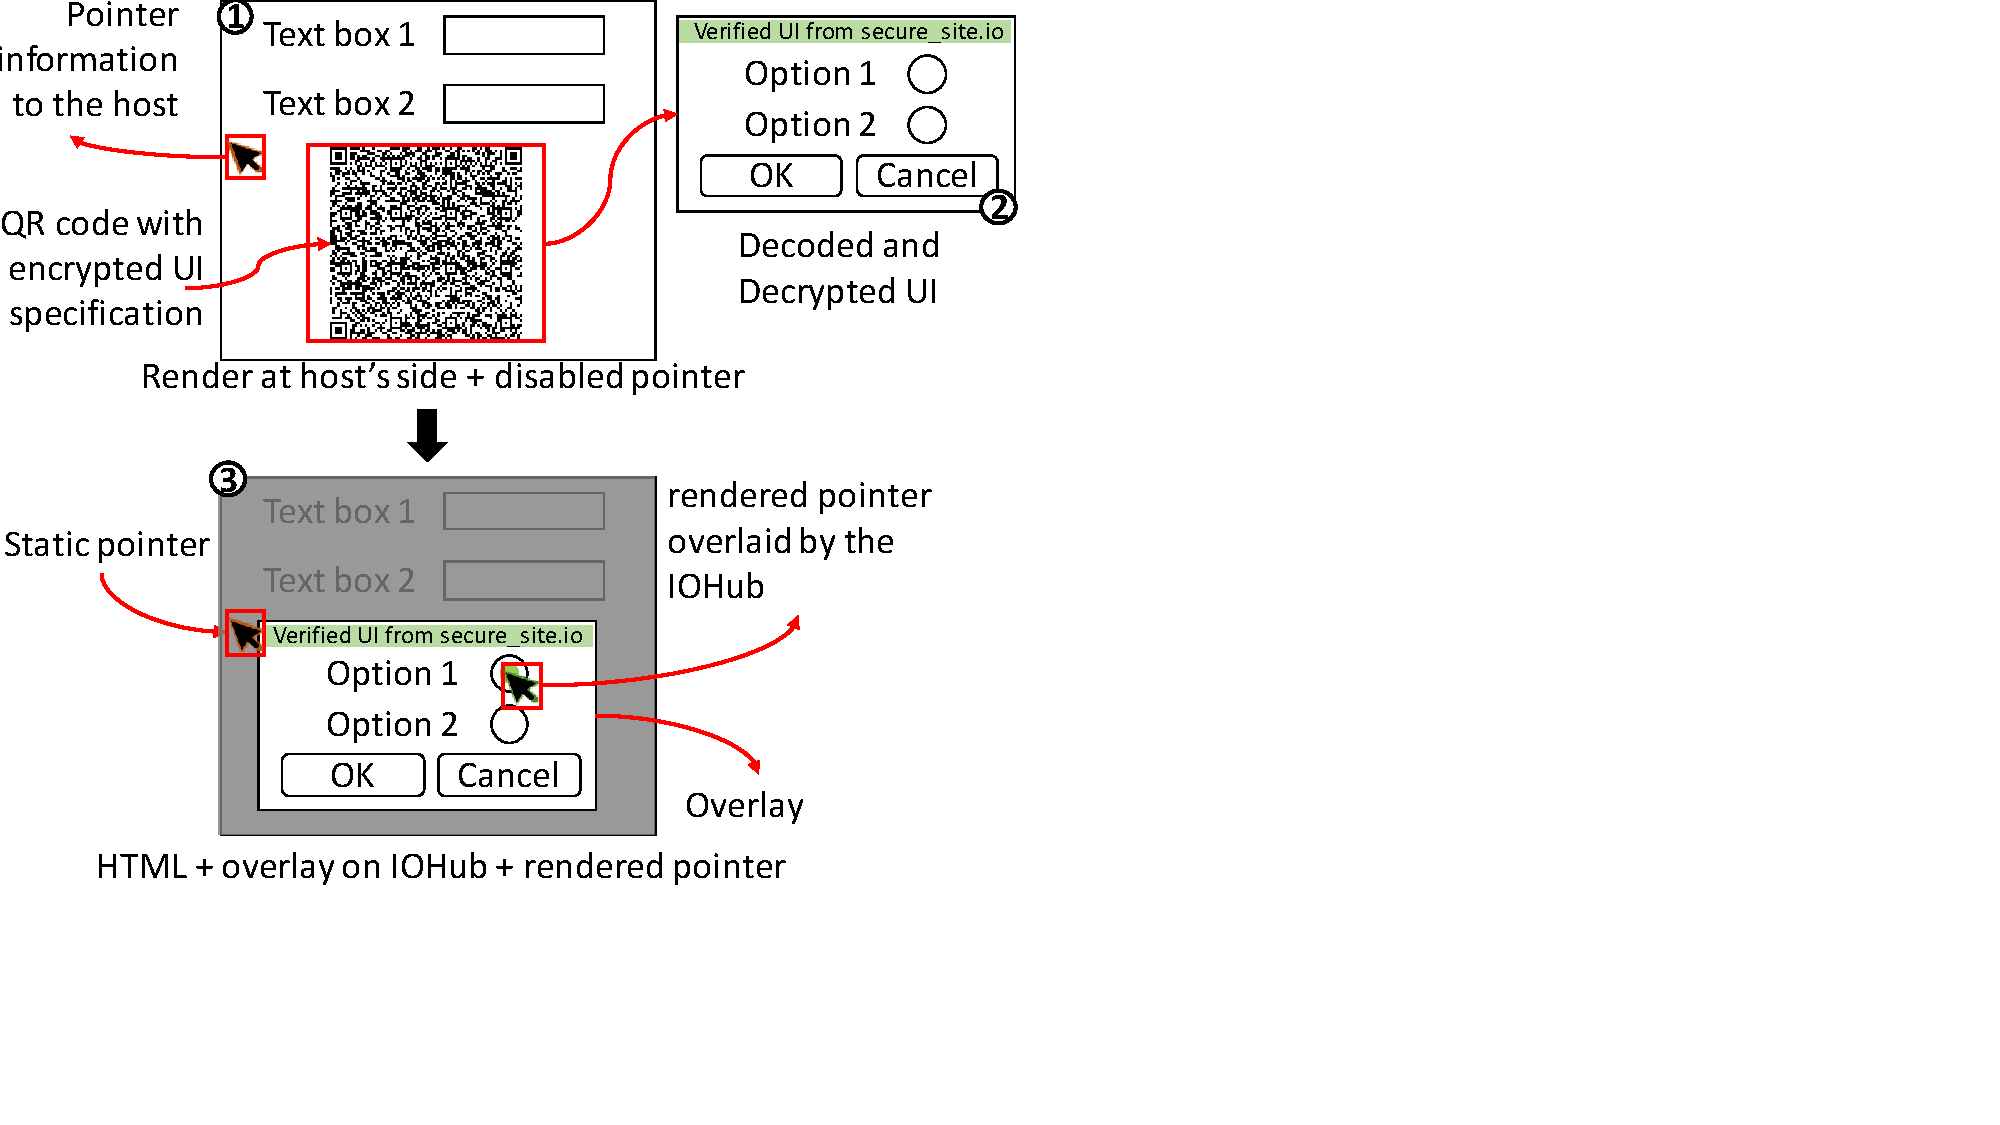
\includegraphics[trim={0 4cm 16.5cm 0}, clip, width=0.88\linewidth]{chapters/ProtectIOn/images/activityPrivacyRender.pdf}
%\caption{\textbf{\name IO confidentiality.} The figure shows how \name achieves the confidentiality of the UI elements and the mouse pointer in the presence of a compromised host. The upper screenshot shows the host's view of the display, while the lower one shows the user's view. The host can only see a QR code where the specification is encrypted by the \tls session key between the \device and the remote server. The user saw the decoded and overlaid UI objects that are retrieved from the QR code sent by the remote server (as described in Section~\ref{sec:systemDesign:transformation}).}
\caption[\name IO confidentiality]{\textbf{\name IO confidentiality.} The figure shows \one the browser render of the webpage in Specification~\ref{snippet:encryptedHTML} where the \name \js produces the encrypted QR code. \two shows the UI overlay that is decrypted and decoded by the \device. \three shows the user's view when the \device overlays the UI on the HDMI frame, and the user starts to interact with the UI.}
%\spacesave
\label{fig:activityPrivacy}
\centering
\end{figure}

\subsection{Focusing User Attention} 
\label{sec:confidentiality:SAS}

The IO confidentiality could be viewed as a similar problem to \emph{phishing} where the user provides the inputs to an attacker-generated UI (or a phishing webpage) that leaks the sensitive information. Similar to the phishing protection mechanisms, IO confidentiality requires additional attention/operations from the user. Secure Attention Sequence (SAS) is a sequence of trustworthy actions (such as keystrokes \texttt{Ctrl+Alt+Del} in Windows) executed by the user. SAS prevents an untrusted system from triggering an event that is otherwise sensitive to the user. Note that SAS is a well-researched topic in the context of UI/UX design. \name adapts an off-the-shelf SAS mechanism that provides a visual aid for the user to distinguish overlaid UI and the mouse pointer location. SAS is crucial for IO confidentiality as the untrusted host can trick the user into inputting her sensitive information on a forged form. Hence, the user needs to remember the SAS to distinguish \device generated UIs from host generated UIs. Note that the automated activation is insufficient as at any given time, the host can maliciously emulate the automated activation to trick the user into providing sensitive information to an illegitimate UI.

Note that SAS is one of many ways to inform the user securely about the trusted overlay on the screen generated by the \device. Evaluation of the effectiveness of SAS over other attention focusing mechanisms is out-of-scope of this paper. Hence, \name uses SAS as an example of the attention focusing mechanism for confidentiality. In principle, \name could be integrated with other proposed approaches such as security indicators, or secret images~\cite{6894474,Marforio2016}.


\subsection{UI protection profile} The remote server can set a configurable UI protection profile per overlaid protected UI (i.e., QR code). The protection policy is defined in the \texttt{SAS} attribute in the example specification provided in Specification~\ref{snippet:UISpecification}. The policy dictates how the UI would respond to the SAS provided by the user. By default, the overlaid UI is locked from the user and requires the SAS keystroke from the user to unlock the sensitive UI. This information is overlaid on the UI to remind the user to execute it. One example UI protection policy could be \texttt{5:LB} (refer to Specification~\ref{snippet:UISpecification}), which denotes \device invokes a lightbox on the HDMI frames except for the UI overlay and the mouse pointer overlay for a cool-down period of $5$ seconds. The form remains locked for this cool-down period.

The design of the \name system is independent of the secure attention sequence (SAS) value. In principle, each issuer that deploys \device devices to users (see Section~\ref{sec:approach:systemAttackerModel}) could define its own custom SAS and configure the deployed \device devices to intercept that key sequence. Our recommendation, however, is that the \device issuers follow established platform-specific SAS values. For example, if a \device device is issued for the purposes of protecting user interactions on a  Windows platform, we recommend that the device issuer pre-configures the \device to intercept the Windows-specific \texttt{Ctr+Alt+Del} sequence. Similarly, if a \device device is deployed to be used on another OS, it should be pre-configured to intercept the SAS sequence commonly used on that platform. (In cases where the same \device device would be used on multiple different platforms, it could be either configured to intercept multiple SAS values or it could use a single SAS value that the issuer needs to communicate to its user.)
%or SAS to prevent the attacker from putting a different SAS instruction on the screen. The SAS keystroke is first intercepted by the \device that checks for the QR code on the HDMI stream.}

%One example policy could be \texttt{Ctrl+d:5}, which denotes that the user needs to press key `\texttt{Ctrl+d}' to unlock the UI overlay. Pressing this key also triggers the \device to blackout the HDMI frames except for the UI overlay and the mouse pointer overlay for a specified time (here for $5$ seconds). 



\section{Security Analysis}
\label{sec:securityAnalysis}

In this section, we will informally analyze the security of \name. We divide the security analysis into two parts based on two security properties: interity and confidentiality.

\subsection{Integrity}
\label{sec:securityAnalysis:integrity}

First we look into the integrity property.

\myparagraph{Modifying IO operations} As only the \device can interact with the overlaid UI, the attacker can not manipulate the IO operations with the overlaid UI. Moreover, the attacker cannot submit arbitrary data to the remote server because the latter accepts only inputs signed by the \device.


\myparagraph{Early form submission} This attack is not possible as the input devices (both mouse and keyboard) are connected to the \device, and only the \device can interact with the overlaid UI. This makes it impossible for the attacker to emulate a click on the overlaid part of the screen.  


\myparagraph{Attack on the mouse pointer tracking and overlay} 
The attacker may try to defeat the \name pointer tracking and overlay mechanism described in Section~\ref{sec:systemDesign:analysis} by introducing a malicious pointer that is visually more appealing to the user. Note that the \device overlaid mouse pointer is prominent and hard to miss. One can visualize it as an arms race between the attacker and the \device to grab the user's attention. We argue that this is a suboptimal strategy for the attacker as both of the pointers will be visible on the screen that causes suspicion to the user. Also, when the real mouse pointer enters the overlaid area, the untrusted part, including the malicious mouse pointer, will be hidden by the focusing mechanism. Hence, we can conclude that executing clickjacking-like attacks is not possible in \name.


\myparagraph{Replay attack} The remote server adds a random identifier (\texttt{id}) in the form specification alongside the signature. With this identifier, the server keeps track of the user input. When the server receives a form submission data, it first checks if the user submitted with the same identifier sent by the server. Otherwise, the server rejects the data. 


\myparagraph{Not rendering QR code} The host may deny sending the QR code over the HDMI channel. We consider this to be a denial of service and does not compromise the integrity of the IO data. 


\myparagraph{Redirection} The attacker could redirect the user to a phishing website that renders visually identical UI to that of the legitimate website. A redirection attack cannot break the integrity of the input because a legitimate remote server always requires the signed input from the user. Without a valid signed specification, the \device never renders an overlay or sign any input. 

\myparagraph{Malicious instruction on the screen} The attacker may put a malicious instruction/label on the untrusted part of the screen to influence user inputs. However, when the user starts interacting with the overlaid UI, the default focusing mechanism (Lightbox) highlights only the secure UI and hides the rest of the screen. 
%The user attention focusing mechanisms enable the user to distinguish the trusted part of the screen from the untrusted part.


\myparagraph{Replication of Lightbox} The attacker can replicate the lightbox on any part of the screen. However, this does not compromise the integrity of the input as the legitimate remote server only accepts signed input from the \device. 


\myparagraph{Multiple HIDs} The attacker can emulate multiple HIDs to avoid the tracking of the mouse pointer. However, this attack is ineffective as the \device only tracks the mouse pointer that is connected to it (over USB interface). 


\myparagraph{BadUSB} BadUSB~\cite{badUSB} is out-of-scope of this paper as in the attacker model (Section~\ref{sec:approach:systemAttackerModel}), we assume that all the IO devices that are connected to the \device are trusted.

\myparagraph{Mouse acceleration/updates} The attacker can change the mouse acceleration or provide erratic mouse updates on the screen. Such manipulations only cause the \device to lose track of the mouse pointer and stop relaying the mouse signal to the host altogether. The \device uses the acceleration parameters from the default \texttt{libUSB} driver to cope with the mouse acceleration. Hence, such manipulation does not affect security.

\myparagraph{Malicious QR codes} The attacker may put fake QR codes on the webpage. Note that the \device verifies the signature from the HTML forms to check the integrity using the pre-configured or white-listed server certificate. This way, the \device does not render any overlays from malicious QR codes.


\subsection{Confidentiality}
\label{sec:securityAnalysis:confidentiality}

\myparagraph{Redirection} The attacker could redirect the user to a phishing website that renders visually identical UI to that of the legitimate website. Redirection compromises the confidentiality of user inputs only when the user does not trigger the SAS mechanism. The \device is only activated when it detects specifications signed from the whitelisted (maintained in the memory) servers.
%Note that the \device contains a whitelist of the remote server addresses and their corresponding certificates. The \device is only activated when it detects specifications signed from the whitelisted servers.
%as the confidentiality of inputs requires the user to manually trigger the SAS to detect any sensitive UI elements that are overlaid by the \device.


\myparagraph{Fake SAS instructions} The attacker may put fake instructions on the screen that attempt to trick the user into typing a false SAS sequence and then revealing her sensitive information to the attacker. This attack is not possible as long as the user follows the instructions it received from the issuer of the \device and only types in secrets after using the correct SAS value (such as \texttt{Ctr+Alt+Del}). Recall from Section~\ref{sec:confidentiality:SAS} that the SAS value is defined by the issuer of the \device and that the SAS keystrokes are always first intercepted by the \device. (The user is expected to trigger the SAS only when there exists a QR code on the screen that is correctly signed by the remote server. In case there is no QR code or a malformed QR code on the screen, the \device warns the user.)


\myparagraph{Side-channel leakages} Even though, the \device ensures that no mouse or keyboard event arrives at the untrusted host when the user executes some operation over the overlaid UI, one can not rule out all side-channel leakages. Depending on the application, the amount of time that the user spends or the entry/exit position of the mouse pointer may reveal some information to the attacker. 
\device could allow the remote server to specify additional policies in the specification to prevent such side-channel attacks, e.g., a minimum amount of time that the device should not forward any event to the host after the user enters the overlay. We leave as future work defining such policies and integrating them on \name.
%However, for fixed-length inputs such as the pin codes or credit card details, do not leak any information about the input.


\myparagraph{Mode Switching} The host could remove the QR code when the user is typing confidential data in the sensitive form. The absence of the QR code makes the \device to assume that the secure session has ended, and the \device forwards the plaintext keystrokes and mouse movement to the host. To prevent the leakage of the input data, the \device continues to overlay and operate on the overlay until the user clicks submit or cancel (or any UI element that has a \texttt{trigger}  capability). This way, the \device locks the UI from the attacker until the user finishes her session.

\subsection{Attacks toward \device} 
\label{sec:securityAnalysis:device}

In \name trust model, we assume that the \device is trusted. However, in the real-world, embedded systems are often vulnerable to attacks as the attacker can use the connection interfaces to reprogram the \device. It is also possible to develop the \device using formally verified languages such as embedded Rust. However, we consider making a security-hardened \device is engineering intensive and out-of-scope of this paper. 


\myparagraph{Downgrade attack} The host can block the initial QR code from the server to the \device. By doing so, the host forces the server to downgrade the security of the webpage, i.e., not serving the \name JS. For integrity, this is not a security threat as the server does not accept any input from the host that is not signed by the \device. Hence, the downgrade attack works as a denial of service, which is out-of-scope of this paper.
%The fallback mechanism, i.e., the case where the user does not have the \device, is outside the scope of this work because it is specific to the policy of service providers. E.g., a bank could issue a new \device for the user, while an online shopping site could allow the user to enroll a new \device or allow access only to nonsensitive functionalities. 


\subsection{Proof for IO Integrity}
\label{sec:securityAnalysis:proof}

In this section, first, we provide a formal proof of the following property: \emph{without protecting both input and output integrity, none of them can be achieved}. 


%\subsection{Interaction Protocol} 
%\label{appendix:security:protocol}

\myparagraph{Interaction protocol}

To simplify the proof, we model the interaction between the user, the host, and the remote server as a finite state automaton (FSA).
The interactions between the server (\server), the user (\user) and host (\host) are depicted in the FSA in Figure~\ref{fig:fsm}.

\begin{figure}[h!]
\begin{center}
\begin{tikzpicture}[shorten >=1pt,node distance=3cm,on grid,auto]
  \tikzstyle{every state}=[fill={rgb:black,1;white,10}]

    \node[state,initial]   (q_1)                    {\user};
    \node[state] (q_2)  [right of=q_1]    			{\host};
    \node[state,accepting]           (q_3)  [right of=q_2]    {\server};

    \path[->]
    (q_2) edge [bend left]  node {$[m']$}    (q_1)
    (q_1) edge [bend left]  node {$(I,[m'])$}    (q_2)
    (q_2) edge [bend left]  node {$(I,[m'])$}    (q_3)
    (q_3) edge [bend left]  node {$m$}    (q_2);
\end{tikzpicture}
\end{center}
\caption[\name protocol FSM]{Finite state machine that depicts the interaction between the user (\user), host (\host) and the server (\server).}
\label{fig:fsm}
\end{figure}


% \begin{figure}[h!]
% \begin{center}
% \begin{tikzpicture}[scale=0.15]
% \tikzstyle{every node}+=[inner sep=0pt]
% \draw [black] (66,-23.1) circle (3);
% \draw (66,-23.1) node {\server};
% \draw [black] (66,-23.1) circle (2.4);
% \draw [black] (45.2,-23.1) circle (3);
% \draw (45.2,-23.1) node {\host};
% \draw [black] (26.9,-23.1) circle (3);
% \draw (26.9,-23.1) node {\user};
% \draw [black] (47.743,-21.516) arc (116.95563:63.04437:17.332);
% \fill [black] (47.74,-21.52) -- (48.68,-21.6) -- (48.23,-20.71);
% \draw (55.6,-19.13) node [above] {$m$};
% \draw [black] (29.352,-21.382) arc (118.8302:61.1698:13.89);
% \fill [black] (29.35,-21.38) -- (30.29,-21.43) -- (29.81,-20.56);
% \draw (36.05,-19.16) node [above] {$[m']$};
% \draw [black] (42.565,-24.526) arc (-66.78269:-113.21731:16.527);
% \fill [black] (42.57,-24.53) -- (41.63,-24.38) -- (42.03,-25.3);
% \draw (36.05,-26.36) node [below] {$(I,[m'])$};
% \draw [black] (63.369,-24.535) arc (-65.91058:-114.08942:19.034);
% \fill [black] (63.37,-24.53) -- (62.43,-24.4) -- (62.84,-25.32);
% \draw (55.6,-26.69) node [below] {$(I,[m'])$};
% \end{tikzpicture}
% \end{center}
% \caption[\name protocol FSM]{Finite state machine that depicts the interaction between the user (\user), host (\host) and the server (\server).}
% \label{fig:fsm}
% \end{figure}

We consider a setting where the user \user interacts with \server over browser through web UI. Hence we assume that all the messages ($m$ or $m'$) exchanged between the user \user, host \host and server \server is HTTP request and response payload. The HTTP response payloads (originating from \server) contains HTML, JavaScript, CSS and other data to construct the webpage at the host's browser. The protocol starts with \user sending an initial request to \server that is delivered through \host. We denote $[m]$ to be the render of $m$ by the \host, i.e, graphical render of the webpage ($m$) on the host's display. In this initial stage consider $[m'] = \phi$. Upon receiving the initial request, the server \server replies with a message $m$ to \host. As \host is malicious, it can transform $m$ to $m'$. Note that this transformation from the message to render to the user's display is a public knowledge and is deterministic. Hence, for a message $m'$, where $m\neq m'$, then given the corresponding renders $[m']$ and $[m]$, \server can determine that $[m]\neq [m']$. We denote the user input to be $I$, which corresponds to a specific $[m]$. 
%Note that the communication channel between \server to \user is neither authenticated, neither confidential. But the communication channel from \user and \server is authenticated. 
In this model, we simplify the user input by assuming that the \user only provides an input $I$ only after observing a message transformation $[m]$. The user provides both her input $I$ and transformation $[m']$ observed by her to \host. The interaction loop between \host and \user can continue until \user finishes her input. After every input \host hands over new message transformation to \user (either result of the input or new message from \server or both). This simulates the changes in the web UI when the user starts interact with it e.g., input feedback. Once the user provides all her inputs, \host send the sequence of pairs $(I, [m'])$ to \server.

To smmarize the interaction protocol above, we define these two mappings as the following:

\begin{align*}
\texttt{Input()}&:[m]\rightarrow I \\
\texttt{Transform()}&:m,I\rightarrow [m'],\ \exists i\in I:i=\phi
\end{align*}
Both of them are \emph{bijective}.

One trace of the protocol transcript mentioned above is depicted in Figure~\ref{fig:protocol}. As described in the FSM (refer to Figure~\ref{fig:fsm}), \server receives a trace of message transformations $([m']_1,[m']_2,\ldots,[m']_n)$ and corresponding inputs ($I_1,I_2,\ldots,I_n$). From these traces \server could determine of all the $[m']_i$ are in proper form by verifying if $[m]_i=[m']_i$.

Given the interaction protocol, we can now formally define the definitions in this chapters such as the input intergity and output intergerity as the following:

\begin{figure}[t]
\begin{center}
\tikzset{
  every picture/.append style={
    transform shape,
    scale=1
  }
 }
\begin{sequencediagram}
\newinst{u}{\user}
\newinst[3]{h}{\host}
\newinst[3]{s}{\server}
\mess{s}{$m$}{h}
\mess{h}{$[m']_1$}{u}
\mess{u}{$I_1,[m']_1$}{h}
%\mess{h}{$[m']_2$}{u}
%\mess{u}{$I_2,[m']_2$}{h}
\mess{h}{...}{u}
\mess{u}{...}{h}
\mess{h}{$[m']_n$}{u}
\mess{u}{$I_n,[m']_n$}{h}
\mess{h}{$I_1,I_2,...,I_n$}{s}
\mess{h}{$[m']_1,[m']_2,...,[m']_n$}{s}
\end{sequencediagram}
\end{center}
\caption[\name protocol transcript]{Protocol transcript between the \server, \user and \host that shows one trace from the FSM depicted in Figure~\ref{fig:fsm}.}
\label{fig:protocol}
\end{figure}


\begin{definition}{\textbf{Input integrity}}
\label{def:inputIntegrity}
Assume that \server handed a message $m$ to \host where the proper message transformation is $[m]$. The host changes the message transformation to $[m']$ where $[m']\neq [m]$. We also define correct \user input to be $I$ when \host sends a correct message transformation $[m]$ to \user. We define input integrity as the property where the \server does not accept input $I'$ where $I'\neq I$from \user if the \host changes the message transformation.
\end{definition}

\begin{definition}{\textbf{Output integrity}}
\label{def:outputIntegrity}
Assume that \server handed a message $m$ to \host where the proper message transformation is $[m]$. Output integrity defines that in all circumstances, \user receives the correct message transformation $[m]$ from \host.
\end{definition}

\myparagraph{Verification process} After receiving all the traces, \server checks $\forall i=1\ldots n$, if $$[m']_i =^? \texttt{Transform}(m_{i-1}, I_{i-1})$$ where $I_0=\phi$.

\begin{lemma}
\label{theorem:th1}
If \user does not send all the transformations till $[m']_i$ corresponding to the input $I_i$, input integrity can not be achieved. 
\end{lemma}

\begin{proof}
If \user does not attach all the transformation till $[m']_i$, i.e., $$[m']_1, [m']_2, \ldots, [m']_{x+1}, [m']_x, [m']_{x-1}, \ldots, [m']_{i-1}, [m']_i$$  corresponding to inputs $I_1, I_2,\ldots, I_{x-1}, I_x, I_{x-1}, \ldots, I_{i-1}, I_i$, then the server can not verify all the transformations corresponding to the input. \host could modify a specific $[m]_x$ to influence \user input. Hence, the following verification will be missing:
$$[m']_x=^?\texttt{Transform}({m'}_{x-1}, I'_{x-1})$$
Where the \host changes message $m$ to $m'$ influence the the user to change her input from $I_{x-1}$ to $I_{x-1}$. Hence input integrity can not be achieved.
\end{proof}

\begin{lemma}
\label{theorem:th2}
If the channel from \user and \server is not authenticated, input integrity is not achievable. But the channel from \server to \user does not require to be secure as long a \user provides the message transformation $[m']_i$ corresponding to every input $I_i$.
\end{lemma}

\begin{proof}
The proof is trivial. If the channel from \user to \server is not authenticated, any input provided by \user can be manipulated by \host without a trace. Hence input integrity is not achievable. As long as \user sends message transformation along with the input, a manipulated message transformation bt \host would be detectable by \server (see Lemma~\ref{theorem:th1}).
\end{proof}

\begin{lemma}
\label{theorem:th3}
Ensuring output integrity also ensures input integrity provided there is an authenticated channel from \user to \server.
\end{lemma}

\begin{proof}
This proof is also trivial. As we describe in the Definition~\ref{def:inputIntegrity} and~\ref{def:outputIntegrity}, if all the message transform from \host $[m']=[m]$, and \host always executes \texttt{Transform()} properly, the input integrity is preserved. As \name ensures output integrity and all the input from the user is signed by the \device, \name preserves input integrity. 
\end{proof}


Similarly, we can also prove the following property: \emph{If not all the modalities of inputs are secured simultaneously, none of them can be fully secured.}

This is a general case for the proof that is described previously. We can modify the \texttt{Input} and \texttt{Transform} function to handle multiple modalities of input. 

\begin{align*}
\texttt{Input()}&:[m]\rightarrow I^1, I^2, \ldots, I^T (I^{1,\ldots,T}\text{T modalities of input}) \\
\texttt{Transform()}&:m,I^1,\ldots, I^T \rightarrow [m'],\ \exists i^t\in I^T, \forall t \in T :i=\phi
\end{align*}

Hence the verification process at the server side will be changed as the following:

\myparagraph{Verification process} After receiving all the traces (of input and message renders), \server checks $\forall i=1\ldots n$, if 
$$[m']_i =^? \texttt{Transform}(m_{i-1}, I^1_{i-1},\ldots, I^T_{i-1})$$ 

where $I_0=\phi$. If any of the input modality is missing from the trace, the server cannot verify the input integrity. 
\section{\name Prototype}
\label{sec:prototype}

In this section we provide an overview of our \name prototype implementation.

\begin{figure*}[!htpb]
    \begin{center}
        \begin{subfigure}{\textwidth}
        \centering
            %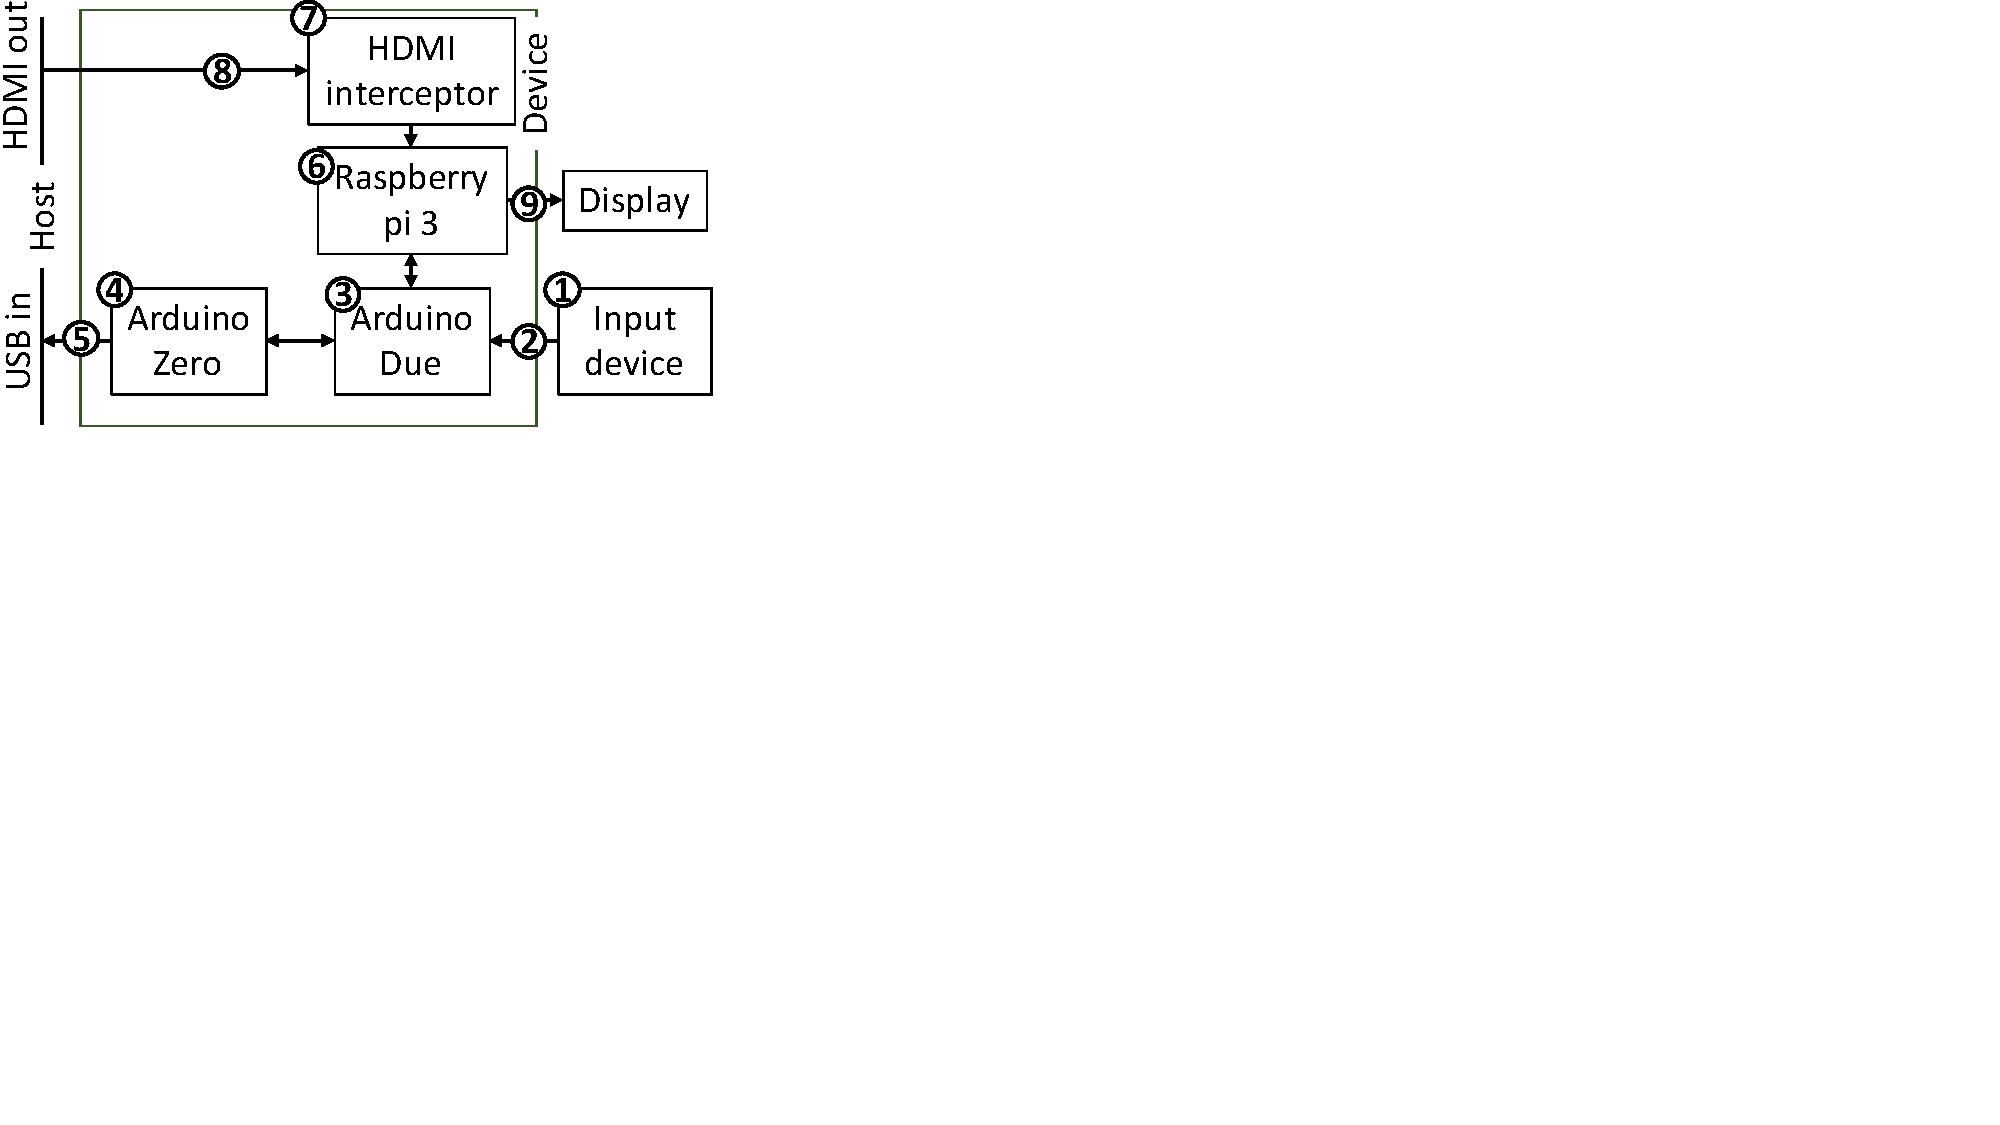
\includegraphics[trim={0 12cm 21.7cm 0}, clip, scale=0.45]{setUpBlock.pdf}
            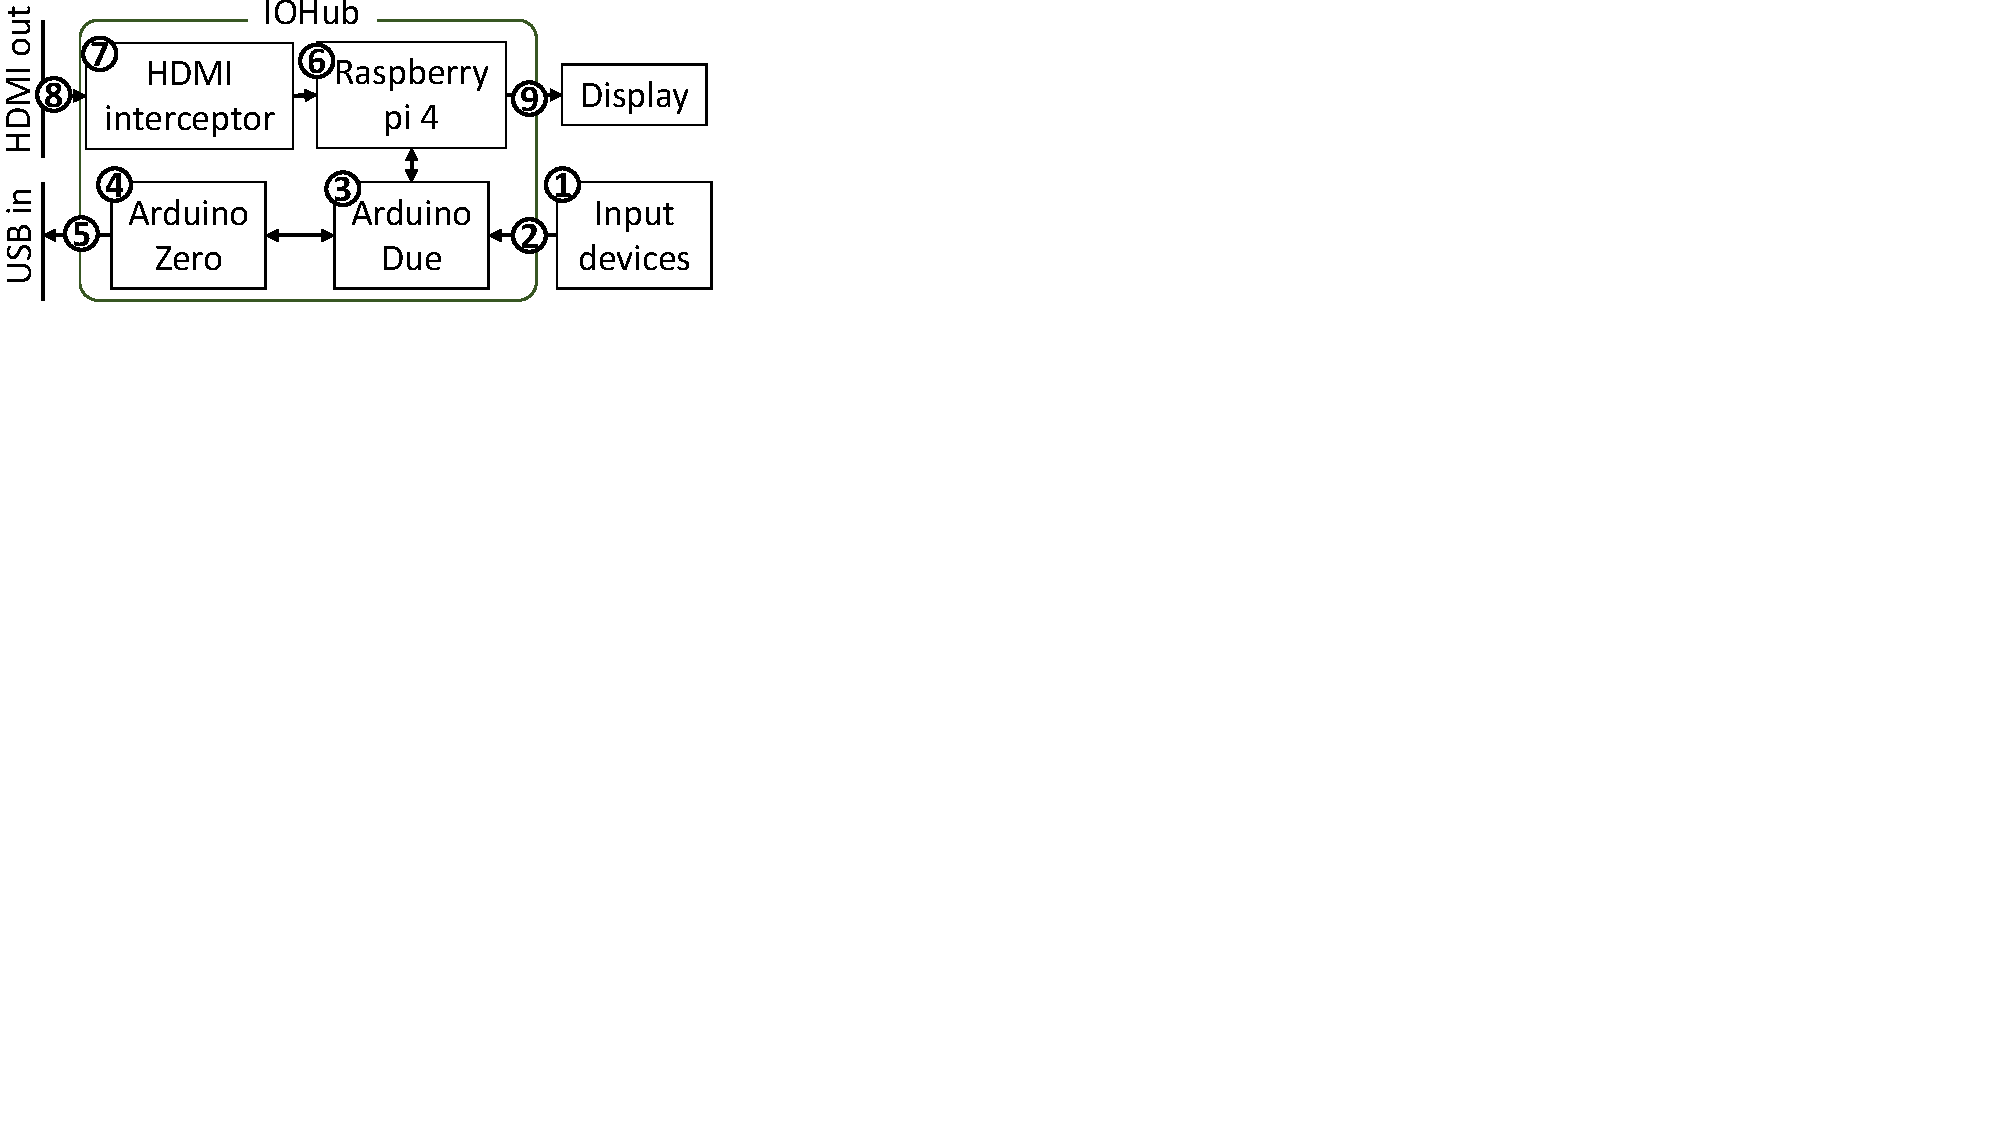
\includegraphics[trim={0 13.7cm 21.7cm 0}, clip, scale=0.5]{chapters/ProtectIOn/images/setUpBlock_1.pdf}
            \caption{The figure shows the basic components and connections between them in our \name \device prototype. \texttt{USB in} and \texttt{HDMI out} are the connection interfaced between the \device and the host platform.}
            \label{fig:prototypeArch}    
        \end{subfigure}
    \end{center}
    
    %\vspace{1em} 
    
    \begin{center}
        \begin{subfigure}{\textwidth}
        \centering
        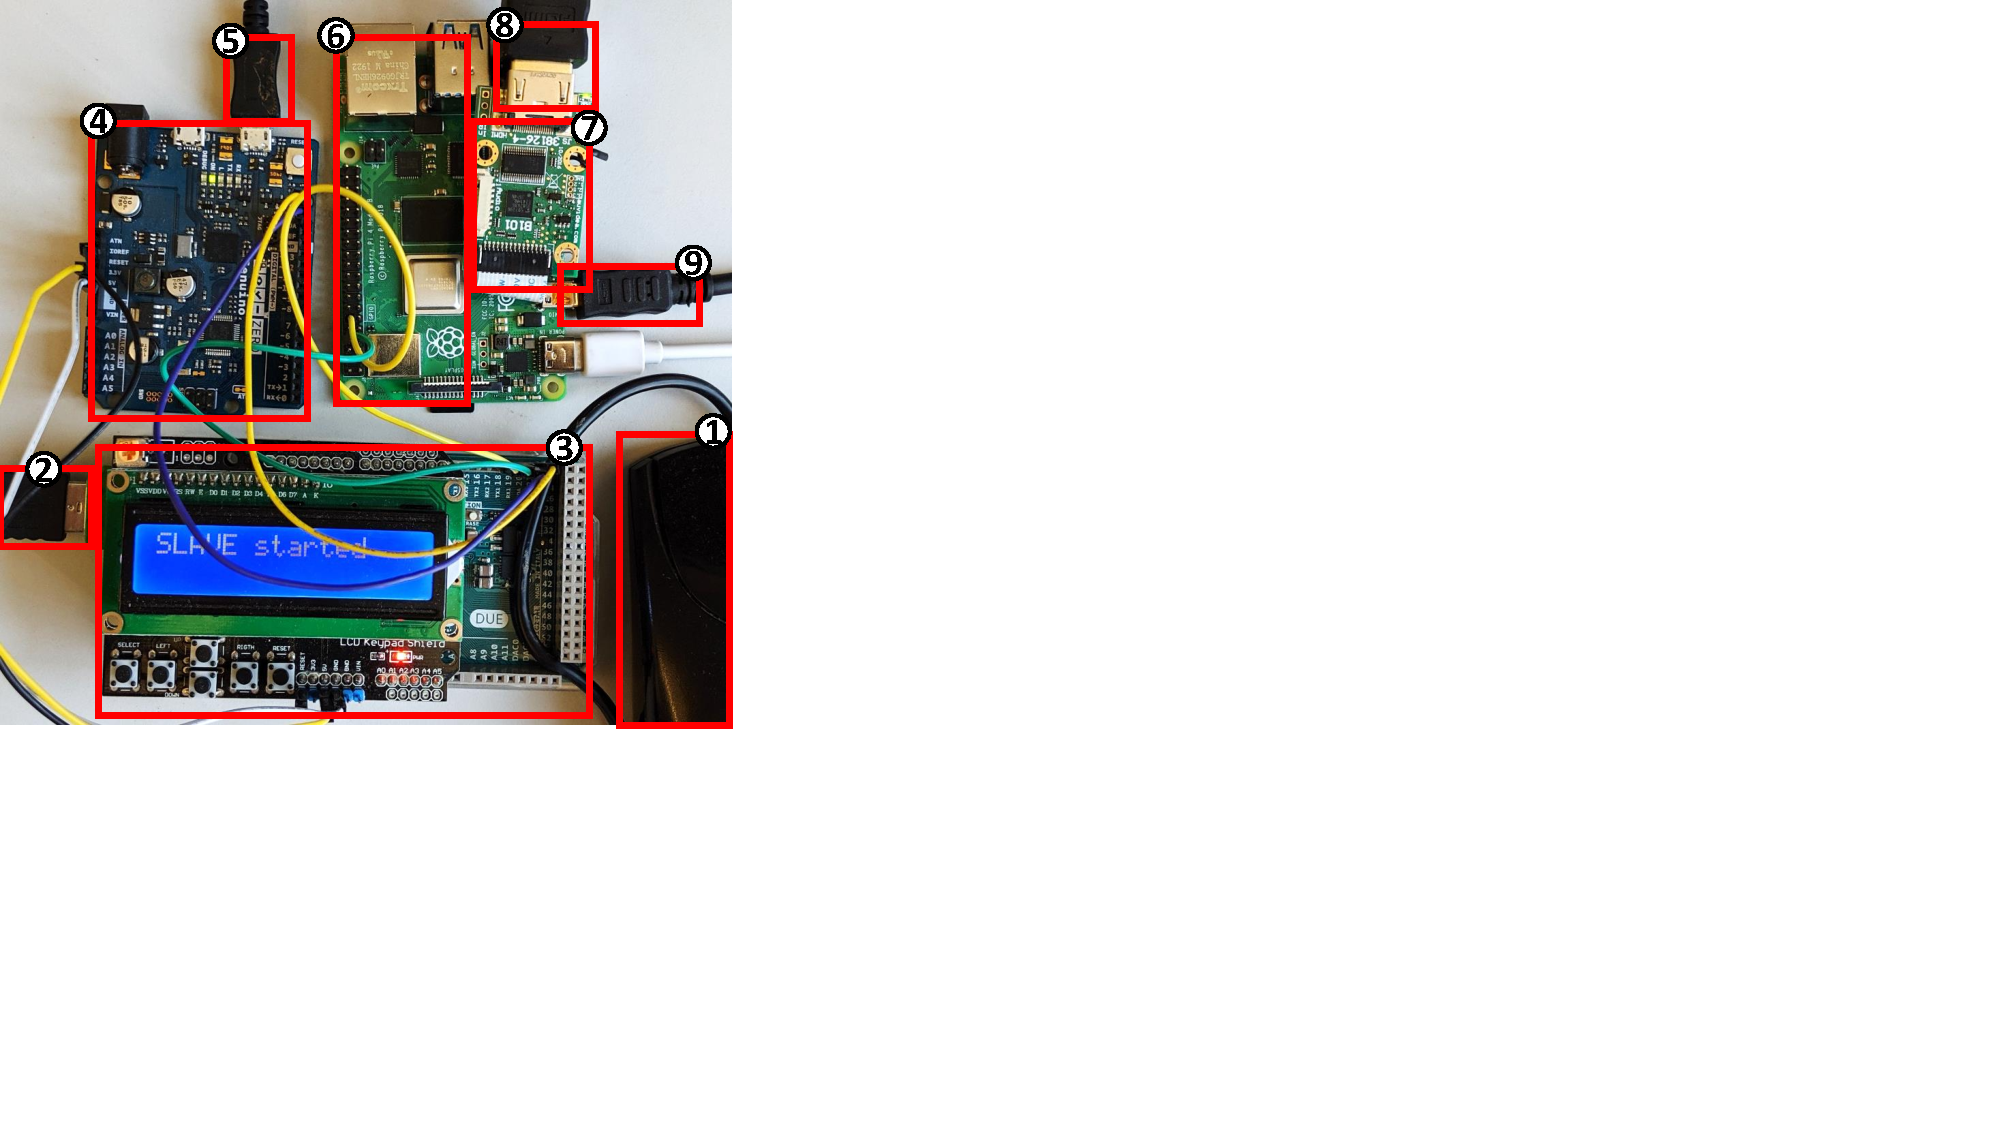
\includegraphics[trim={0 6.6cm 21.5cm 0}, clip, scale=0.55]{chapters/ProtectIOn/images/setUp_1.pdf}
        \caption{\name \device prototype uses Arduino Due and Zero microcontroller board and a Raspberry Pi 4 SBC. The highlighted numbers correspond to the labels in Figure~\ref{fig:prototypeArch}.}
        \label{fig:prototype_protection}
    \end{subfigure}
    \end{center}
   
    \caption[\name prototype]{\textbf{\name prototype}. Figure~\ref{fig:prototypeArch} and~\ref{fig:prototype_protection} shows the schematic and a photo of the  \name \device prototype respectively.} 
    \label{fig:prototypeAll}
\end{figure*}


\subsection{Setup} Here, we describe our prototype implementation of \name as an auxiliary device. Figure~\ref{fig:prototypeAll} depicts the \name prototype in two parts: Figure~\ref{fig:prototypeArch} shows the block diagram of our prototype with various components and connections, and Figure~\ref{fig:prototype_protection} shows a photo of the actual prototype that highlights all the components described in the block diagram. The prototype \device is connected to a desktop computer with 3.40 GHz Intel Core i7-6700 processor with 8 GB RAM running Ubuntu 18.04.2 LTS. The \device uses off-the-shelf devices and has the following components (we use the same numbering as shown in Figure~\ref{fig:prototypeArch} and Figure~\ref{fig:prototype_protection}):

\begin{enumerate}
 
  \item \textbf{Computing component.} We use a Raspberry Pi 4 (\six) to implement the computing component that executes all the \device logic that includes analyzing the HDMI frames, rendering the overlays, executing the \tls protocol, etc. One could use an ASIC to further improve the performance and reduce the code base of the component. The Pi is connected to the display over HDMI (\nine) interface. The code base of the Pi primarily consists of Python and Java.
  
  \item \textbf{Input interceptor.} The input interceptor is composed of an Arduino Due (\three) and an Arduino Zero (\four) that is connected to the input device over \usb (\two) interface. The input interceptor has a \usb out interface that connects to the host (\five) that relays all the user inputs to the host. 

  \item \textbf{HDMI interceptor.} The HDMI interceptor (\seven) is implemented using a B101 HDMI to CSI-2 Bridge~\cite{b101} that takes the HDMI channel (\eight) from the host and convert it to the camera input signal to the Raspberry Pi 4.  
 
\end{enumerate}

\subsection{Implementation of \name Components}
\label{appendix:implementation}


In the following, we provide the implementation details of the \name components presented in the previous sections. 

\subsection{QR code generation \& UI specification}
\label{sec:prototype:impl:qr}
%
QR code generation phase is executed by \name JS that transforms the UI elements of a sensitive web form to a UI specification encoded in a QR code (we use QRCode.js, a \js library to produce QR codes). Section~\ref{sec:systemDesign:transformation} provides the high-level concept of generating the QR code from the webpage UI elements. UI elements that require IO integrity protection can be marked by the developers in the \html source. As illustrated in Figure~\ref{fig:transformation}, the \html UI elements: `\texttt{Sensitive field 1}' and `\texttt{Sensitive field 2}' have the additional attribute \texttt{protect=``true''}. %(one concrete example is illustrated in Figure~\ref{fig:transformation}). 

The \name JS iterates through the HTML elements that have the \texttt{protect} attribute enabled and extracts the information such as the name of the label or the type of the UI element. \device uses preloaded size parameters to specify the size of a text field, button, etc. in case the size is not explicitly mentioned in the HTML source. One important attribute for a UI element in the specification is the \texttt{trigger}. For example, in Specification~\ref{snippet:UISpecification}, the \texttt{OK} and the \texttt{cancel} buttons have an attribute \texttt{trigger}. This attribute is Boolean can be either \texttt{true} (corresponding to \texttt{OK}) or \texttt{false} (corresponding to \texttt{Cancel}) value. The value \texttt{true} denotes that the \texttt{OK} button can submit the values that are provided by the user. The \texttt{false} attribute denotes that hitting the \texttt{cancel} button abort the form altogether. 

The QR code generation phase is between \one and \two in Figure~\ref{fig:transformation} where the \name JavaScript snippet transforms the UI elements to a UI specification language in a QR code that can be interpreted by the \device. The UI specification corresponding to the \html source (in Figure~\ref{fig:transformation}) is provided in Specification~\ref{snippet:UISpecification}. Note that the specification is highly flexible, allowing adjustable size for the form, individual UI elements, gaps between them, etc. This allows the \device to faithfully recreate the UI that is very close to the actual form UI that the served by the web severer. 
%Such allows negligible user habituation. 

\subsection{Bitmap generation}
\label{sec:prototype:impl:bitmap}
%
The \device reads the QR code from the HDMI frame and generate the UI overlay bitmap from it. We have used the \texttt{piCamera} library to intercept the HDMI frames and generate the UI on top of it. Our \name prototype implements the most frequently used HTML input elements~\cite{html_elements} that are common in sensitive forms using Java SWT graphic library. 


\begin{figure}[t]
\centering
\includegraphics[trim={0 12cm 10cm 0}, clip, width=\linewidth]{chapters/ProtectIOn/images/cursorDetect.pdf}
\caption[Cursor detection on the HDMI frame]{\textbf{Cursor detection on the HDMI frame.} The figure shows \name mouse pointer tracking. \one shows the captured HDMI frame captured by B101 HDMI to CSI bridge. \two shows the cropped HDMI frame based on the mouse position received by the \device. \three shows the detected mouse pointer. For testing, we program the \device to put a rectangle around the pointer. \four shows one of the pointer templates that we used in our OpenCV routine.}
%\spacesave
\label{fig:cursorDetect}
\centering
\end{figure} 



\subsection{Detection of mouse pointer}
\label{sec:prototype:impl:mouse}
%
Initially, when the system boots up the \device perform the calibration phase (see Section \ref{sec:systemDesign:analysis:calibration}) to synchronize its coordinates of the pointer with the host. The detection of the mouse pointer is implanted partially on the raspberry pi 4 (\six in Figure~\ref{fig:prototypeAll}), while the mouse intercepting is done in the Arduino Due (\three in Figure~\ref{fig:prototypeAll}). The Due gathers the raw mouse data (in terms of displacement measurements $(\Delta x_i, \Delta y_i)$) and sends them to the Pi over \texttt{Serial} interface.  To guarantee that the \device and the host interpret displacement events likewise, the Pi performs an adjustment operation. This operation consists of the \device detecting the exact position of the host pointer in the HDMI frame by analyzing a small square of the frame (200 x 200 sq. pixel) around its pointer coordinates. Considering that the \device gets raw HDMI frames and pointer images are static, we use the lightweight \texttt{template matching} algorithm of the OpenCV library for the detection.

\myparagraph{Mouse Pointer Tracking}
The pointer tracing is also executed in the aforementioned Java program using simple object detection technique supplied by the OpenCV API~\cite{opencv_template}. Figure~\ref{fig:cursorDetect} shows one screenshot of the pointer detection. The Figure shows the entire HDMI frame, the cropped frame of resolution $200 \times 200$ square pixel (based on the mouse input data), the detected pointer in the cropped frame and the cursor template that is used by the object detection algorithm.


\subsection{HID Drivers}
We use Arduino prototype development board as the HID drivers. Figure~\ref{fig:prototype_protection} shows an Arduino Due, and a Zero board where the Due connects to the HIDs via the native USB port and the Zero relays the HID data to the Raspberry Pi (RPi). The Due and the Zero boards are connected over $I^2C$ interface. As both Due and Zero only have one native USB port on each of them, we were forced to use two boards as an HID interceptor and relay. The Zero relays the HID signals both to the connected host (over native USB) and to the RPi (over serial interface). The connection from the Zero to the host is one way and emulates a composite HID. While the connection between the Zero and the RPi is bidirectional. The HID drivers are implemented using the native Arduino \texttt{keyboard} and \texttt{mouse} library. On the RPi, no HID drivers were needed as the RPi receives processed HID data from the Zero (for the pointer: displacement over x and y-axis and for keyboard, ASCII characters).


\subsection{HDMI Interceptor, Relay and Overlay}
The RPi along with the Auvidea B101 HDMI to CSI bridge, acts as the HDMI interceptor and relay. The B101 board converts HDMI signals from the host as a camera input (via the CSI interface) to the RPi. This allows the RPi to access the HDMI frames as a stream of JPEG frames. The HDMI out of the RPi acts as the relay that connects to the monitor. On the RPi, we use Picamera API~\cite{picamera} to access the HDMI frames. The B101 is capable of processing 25 frames at 1080p resolution. Hence, this is the hardware bottleneck of our implementation. However, the upcoming B112 board
%\footnote{still in development: \url{https://auvidea.eu/showcase/}.} 
could solve this performance issue.

On the RPi, the overlay and HDMI out is implemented using Java SWT. Using SWT, we create a full-screen window that is shown on the monitor. The SWT class polls the HDMI frames and process them as individual JPEG images via the \texttt{BufferedImage} class. This allows the overlays to be drawn on the HDMI images efficiently. The Java program uses a QR code interpreter to extract the UI specification. Based on the UI specification, it creates the geometrical shapes (corresponding to the UI elements) and draw them on the frames. In the current implementation of the \name, the UI elements such as button, text-field, radio button etc. are preloaded in the \device memory. Note that the current implementation of \device is based on the RPi. But one could implement such functionality on an FPGA, reducing the TCB even more. 




\subsection{Implementation of the upstream channel}
\label{sec:prototype:impl:upstream}
%
The \emph{upstream} channel, i.e., the data from the \device to the remote server is transmitted using the \name JavaScript snippet that is served by the remote web server. The \name JavaScript snippet uses a hidden text field to accept data coming from the \device. The \device emulates itself as a composite human interface device (HID) when it is connected to the host. The \device emulates keystrokes that transmit encoded data (base64) to the \name JavaScript snippet that is sent to the remote server via \texttt{XMLHttpRequest} call.

\begin{figure}[t]
\centering
\includegraphics[trim={0 10cm 17cm 0}, clip, width=0.8\linewidth]{chapters/ProtectIOn/images/keyExchange_1.pdf}
\caption[Establishing \tls between \device and the remote server]{\textbf{Establishing \tls between \device and the remote server.} A snapshot of the key exchange web page that is used to communicate the public certificates of the \device and the remote server.}
%\spacesave
\label{fig:keyExchange}
\centering
\end{figure} 

\subsection{Establishing \tls}
\label{sec:prototype:impl:tls}
%
For the IO confidentiality, the \device and server create a \tls channel. When the user opens up a secure webpage, key exchange is the first step that takes place. We assume that the remote server already has the \device's certificate, or some offline registration takes place. An instance of the key exchange protocol of \name is illustrated in Figure~\ref{fig:keyExchange}. The flow of the key exchange mechanism is as the following:
%\vspace{-10pt}
\begin{enumerate}
  \item[\one] The server delivers a web page with a QR code that encodes the signed public key of the server (server hello in TLS). 
  \item[\two] The device captures every frame until it detects a QR code. Then, it decodes the QR code and verifies the public key and derives the shared secret using Diffie-Hellman protocol~\cite{blake1998authenticated}. 
  \item[\three] The device then sends its signed public certificate to the host, which forwards it to the server.
  \item[\four] The remote server gets the signed certificate from the \device, verifies it, and finally derives the shared secret.
\end{enumerate}






\section{Prototype Evaluation}
\label{sec:eval}



\begin{table}[t]
\small
\centering
\begin{tabular}{l | c}
\textbf{Operation} & \textbf{Average time/accuracy} \\\hline
Detecting mouse pointer $(A)$ & 1.76 ms \\
Detection QR code $(B)$ & 14 ms\\
Decoding QR code + Overlay $(C)$ & 6 ms\\
Effective display latency $(A+B+C)$ & 21.76 ms \\
Mouse latency & 250 $\mu$s\\
Keyboard latency & 170 $\mu$s\\\hline
Image analysis accuracy of mouse pointer & 0.997 \\\hline
\end{tabular} 
\caption[\device performance]{\textbf{\device performance}. The table shows the latency and accuracy corresponding to \name prototype operations.}
%\spacesave
\label{tab:performance}
\end{table}

We evaluate the performance of our prototype by measuring the overheads introduced by \name to the system and whether they influence the user's interaction. Initially, we measure the default latency introduced by \device when the user interacts with applications that do not require protection. Table~\ref{tab:performance} provides the relevant latencies and the accuracy of the pointer detection.
The delay in forwarding keystrokes is $170\ \mu s$, and for frames is $21.76\ ms$. This allows the \device to achieve the maximum display frame rate of $47.69$ per second (e.g., most of the movies are shot and shown in  ~24-30 fps). However, an optimized implementation of the technique to encode information in the HDMI frame would reduce the processing time of a frame significantly and increase further the frame rate as a result. The B101 HDMI to CSI HDMI interceptor has a hardware limit of 25 frames at 1080p resolution. We report 0.997 accuracy of the pointer detection mechanism that involves image analysis and pointer motion tracking. The accuracy is evaluated from 4196 captured frames.
%\blue{In an hour of usage on our test UIs (simple web forms), we observe that \device re-calibrates the mouse pointer only once.} Note that the accuracy may vary depending on the screen composition.} 
We observe that the misdetection happens only when the pointer is not completely visible, i.e., the pointer is on the border of the screen and the OS displays it partially. Note that one could improve the logic of \device to run the adjustment phase (see Section~\ref{sec:systemDesign:analysis}) only when the pointer is within the screen completely.

Our prototype of \name does not require the user to install any additional software in her machine to facilitate the communication between the remote server and the \device. Instead, the \device communicates with the remote server by using the host as an untrusted transporter. Therefore, we start by measuring the delay of sending data from the device to the host and vice versa:

\begin{enumerate}
  \item \emph{\device $\rightarrow$ host} The \device transmits data (encrypted) to the host by simulating keystrokes. In our system, \device sends the keystrokes in a chunk of $256$ bytes of data to the host. The keystroke has an average latency of $5\ ms$, which is undetectable by humans.  


\item \emph{Host $\rightarrow$ \device} The host sends data to the device by encoding them into the HDMI frame. The QR-code is generated locally in the browser and displayed on the screen. For a specification of a form with two/four elements, QR-code generation takes $14\ ms$. The \device detects the QR-code, decodes it, and creates the overlay. This process takes $6\ ms$ for the same form considered previously.
 
 \item \emph{Initial Page Load} The first time the user visits a web page that employs \name, the remote server, and the \device should exchange a cryptographic key to protect the communication. This step requires only one additional \texttt{xmlHttpRequest} to the server; therefore the delay is relatively low. Initially, the browser encodes the server's public key into a QR-code that is decoded by the \device, which sends the response to the server by simulating the keystrokes.


\item \emph{Frame processing for mouse} \device processes every frame of the host for pointer detection. This takes $1.76 ms$, which does not impact the frame rate. The image analysis routine achieves an accuracy of $0.997$. 


\item \emph{Keystroke latency} The \device intercepts all user's keystrokes and forwards them to the host or renders on the screen. When rendering on the screen, the latency is $170\ \mu s$.


\item \emph{Cursor latency} Similarly to keystrokes, the \device intercepts mouse events also. However, the latency of event forwarding is $250\ \mu s$.

\item \emph{Codebase comparison} In Table~\ref{tab:loc}, we provide the code base and executable binary sizes of \device with respect to some of the most popular open-source browsers, JavaScript interpreter engines and OS's. All of the codes are measured with the \texttt{cloc} open-source code line counting tool. The table shows that \name has a significantly lower code base, resulting in a smaller attack surface.


\item \emph{\device cost} We estimate that our \device prototype costs around 140 USD (Rpi4 = \$35 + HDMI-CSI =\$30 + Due = \$35 + Zero = \$40). An integrated, mass-produced device would be, of course, significantly cheaper.
  
\end{enumerate}



\begin{table}[t]
\small
\centering
\begin{tabular}{c |  l | c}
\multicolumn{2}{c|}{\textbf{Projects}} & \textbf{LOC} \\\hline
%&\multicolumn{2}{c}{\textbf{Browsers}}\\\hline
\rowcolor{Gray}&Chromium (Google Chrome)~\cite{chromium_2019} &  $25,163,547$\\
\rowcolor{Gray}\multirow{-2}{*}{Browser} &Mozilla Firefox~\cite{mozilla_2019} & $20,928,358$\\
\multirow{2}{*}{JS Engine}&Chrome V8~\cite{V8} & $2,009,183$\\
&Firefox SpiderMonkey~\cite{spiderMonkey} & $2,908,550$\\
\rowcolor{Gray}& Ubuntu 19.10 w/o kernel & $600,712$\\
\rowcolor{Gray}& Arch Linux w/o kernel & $71,188$\\
\rowcolor{Gray}\multirow{-3}{*}{OS}&Linux Kernel & $36,680,915$\\
\multirow{4}{*}{\textbf{\device}}&HDMI interceptor + overlay & $1,911$\\ 
&USB stack & $893$\\
&Crypto stack & $3,500$\\ 
&RPi tiny core Linux & $121,899$ \\\hline
\end{tabular} 
\caption[\name code-base comparison]{\textbf{\name code-base comparison} with respect to some of the open-source browsers, JS engines and OSs.}
%\spacesaveL
\label{tab:loc}
\end{table}





%\section{Use case Scenario}
\label{sec:usecase}

\subsection{Safety-critical Systems}
PLCs, medical devices\ldots

\subsection{Messenger}

\subsection{Online voting}

\subsection{Integration with GPUs}

\begin{figure}[h]
\centering
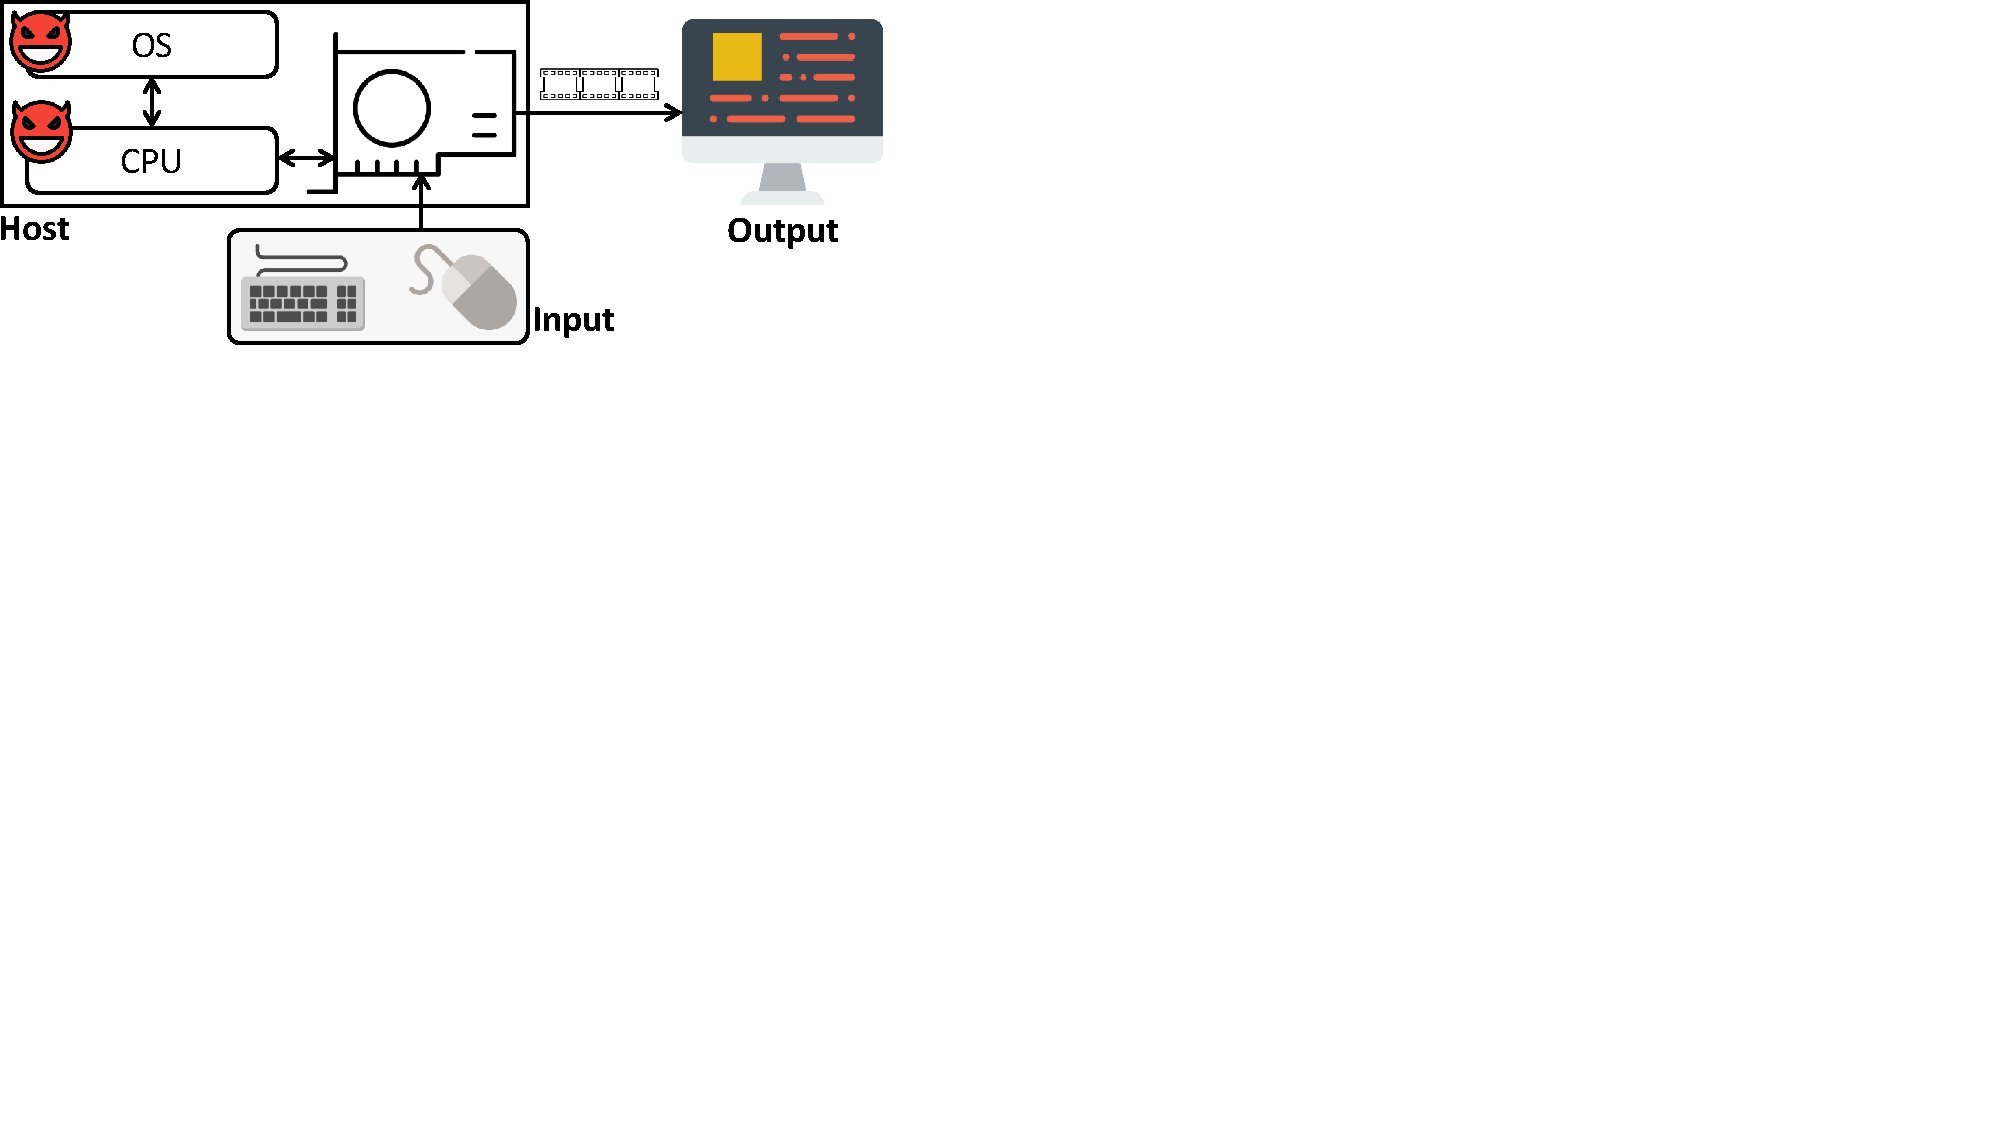
\includegraphics[trim={0 13cm 19cm 0}, clip, width=0.85\linewidth]{graphicsCard.pdf}
\caption{Integrating \name with GPUs}
\label{fig:gpuIntegration}
\centering
\end{figure}
\section{Related Work}
\label{sec:relatedWork}

In this section, we discuss some of the most relevant works to \name. We also discuss the main differences with \name to these works.


\subsection{TEE-based solutions}
There exist several solutions for integrating external devices to widely deployed TEEs: Intel SGX, and ARM TrustZone. 

\myparagraph{SGXIO} SGXIO is a proposal by Weiser et al.~\cite{weiser2017sgxio} that builds on top of Intel SGX, intending to allow SGX to interact with input-output devices. They achieve that by introducing a trusted hypervisor that allows enclaves to access virtualized peripherals. Similar to our approach, SGXIO also considers a remote adversary. However, SGXIO is rather static in nature, i.e., all the peripherals have to be set up at boot time. After the system setup phase, no changes are allowed (connect new peripherals, etc.). It is not clear how enclaves are created and get access to a peripheral while preserving the confidentiality of previous enclaves that used said peripheral. Essentially, SGXIO allows for a static extension of the hardware TCB.

\myparagraph{Graviton and systems based on it} Graviton~\cite{volos2018graviton} is a TEE that runs on an accelerator such as a graphics card. It can provide isolation between the data of multiple stakeholders that run tasks on the GPU concurrently. It also provides remote attestation of an enclave on the accelerator. Graviton was evaluated on a modern graphics card and shows that the predominant overhead stems from encryption of the communication to the processor. However, they also demonstrate that the overhead of around 20\% is tolerable. Graviton would fit very well within a \name{} as it is an excellent example of an enclave on a peripheral. It provides isolation for secret data and attestation reports. In addition, it shows that even some of the most powerful accelerators can be extended with a local TEE. Visor~\cite{visor} is a system built upon Graviton~\cite{volos2018graviton} that proposes a hybrid TEE that spans over both CPU and GPU. Visor is aimed towards privacy-preserving video analytics where the computation pipeline is shared between the CPU (non-CNN workloads) and the GPU (CNN workloads) to increase efficiency. Visor addresses micro-architectural-based side-channel attacks where a local physical attacker can use the data-dependent memory access patterns (e.g., branch-prediction, cache-timing, or controlled page fault attacks) to reveal elements on the video analysis (e.g., leaks pixel patterns). The communication between the CPU and GPU enclaves is encrypted. Additionally, Visor ensures that the traffic pattern between the CPU and GPU enclaves is independent of the video content.

\myparagraph{HETEE} HETEE~\cite{zhu2020hetee} is another proposal to extend TEEs to accelerators (specifically GPUs) without requiring changes to existing CPUs/GPUs. HETEE focuses on data center applications and proposes an extra hardware box per rack that is protected from physical attacks. This box also contains all accelerators, which it then connects to compute servers in the same rack. Each enclave then runs on a dedicated compute server and a connected accelerator. In essence, the HETEE box provides secure routing of accelerators to dedicated compute servers. In contrast to HETEE, we aim to be able to execute multiple composite enclaves on the same compute server. 


\myparagraph{ARM TrustZone and systems based on it} TrustZone is a system TEE provided by ARM for their system-on-chips (SoC)~\cite{winter2008trusted}. TrustZone applications run on top of a secure OS that is trusted and isolated from the standard operating system (also known as the rich OS). Isolation between the two worlds is achieved by an extra bit on the bus. 
%and some additional configurable components such as the TrustZone Address Space Controller (AZASC). The AZASC is a dedicated hardware component on the SoC that may permit and refuse some access to memory. 
However, there is no isolation between different TrustZone applications. Due to this limitation, mobile phone manufacturers usually only allow TrustZone applications that are signed by them. % --  a restricted version of the local attestation. 
TrustZone only provides the lower level isolation property between the rich OS and the secure OS. Everything else, i.e., isolation between TrustZone applications, remote attestation, etc., has to be added to the secure OS~\cite{ning2014samsungknox}. There have been many proposals that try to improve on the capabilities of TrustZone~\cite{brasser2019sanctuary,hua2017vtz}. Sanctuary~\cite{brasser2019sanctuary} enables user-space TrustZone enclaves. Sanctuary achieves isolation by running enclaves in their own address space in the normal world. However, Sanctuary is very similar to Intel SGX, and thus, it does not extend to peripherals.
%Similar to these proposals, TrustZone could also be extended in the direction of \name{} to support \nameenclave{}s. 
There exist proposals that enable additional security properties such as a trusted path by enabling direct pairing of peripherals (e.g., the touchscreen) to the TrustZone application. Such proposals include TruZ-Droid~\cite{TruZ-Droid}, TrustUI~\cite{trustUI}, SeCloak~\cite{SeCloak}, VButton~\cite{VButton}. All of these solutions do not provide any form of peripheral attestation similar to \name{}. They also do not consider other peripherals or how to dynamically allow an enclave to access a peripheral previously used by another enclave. Moreover, as mentioned earlier, the absence of isolation between the TrustZone applications makes the proposal mentioned above weak in inter enclave isolation guarantee.


\subsection{Other isolation methods} 

Minimal hypervisors or operating systems~\cite{herder2006minix,klein2009sel4} can also achieve isolation, and some are even formally verified~\cite{klein2009sel4}. Usually, such hypervisors do not include attestation, but the cost of adding that should be very low. A \name{} could also be based on a microkernel such as seL4. One would have to add an interface for the malicious OS running in a virtual machine to interact with enclaves that run directly on top of seL4, similar to other pure hypervisor-based isolation systems~\cite{virtualGhost,Overshadow,InkTag,TrustVisor,SplittingInterfaces,terra}. It might even be possible to formally prove such modifications to provide an even stronger assurance of isolation. Similar to other pure hypervisor-based isolation system include Virtual Ghost~\cite{virtualGhost}, Overshadow~\cite{Overshadow}, InkTag~\cite{InkTag}, TrustVisor~\cite{TrustVisor}, Splitting Interface~\cite{SplittingInterfaces}, Terra~\cite{terra} etc.  The hypervisor is also in charge of the scheduling, resulting in a significantly bigger TCB than \name. Moreover, in none of the hypervisor-based proposals, platform awareness and platform-wide attestation are considered. Isolation is the sole objective of these proposals.

\subsection{Bump in the wire-based solutions} 

Fidelius~\cite{Fidelius}, ProtectIOn (refer to Chapter~\ref{ch:protectIOn}), IntegriScreen (refer to Chapter~\ref{ch:integriscreen}), FPGA-based overlays~\cite{fpga_overlay}, IntegriKey (refer to Chapter~\ref{ch:integrikey}) are some of the trusted path solutions that use external trusted hardware devices as intermediaries between the platform and IO devices. These external devices create a trusted path between a remote user and the peripheral and enable the user to exchange sensitive data securely with the peripheral in the presence of an attacker-controlled OS. Such solutions provide a loose notion of platform awareness and are focused on IO devices. Platform-wide attestation and strong isolation guarantee are out-of-scope of such proposals. 



% \begin{table*}[t]
%   \centering
%   \resizebox{\textwidth}{!}{%
%     
\newcommand{\yes}{\CIRCLE}
\newcommand{\no}{\Circle}
\newcommand{\yesno}{\LEFTcircle}
% \newcolumntype{Y}{>{\centering\arraybackslash}X}
\begin{tabular}{@{}lcccccccccccccccc@{}}
% \begin{tabularx}{\textwidth}{@{}lcclclYYYlYYYlYYY@{}}
% \footnotesize
% \begin{tabular}{@{}lcccccccccccccccc@{}}
\toprule
    & \multicolumn{4}{c}{Platform Awareness} &  & \multicolumn{11}{c}{Isolation between Partitions} \\ \cmidrule(lr){2-5} \cmidrule(l){7-17} 
    & \multicolumn{2}{c}{Attestation} &  & \multirow[c]{2}{*}[-3pt]{\begin{tabular}[c]{@{}l@{}}Bidirectional\\ Awareness\end{tabular}} &  & \multicolumn{3}{c}{Spatial} &  & \multicolumn{3}{c}{Temporal} &  & \multicolumn{3}{c}{Fault} \\ \cmidrule(lr){2-3} \cmidrule(lr){7-9} \cmidrule(lr){11-13} \cmidrule(l){15-17} 
    & Enclave & Platform &  &  &  & \multicolumn{3}{c}{Core/SoC/Platform} &  & \multicolumn{3}{c}{Core/SoC/Platform} &  & \multicolumn{3}{c}{Core/SoC/Platform} \\ \midrule
SGX~\cite{costan2016intel} & \yes & \no &  & \no &  & \yes & \no & \no &  & \no & \no & \no &  & \yes & \yes & \no \\
Sanctum~\cite{costan2016sanctum} & \yes & \no &  & \no &  & \yes & \no & \no &  & \yes & \yes & \no &  & \yes & \yes & \no \\
Keystone~\cite{keystone} & \yes & \no &  & \no &  & \yes & \no & \no &  & \yesno & \yesno & \no &  & \yes & \yes & \no \\
Sancus~\cite{noorman2013sancus} & \yes & \no &  & \no &  & \yes & ? & \no &  & \no & \no & \no &  & \yes & ? & \no \\
TrustZone & ? & \no &  & \no &  & \yesno & \yesno & \no &  & \no & \no & \no &  & \no & \no & \no \\
Samsung Knox & \yes & \no &  & \no &  & \yesno & \yesno & \no &  & \no & \no & \no &  & \no & \no & \no \\
Sanctuary~\cite{brasser2019sanctuary} & \yes & \no &  & \no &  & \yes & \no & \no &  & \no & \no & \no &  & \yes & ? & \no \\
TPM & ? & \no &  & \no &  & \no & \no & \no &  & \no & \no & \no &  & \no & \no & \no \\
DRTM & \yes & \no &  & \no &  & \no & \no & \no &  & \no & \no & \no &  & \no & \no & \no \\
XOM~\cite{lie2000xom} & \yes & \no &  & \no &  & \no & \no & \no &  & \no & \no & \no &  & \no & \no & \no \\
Aegis~\cite{suh2003aegis} & \yes & \no &  & \no &  & \yes & \no & \no &  & ? & ? & \no &  & ? & ? & \no \\
% Bastion & \yes & \no &  & \no &  & \yes & \no & \no &  & ? & ? & \no &  & ? & ? & \no \\ \bottomrule
% \end{tabularx}
\end{tabular}
%   }
%   \caption{Comparison between traditional TEEs.\todo{Fill remaining question marks. Add daggers for all isolation facilitated by MMU}\todo{Change to the new requirements}}
%   \label{tab:comparison}
% \end{table*}


%\section{Attacks}
\label{sec:attacks}
 
Here we describe the attacks that our proposed system \toolname solves.

\subsection{Compromised host system}

Recent reports have shown that government authorities are increasingly able to compromise operating systems on both desktop and mobile platforms~\cite{}.
We therefore assume an attacker who compromises the operating system and is able to passively eavesdrop all messages displayed to the user.
These include messages the user inputs to the application. Moreover the attckacker can also compromised the hardware to get sensitive information from the peripheral devices. \usb devices assume that the \usb drivers i.e. the operating system and the host system is trusted. By using compromised operating system and the hardware the attacker can effectively plant a keylogger/screen readout which can transmit all the sensitive information the user provides/sees. Recent reports shows that there exists malwares which take screen shot of mobile devices in every fixed interval and send them to the attacker. Such can be effective against secure end-to-end encrypted messaging applications such as WhatsApp, Signal, Telegram etc.



\subsection{Phishing attacks}
\label{sec:attacks:phishing}

\subsubsection{Remote phishing attack} 
\label{sec:attacks:remotePhishing}

This is the classical phishing attack which may involve social engineering. The attacker remains remote to the target host system and serves pages that looks identical to a legitimate website. One such example can be banking or social media sites that contains lots of sensitive information. There the attacker presents a link to the victim (via messages, emails etc). In plain sight, the link looks identical to most of the people except very few changes (such as \texttt{www.facebook.com} and \texttt{www1.facebook.com}). Moreover the attacker designs the web pages in such a way that it appears identical to the legitimate website. This attack tricks the users into entering sensitive information (such as login credentials or sensitive personal information).

\subsubsection{Local phishing attack}
\label{sec:attacks:localPhising}

Local phishing attack is more sophisticated attack than the aforementioned attack (remote attack, refer Section~\ref{sec:attacks:remotePhishing}) where the attacker completely compromises the host system. The attacker can manipulate the display to show information which may appear legitimate. Such as the display drive renders \ssl\ lock logo on the browser so that the forged site appears to have an \https\ connection with the server. Apart from this the attacker can also manipulate input fields and/or modify the data in the input field. One such example is: the attacker changes the input field of an online banking site where the input field specifies how much money to send to the beneficiary. The attacker can change this value when sending it to the website. In this attack, the user can not detect such changes as the attacker does not show these changes on the display.



\iffalse
\subsection{Broad scale surveillance}

This include attackers of very high computation power and networking capability to compromise  a wide array of host systems that includes personal computers and mobile devices. Recent reports shows that there exists malwares which take screen shot of mobile devices in every fixed interval and send them to the attacker. Such can be effective against secure end-to-end encrypted messaging applications such as WhatsApp, Signal, Telegram etc. The attacker can extract all the secret communication in plain text by infecting the mobile devices/PCs or compromising the entire host system.

\myparagraph{keyloggers.} Key loggers can be both software and/or hardware backed. The hardware keylogger requires keylogger device to be installed between the peripheral device and the host system. This attack is realizable when the host system is untrusted. The software based keylogger is a n application with records and sends keyboard and mouse activities to the attacker. We can also assume a compromised operating system to execute this attack.

\subsection{Traffic analysis}

%\iffalse
\subsection{Side channel attacks on host system}
\subsubsection{Power analysis}
\subsubsection{Timing leakage}
\subsubsection{USB device cross-talk}
\fi

\section{Conclusion} 
\label{integriscreen:sec:conclusion}

In this chapter, we explore the idea of \emph{visually supervising} user's IO data to provide IO integrity against a compromised host. We use a smartphone to capture the client's screen and enforce the integrity of the web rendered on the screen, alongside the input data the user submits on the web form. We show the feasibility of this approach by developing a fully functional prototype on an Android smartphone, evaluating it with a series of experimental tests, and running a user study to measure participants' responses to simulated attacks.
Considering the rapid increase in processing power and camera quality of smartphones, but also novel platforms such as augmented reality headsets and smart home assistants, we envision such systems that supervise user's IO will be ubiquitous.

\section*{Acknowledgments}
The authors would like to thank the anonymous reviewers and our shepherd Kevin Butler. This research has been partially supported by the Zurich Information Security and Privacy Center (ZISC).


\bibliographystyle{IEEEtran}


\bibliography{references}

\appendix
\subsection{Proof for IO Integrity}
\label{appendix:security}

In this appendix, we provide a formal proof of the following property: \emph{without protecting both input and output integrity, none of them can be achieved}. 


%\subsection{Interaction Protocol} 
%\label{appendix:security:protocol}

\myparagraph{Interaction protocol}
To simplify the proof, we model the interaction between the user, the host, and the remote server as a finite state automaton (FSA).
The interactions between the server (\server), the user (\user) and host (\host) are depicted in the FSA in Figure~\ref{fig:fsm}.

\begin{figure}[h!]
\begin{center}
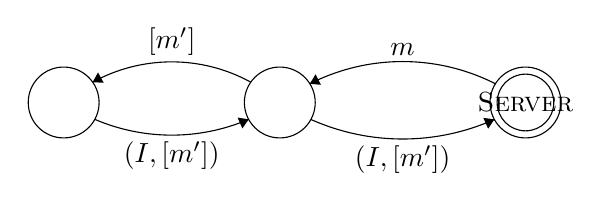
\begin{tikzpicture}[scale=0.15]
\tikzstyle{every node}+=[inner sep=0pt]
\draw [black] (66,-23.1) circle (3);
\draw (66,-23.1) node {\server};
\draw [black] (66,-23.1) circle (2.4);
\draw [black] (45.2,-23.1) circle (3);
\draw (45.2,-23.1) node {\host};
\draw [black] (26.9,-23.1) circle (3);
\draw (26.9,-23.1) node {\user};
\draw [black] (47.743,-21.516) arc (116.95563:63.04437:17.332);
\fill [black] (47.74,-21.52) -- (48.68,-21.6) -- (48.23,-20.71);
\draw (55.6,-19.13) node [above] {$m$};
\draw [black] (29.352,-21.382) arc (118.8302:61.1698:13.89);
\fill [black] (29.35,-21.38) -- (30.29,-21.43) -- (29.81,-20.56);
\draw (36.05,-19.16) node [above] {$[m']$};
\draw [black] (42.565,-24.526) arc (-66.78269:-113.21731:16.527);
\fill [black] (42.57,-24.53) -- (41.63,-24.38) -- (42.03,-25.3);
\draw (36.05,-26.36) node [below] {$(I,[m'])$};
\draw [black] (63.369,-24.535) arc (-65.91058:-114.08942:19.034);
\fill [black] (63.37,-24.53) -- (62.43,-24.4) -- (62.84,-25.32);
\draw (55.6,-26.69) node [below] {$(I,[m'])$};
\end{tikzpicture}
\end{center}
\caption{Finite state machine that depicts the interaction between the user (\user), host (\host) and the server (\server).}
\label{fig:fsm}
\end{figure}

\server sends a message $m$ to \host. One can assume $m$ to be the HTML, JavaScript, and other data send from \server as a HTTP response. We denote $[m]$ to be the render of $m$ by the \host. As \host is malicious, it can transform $m$ to $m'$. Note that the transformation is public knowledge and is deterministic. If $m\neq m'$ then given $[m]$ and $[m']$, \server can determine that $[m]\neq [m']$. We denote the user input to be $I$, which corresponds to a specific $[m]$. 
%Note that the communication channel between \server to \user is neither authenticated, neither confidential. But the communication channel from \user and \server is authenticated. 
In this model, we simplify the user input by assuming that the \user only provides an input $I$ only after observing a message transformation $[m]$. The user provides both her input $I$ and transformation $[m']$ observed by her to \host. The interaction loop between \host and \user can continue until \user finishes her input. After every input \host hands over new message transformation to \user (either result of the input or new message from \server or both). Once the user provides all her inputs, \host send the pairs $(I, [m'])$ to \server.

We also define two mappings:
\begin{align*}
\texttt{Input()}&:[m]\rightarrow I \\
\texttt{Transform()}&:m,I\rightarrow [m'],\ \exists i\in I:i=\phi
\end{align*}
Both of them are \emph{bijective}.

One trace of the protocol transcript is depicted in Figure~\ref{fig:protocol}. As described in the FSM, \server receives traces of message transformation ($[m']_1,[m']_2,\ldots,[m']_n$) and corresponding inputs ($I_1,I_2,\ldots,I_n$). From these traces \server could determine of all the $[m']_i$ are in proper form by verifying if $[m]_i=[m']_i$.

\begin{figure}[t]
\begin{center}
\tikzset{
  every picture/.append style={
    transform shape,
    scale=0.8
  }
 }
\begin{sequencediagram}
\newinst{u}{\user}
\newinst[3]{h}{\host}
\newinst[3]{s}{\server}
\mess{s}{$m$}{h}
\mess{h}{$[m']_1$}{u}
\mess{u}{$I_1,[m']_1$}{h}
%\mess{h}{$[m']_2$}{u}
%\mess{u}{$I_2,[m']_2$}{h}
\mess{h}{...}{u}
\mess{u}{...}{h}
\mess{h}{$[m']_n$}{u}
\mess{u}{$I_n,[m']_n$}{h}
\mess{h}{$I_1,I_2,...,I_n$}{s}
\mess{h}{$[m']_1,[m']_2,...,[m']_n$}{s}
\end{sequencediagram}
\end{center}
\caption{Protocol transcript between the \server, \user and \host that shows one trace from the FSM depicted in Figure~\ref{fig:fsm}.}
\label{fig:protocol}
\end{figure}


\begin{definition}{\textbf{Input integrity}}
\label{def:inputIntegrity}
Assume that \server handed a message $m$ to \host where the proper message transformation is $[m]$. The host changes the message transformation to $[m']$ where $[m']\neq [m]$. We also define correct \user input to be $I$ when \host sends a correct message transformation $[m]$ to \user. We define input integrity as the property where the \server does not accept input $I'$ where $I'\neq I$from \user if the \host changes the message transformation.
\end{definition}

\begin{definition}{\textbf{Output integrity}}
\label{def:outputIntegrity}
Assume that \server handed a message $m$ to \host where the proper message transformation is $[m]$. Output integrity defines that in all circumstances, \user receives the correct message transformation $[m]$ from \host.
\end{definition}

\myparagraph{Verification process} \server checks $\forall i=1\ldots n$ $$[m']_i = \texttt{Transform}(m_{i-1}, I_{i-1})$$ where $I_0=\phi$.

\begin{theorem}
\label{theorem:th1}
If \user does not send all the transformations till $[m']_i$ corresponding to the input $I_i$, input integrity can not be achieved. 
\end{theorem}

\begin{IEEEproof}
If \user does not attach all the transformation till $[m']_i$, i.e., $[m']_1, [m']_2, \ldots, [m']_{i-1}, [m']_i$  corresponding to inputs $I_1, I_2,\ldots, I_{i-1}, I_i$, then the server can not verify all the transformations corresponding to the input. \host could modify a specific $[m]_x$ to influence \user input.
\end{IEEEproof}

\begin{theorem}
\label{theorem:th2}
If the channel from \user and \server is not authenticated, input integrity is not achievable. But the channel from \server to \user does not require to be secure as long a \user provides the message transformation $[m']_i$ corresponding to every input $I_i$.
\end{theorem}

\begin{IEEEproof}
The proof is trivial. If the channel from \user to \server is not authenticated, any input provided by \user can be manipulated by \host without a trace. Hence input integrity is not achievable. As long as \user sends message transformation along with the input, a manipulated message transformation bt \host would be detectable by \server (see Theorem~\ref{theorem:th1}).
\end{IEEEproof}

\begin{theorem}
\label{theorem:th3}
Ensuring output integrity also ensures input integrity provided there is an authenticated channel from \user to \server.
\end{theorem}

\begin{IEEEproof}
This proof is also trivial. As we describe in the Definition~\ref{def:inputIntegrity} and~\ref{def:outputIntegrity}, if all the message transform from \host $[m']=[m]$, and \host always executes \texttt{transform()} properly, the input integrity is preserved. As \name ensures output integrity and all the input from the user is signed by the \device, \name preserves input integrity. 
\end{IEEEproof}


%\section*{Implementation Details}
%\label{appendix:implementation}

\subsection{Implementation of \name Components}
\label{appendix:implementation}


In the following, we provide the implementation details of the \name components presented in the previous sections. 

\myparagraph{QR code generation \& UI specification}
\label{sec:prototype:impl:qr}
%
QR code generation phase is executed by \name JS that transforms the UI elements of a sensitive web form to a UI specification encoded in a QR code (we use QRCode.js, a \js library to produce QR codes). Section~\ref{sec:systemDesign:transformation} provides the high-level concept of generating the QR code from the webpage UI elements. UI elements that require IO integrity protection can be marked by the developers in the \html source. As illustrated in Figure~\ref{fig:transformation}, the \html UI elements: `\texttt{Sensitive field 1}' and `\texttt{Sensitive field 2}' have the additional attribute \texttt{protect=``true''}. %(one concrete example is illustrated in Figure~\ref{fig:transformation}). 

The \name JS iterates through the HTML elements that have the \texttt{protect} attribute enabled and extracts the information such as the name of the label or the type of the UI element. \device uses preloaded size parameters to specify the size of a text field, button, etc. in case the size is not explicitly mentioned in the HTML source. One important attribute for a UI element in the specification is the \texttt{trigger}. For example, in Specification~\ref{snippet:UISpecification}, the \texttt{OK} and the \texttt{cancel} buttons have an attribute \texttt{trigger}. This attribute is Boolean can be either \texttt{true} (corresponding to \texttt{OK}) or \texttt{false} (corresponding to \texttt{Cancel}) value. The value \texttt{true} denotes that the \texttt{OK} button can submit the values that are provided by the user. The \texttt{false} attribute denotes that hitting the \texttt{cancel} button abort the form altogether. 

The QR code generation phase is between \one and \two in Figure~\ref{fig:transformation} where the \name JavaScript snippet transforms the UI elements to a UI specification language in a QR code that can be interpreted by the \device. The UI specification corresponding to the \html source (in Figure~\ref{fig:transformation}) is provided in Specification~\ref{snippet:UISpecification}. Note that the specification is highly flexible, allowing adjustable size for the form, individual UI elements, gaps between them, etc. This allows the \device to faithfully recreate the UI that is very close to the actual form UI that the served by the web severer. 
%Such allows negligible user habituation. 

\myparagraph{Bitmap generation}
\label{sec:prototype:impl:bitmap}
%
The \device reads the QR code from the HDMI frame and generate the UI overlay bitmap from it. We have used the \texttt{piCamera} library to intercept the HDMI frames and generate the UI on top of it. Our \name prototype implements the most frequently used HTML input elements~\cite{html_elements} that are common in sensitive forms. 

\myparagraph{Detection of mouse pointer}
\label{sec:prototype:impl:mouse}
%
Initially, when the system boots up the \device perform the calibration phase (see Section \ref{sec:systemDesign:analysis:calibration}) to synchronize its coordinates of the pointer with the host. The detection of the mouse pointer is implanted partially on the raspberry pi 4 (\six in Figure~\ref{fig:prototypeAll}), while the mouse intercepting is done in the Arduino Due (\three in Figure~\ref{fig:prototypeAll}). The Due gathers the raw mouse data (in terms of displacement measurements $(\Delta x_i, \Delta y_i)$) and sends them to the Pi over \texttt{Serial} interface.  To guarantee that the \device and the host interpret displacement events likewise, the Pi performs an adjustment operation. This operation consists of the \device detecting the exact position of the host pointer in the HDMI frame by analyzing a small square of the frame (200 x 200 px) around its pointer coordinates. Considering that the \device gets raw HDMI frames and pointer images are static, we use the lightweight \texttt{template matching} algorithm of the OpenCV library for the detection.

\myparagraph{Implementation of the upstream channel}
\label{sec:prototype:impl:upstream}
%
The \emph{upstream} channel, i.e., the data from the \device to the remote server is transmitted using the \name JavaScript snippet that is served by the remote web server. The \name JavaScript snippet uses a hidden text field to accept data coming from the \device. The \device emulates itself as a composite human interface device (HID) when it is connected to the host. The \device emulates keystrokes that transmit encoded data (base64) to the \name JavaScript snippet that is sent to the remote server via \texttt{XMLHttpRequest} call.

\begin{figure}[t]
\centering
\includegraphics[trim={0 10cm 17cm 0}, clip, width=0.85\linewidth]{keyExchange_1.pdf}
\caption{\textbf{Establishing \tls.} A snapshot of the key exchange web page that is used to communicate the public certificates of the device and the remote server.}
%\spacesave
\label{fig:keyExchange}
\centering
\end{figure} 

\myparagraph{Establishing \tls}
\label{sec:prototype:impl:tls}
%
For the IO confidentiality, the \device and server create a \tls channel. When the user opens up a secure webpage, key exchange is the first step that takes place. We assume that the remote server already has the \device's certificate, or some offline registration takes place. An instance of the key exchange protocol of \name is illustrated in Figure~\ref{fig:keyExchange}. The flow of the key exchange mechanism is as the following:
%\vspace{-10pt}
\begin{mylist}
  \item[\one] The server delivers a web page with a QR code that encodes the signed public key of the server (server hello in TLS). 
  \item[\two] The device captures every frame until it detects a QR code. Then, it decodes the QR code and verifies the public key and derives the shared secret using Diffie-Hellman protocol~\cite{blake1998authenticated}. 
  \item[\three] The device then sends its signed public certificate to the host, which forwards it to the server.
  \item[\four] The remote server gets the signed certificate from the \device, verifies it, and finally derives the shared secret.
\end{mylist}

\begin{figure}[t]
\centering
\includegraphics[trim={0 12cm 10cm 0}, clip, width=\linewidth]{cursorDetect.pdf}
\caption{\textbf{Cursor detection on the HDMI frame.} The figure shows \name mouse pointer tracking. \one shows the captured HDMI frame captured by B101 HDMI to CSI bridge. \two shows the cropped HDMI frame based on the mouse position received by the \device. \three shows the detected mouse pointer. For testing, we program the \device to put a rectangle around the pointer. \four shows one of the pointer templates that we used in our OpenCV routine.}
%\spacesave
\label{fig:cursorDetect}
\centering
\end{figure} 


\myparagraph{HID Drivers}
We use Arduino prototype development board as the HID drivers. Figure~\ref{fig:prototype} shows an Arduino Due, and a Zero board where the Due connects to the HIDs via the native USB port and the Zero relays the HID data to the Raspberry Pi (RPi). The Due and the Zero boards are connected over $I^2C$ interface. As both Due and Zero only have one native USB port on each of them, we were forced to use two boards as an HID interceptor and relay. The Zero relays the HID signals both to the connected host (over native USB) and to the RPi (over serial interface). The connection from the Zero to the host is one way and emulates a composite HID. While the connection between the Zero and the RPi is bidirectional. The HID drivers are implemented using the native Arduino \texttt{keyboard} and \texttt{mouse} library. On the RPi, no HID drivers were needed as the RPi receives processed HID data from the Zero (for the pointer: displacement over x and y-axis and for keyboard, ASCII characters).


\myparagraph{HDMI Interceptor, Relay and Overlay}
The RPi along with the Auvidea B101 HDMI to CSI bridge, acts as the HDMI interceptor and relay. The B101 board converts HDMI signals from the host as a camera input (via the CSI interface) to the RPi. This allows the RPi to access the HDMI frames as a stream of JPEG frames. The HDMI out of the RPi acts as the relay that connects to the monitor. On the RPi, we use Picamera API~\cite{picamera} to access the HDMI frames. The B101 is capable of processing 25 frames at 1080p resolution. Hence, this is the hardware bottleneck of our implementation. However, the upcoming B112 board
%\footnote{still in development: \url{https://auvidea.eu/showcase/}.} 
could solve this performance issue.

On the RPi, the overlay and HDMI out is implemented using Java SWT. Using SWT, we create a full-screen window that is shown on the monitor. The SWT class polls the HDMI frames and process them as individual JPEG images via the \texttt{BufferedImage} class. This allows the overlays to be drawn on the HDMI images efficiently. The Java program uses a QR code interpreter to extract the UI specification. Based on the UI specification, it creates the geometrical shapes (corresponding to the UI elements) and draw them on the frames. In the current implementation of the \name, the UI elements such as button, text-field, radio button etc. are preloaded in the \device memory. Note that the current implementation of \device is based on the RPi. But one could implement such functionality on an FPGA, reducing the TCB even more. 


\myparagraph{Mouse Pointer Tracking}
The pointer tracing is also executed in the aforementioned Java program using simple object detection technique suppled by the OpenCV API. Figure~\ref{fig:cursorDetect} shows one screenshot of the pointer detection. The Figure shows the entire HDMI frame, the cropped frame of resolution $200 \times 200$ px (based on the mouse input data), the detected pointer in the cropped frame and the cursor template that is used by the object detection algorithm.





\end{document}


%%Abstract submission

% Security and safety-critical remote applications such as e-voting, online banking, industrial control systems and medical devices rely upon user interaction that is typically performed through web applications. Trusted path to such remote systems is critical in the presence of an attacker that controls the computer that the user operates. Such an attacker can observe and modify any IO data without being detected by the user or the server. We investigate the security of previous research proposals and observe several drawbacks that make them vulnerable to attacks. Based on these observations we identify novel requirements for secure IO operation in the presence of a compromised host.
%   
% As a solution, we propose ProtectIOn, a system that ensures IO integrity using a trusted low-TCB device that sits between the attacker-controlled host and the IO devices. ProtectIOn intercepts the display signal and user inputs from the keyboard and mouse, and overlays secure UI on top of the HDMI frames generated by the untrusted host. The guiding design principles of ProtectIOn are that (i) integrity of user input and output cannot be considered separately, (ii) all user input modalities need to be protected simultaneously, and (iii) integrity protection should not rely on error prone user tasks like checking the presence of security indicators. By following these guidelines, ProtectIOn achieves strong protection for IO integrity. We also propose an extension of ProtectIOn for IO confidentiality and implement a plug-and-play prototype and evaluate its performance. 